\chapter{Ripple Phase}\label{chap:ripple}
When the temperature is reduced from the fluid phase, 
the ripple phase is observed in bilayers consisting of DMPC and DPPC lipids.
This chapter discusses X-ray scattering experiments on the ripple phase 
formed by dimyristolphosphatydylcholine (DMPC) bilayers. 

%%%%%%%%%%%%%%%%%%%%%%%%%%%%%%%%%%%%%%%%%%%%%%%%%%%%%%%%%%%%%%%%%%%%%%%%%%%%%%%
\section{Introduction}\label{sec:ripple_introduction}
The ripple phase has been a fascinating thermodynamic phase to many physicists 
and physical chemists since its discovery. It was originally observed in 
calorimetry study for alcanes by sturevant. Although this phase has never been reported to 
occur in a biologically relevant situation, it provides an interesting opportunity
to study fundamental lipid interactions and their influence on the bilayer 
shape. 

\subsection{Some history}
In the first structural study of this phase by Tardieu \textit{et al.},
the X-ray diffraction pattern from DLPC was phased by a pattern recognition
technique and the electron density map was calculated. It was shown that the structure
corresponds to a 2D oblique unit cell shown in Fig.~\ref{fig:unit_cell}.
The calculated 
electron density map showed that DLPC bilayers are height modulated
and have a smooth, asymmetric shape. 
The ripple wavelength $\lambda_r$ was reported to be 85.3 \AA, 
the lamellar periodicity $D$ 55.3 \AA, and the oblique angle
$\gamma$ 110\textdegree. 
The electron density map reported the ripple amplitude $A$ = 15 \AA\ in DLPC.

Various experiments have indicated the existence of two types of ripple phases:
the stable asymmetric and the metastable symmetric phase. In the asymmetric
phase, a plane of reflection perpendicular to the ripple wave vector is 
absent. The metastable symmetric phase has been seen in DPPC bilayers, but not
in DMPC.

\begin{figure}[htbp]
  \centering
  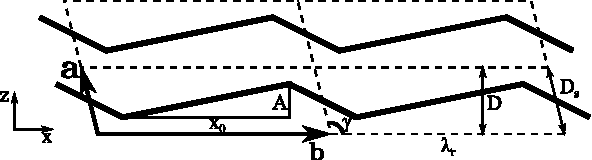
\includegraphics[width=0.8\textwidth]{figures/ripple/unit_cell}
  \caption{Lattice structure of the asymmetric ripple phase. Unit cells are shown in
  dash lines. Center of bilayers are shown by thick, solid lines. Notations 
  in the figure are ($\mathbf{a}$ and $\mathbf{b}$: lattice unit vectors),
  ($D$: $D$-spacing along $z$), ($\lambda_r=|\mathbf{b}|$: ripple wavelength), 
  ($\gamma$: oblique tilt angle), ($A$: ripple amplitude),
  ($\psi$: chain tilt angle with respect to the $z$ direction),
  and ($x_\textrm{M}$: projected length of the major arm).}
  \label{fig:unit_cell}
\end{figure}

The equilibrium structure of the ripple phase has been extensively studied by
X-ray diffraction \cite{ref:Janiak76,ref:Janiak79,ref:Tardieu73,ref:Wack89,ref:Yao91,ref:Sun96,ref:Cunningham98},
neutron diffraction \cite{ref:Mortensen88,ref:Bradshaw89}, 
AFM \cite{}, freeze fracture electron microscopy \cite{ref:Woodward96},
and freeze fracture scanning tunneling microscopy \cite{} techniques.
In the scanning tunneling microscopy experiment \cite{ref:Zasadzinski88}, 
the three-dimensional contours of the ripple phase $P_{\beta'}$ of
dimyristoylphophatidylcholine (DMPC) were imaged, and
a ripple wavelength of 130 \AA\ and an amplitude of 45 \AA\ were reported.

While many studies used multilamellar samples, the ripple phase was also found in
unilamellar vesicles, where a vesicle has only one bilayer 
\cite{ref:Mason99}.

The ripple phase has been detected in
phosphatidylcholines (PC) and phosphatidylglycerol (PG),
but no ripple phase has been observed in bilayers composed of PE headgroups.
These studies suggest that the size of headgroup has something to do with
the ripple formation. Indeed, it has been suggested that the size mismatch
between the bulky PC headgroup and hydrocarbon chains lead to tilt of 
the chains. 

From X-ray data of the DMPC ripple of unoriented samples, 
Wack and Webb \cite{ref:Wack89} argued that the ripples have a sawtooth shape,
but were unable to phase the observed pattern.
Their X-ray form factor data were later
phased by employing a modeling and fitting technique by Sun \textit{et al.}
\cite{ref:Sun96}, and the electron density map was calculated, which indicated that  
the ripples indeed have a sawtooth shape. The map also showed that
the major arm is about twice as long as the minor arm. The bilayer
thickness was found to be larger than that of the minor arm. The
value of the bilayer thickness in the major arm was comparable to the
thickness of DMPC bilayers in the gel phase.

A structural investigation by X-ray diffraction of the ripple phase of
oriented dipalmitoylphosphatidylcholine (DPPC) samples indicated that
hydrocarbon chains are packed in a hexagonal lattice with chains
tilted in the plane perpendicular to the ripple wave vector \cite{ref:Hentschel91}.
In that study, the oblique angle $\gamma$ was found to be 90\textdegree.
It is believed that the resolved structure was for the symmetric ripple,
which has been shown to be thermodynamically metastable and whose occurrence
depends on the sample history \cite{ref:Katsaras00}. 
In \cite{ref:Hentschel91}, only symmetric ripple was observed in the low angle
X-ray scattering, which seems to contradict with the metastability of this 
symmetric ripple.

Sengupta et al. \cite{ref:Sengupta03} has investigated temperature dependence of the average structure
of DMPC and concluded that there is no obvious change in the structure
as a function of temperature. On the other hand, the ripple phase composed of 
POPC showed some variation in the average structure.
Based on calculated electron density profiles and model parameters, they
argued that chains in both major and minor arms are tilted with respect to 
the stacking $z$ direction by the same amount and that 
chains are parallel to the local normal in the major arm. This argument 
was inconsistent with the findings in \cite{ref:Sun96} that
the thickness of major arm is almost identical to that of the gel phase where chains 
are tilted by $\sim$30\textdegree. To circumvent this discrepancy, 
Sengputa \textit{et al.} speculated that chains might be titled by some amount into the 
direction perpendicular to the ripple direction. This type of information
, however, is not well captured in low angle scattering data, and
wide angle scattering is essential.

In a giant unilamellar vesicle composed of a mixture of DPPC and DOPC, 
coexisting domains of L$_\beta'$ and P$_\beta'$ have been found \cite{ref:Li06}.
The P$_\beta'$ domain had lower concentration of DPPC than the L$_\beta'$
domain. Addition of anionic lipids (DOPG?) turned the gel phase domain
into the ripple phase domains. The authors concluded that reduction of 
surface tension drove highly stressed gel phase to less stressed ripple phase.

\textcolor{red}{AFM}
The ripple phase has also been observed in the top layer of 
solid supported double layers through atomic force microscopy (AFM).
The effect of the bottom layer on the top layer in the ripple phase has not been
thoroughly studied. 
It is not clear whether the structure of these ripple formation top layers
is the same as that in a bulk sample such as MLVs and oriented samples.

A few MD (molecular dynamics) simulations have shed light on molecular 
organization in the ripple phase as well. 
de Vrie \textit{et al.} \cite{ref:deVries05}
carried out atomistic simulations resulting in an
assymetric ripple where chains are gel-like in the major arm and
interdigitated in the minor side. Coarse-grain
simulations performed later essentially found the same results
\cite{ref:Lenz07}.

A theory developed by Chen \textit{et al.} \cite{ref:Chen95} has been 
successful in describing some features in the ripple phase. In this theory,
the divergence of the tilt field of lipids are coupled to the curvature 
of the bilayer. Increase in the divergence of the lipid tilt is compensated 
by increase in the curvature, leading to the observed height modulated
ripple phase. This theory predicted ripple phases with different symmetry
for chiral and achiral lipids. Later, Katsaras and Raghunathan 
\cite{ref:Katsaras95} carried out low angle X-ray scattering experiment
on regular DMPC and achiral DMPC and found that there was no structural
difference between them. 

Raghunathan theory (2011)

Schmidt theory (2013)

\begin{table}[htbp]
\centering
  \begin{tabular}{ccc}
    \hline
    $D$ & $\lambda_r$ & $\gamma$ \\
    (\AA) & (\AA) & (deg) \\
    \hline
    55.0 & 159.4 & 99.0 \\
    57.0 & 140.8 & 97.6 \\
    57.3 & 151.6 & 97.8 \\
    57.4 & 148.4 & 97.6 \\
    57.5	 & 144.1 & 97.8 \\
    57.5 & 141.9 & 98.0 \\
    58.0 & 140.1 & 98.2 \\
    \textcolor{blue}{57.8} & \textcolor{blue}{145.0} & \textcolor{blue}{98.2} \\
    58.0 & 141.7 & 98.4 \\
    59.8 & 129.6 & 97.3 \\
    60.6 & 130.1 & 97.0 \\
    61.5 & 130.8 & 96.5 \\
    62.4 & 122.0 & 95.9 \\
    63.9 & 123.1 & 94.9 \\
    64.9 & 120.3 & 92.3 \\    
    \hline 
  \end{tabular}
  \caption{Lattice constants for DMPC at $T$ = 18.0 \textcelsius\
  reported by Wack and Webb \cite{ref:Wack89} except the one colored in blue. 
  The data collected and analyzed in this thesis
  are colored blue.} 
\end{table}

\subsection{Purpose of this study}
The intial purpose of this study was limited to obtaining better data relevant
to the packing of the lipids within the sawtooth, asymmetric ripple profile 
that has been well documented \cite{ref:Sun96}. A favorite hypothesis  ... 
Structure at small length scales requires WAXS, and not just unoriented data, 
but data from oriented samples.  Previously published data suffers from loss 
of in-plane scattering intensity that we are able to obtain by using a wide 
angle scattering method, called  transmission WAXS (tWAXS), where the x-rays 
go through the substrate before scattering from the sample.  As it was 
necessary to confirm the usual low angle structural parameters for our 
samples, we also obtained LAXS data.  Remarkably, we observed many more well 
separated reflections than in the Wack and Webb data  from unoriented samples 
that were used to obtain the best electron density profile \cite{ref:Sun96}.  
These remarkable data are shown in Fig.\ref{fig:ripple_laxs_images}.  
This meant that an additional project became obtaining a high resolution EDP 
to improve upon the previous low resolution EDP.

The extraction of bilayer form factors required to obtain electron density 
profiles is rather more demanding for oriented samples than for unoriented 
samples; this is documented in Sections 3.3-3.5 after describing the samples 
and the X-ray set-up in Section 3.2.  Obtaining the phases is also more 
challenging as described in Section 3.6 before giving final results in 
Section 3.7.  These structural results are required for the interpretation 
of the wide angle data, both near grazing incidence nGWAX and transmission 
tWAXS.  

\begin{figure}[htbp]
  \centering
  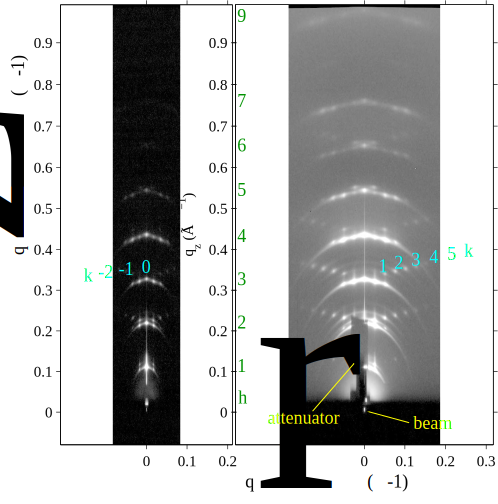
\includegraphics[width=0.95\textwidth]{figures/ripple/ripple083and085}
  %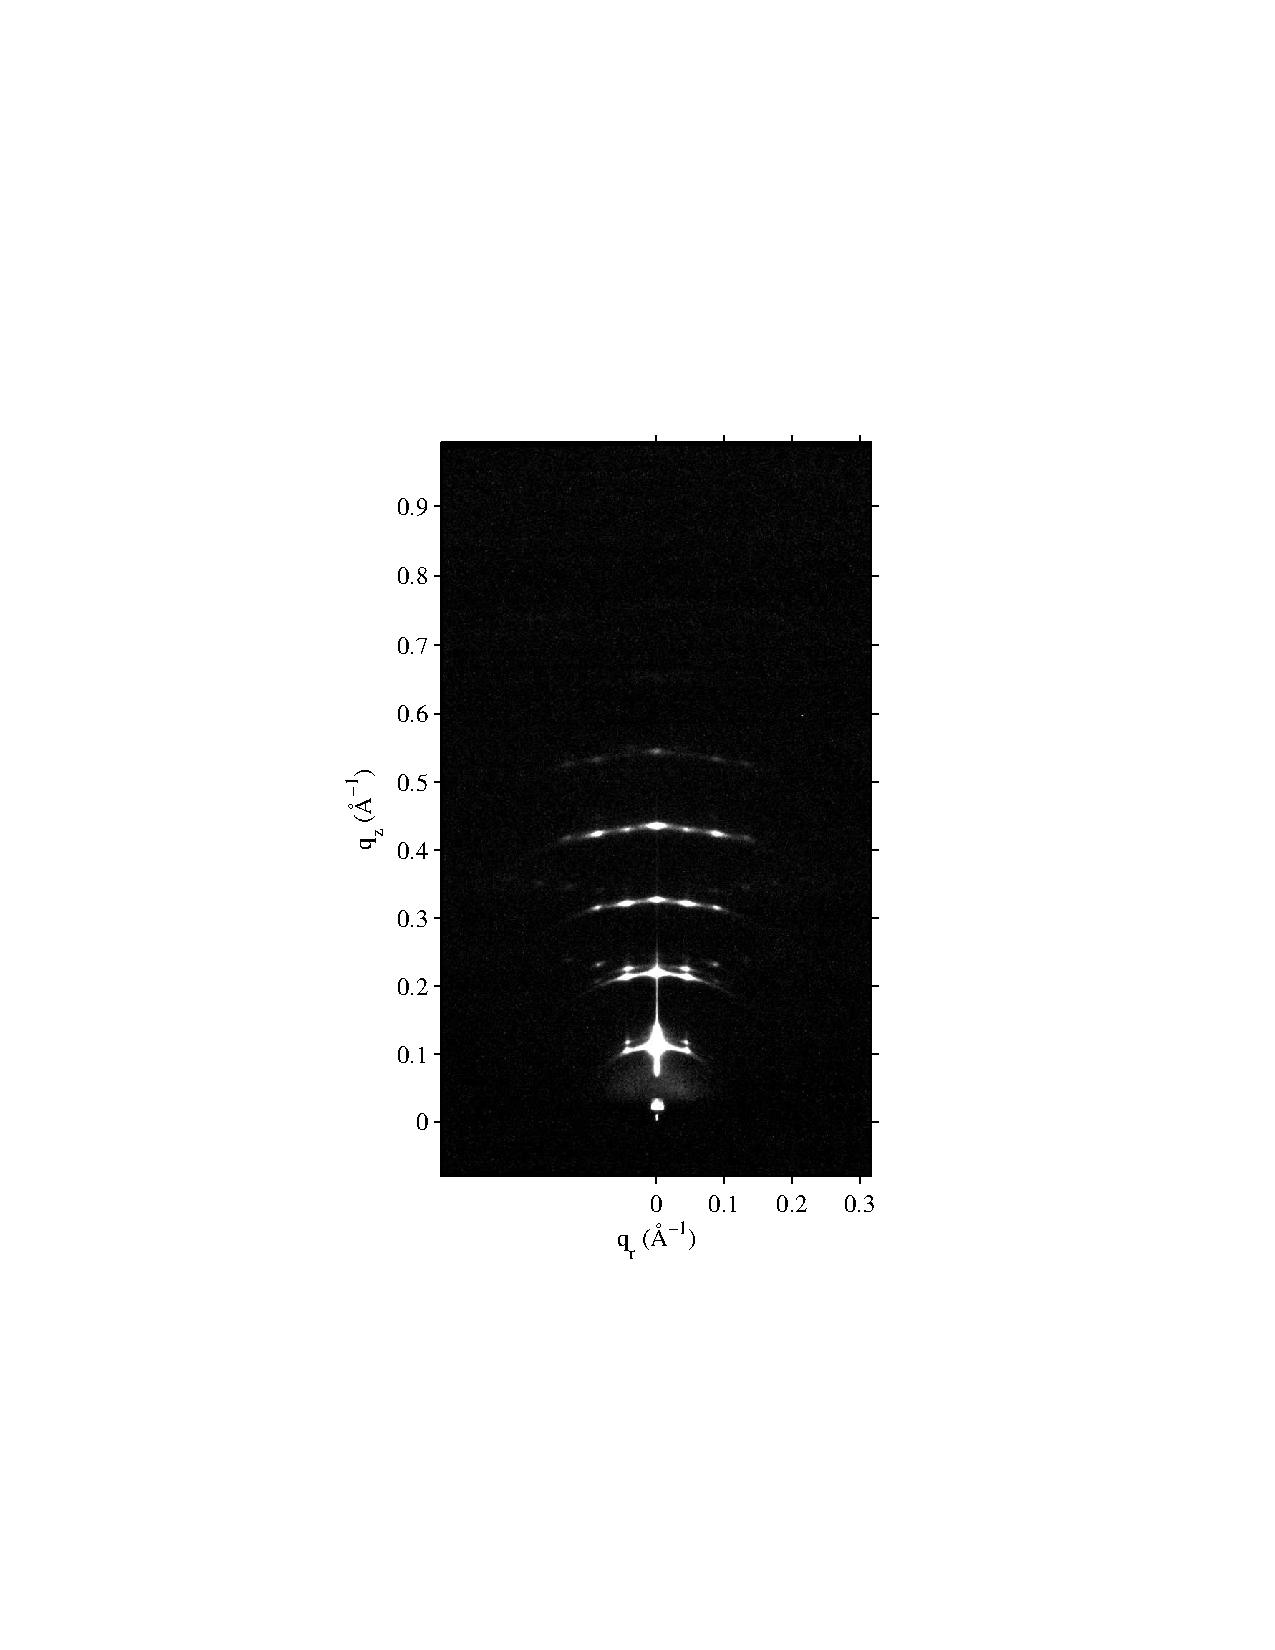
\includegraphics[trim=160 180 160 180,clip,width=0.49\textwidth]{figures/ripple/ripple083}
  %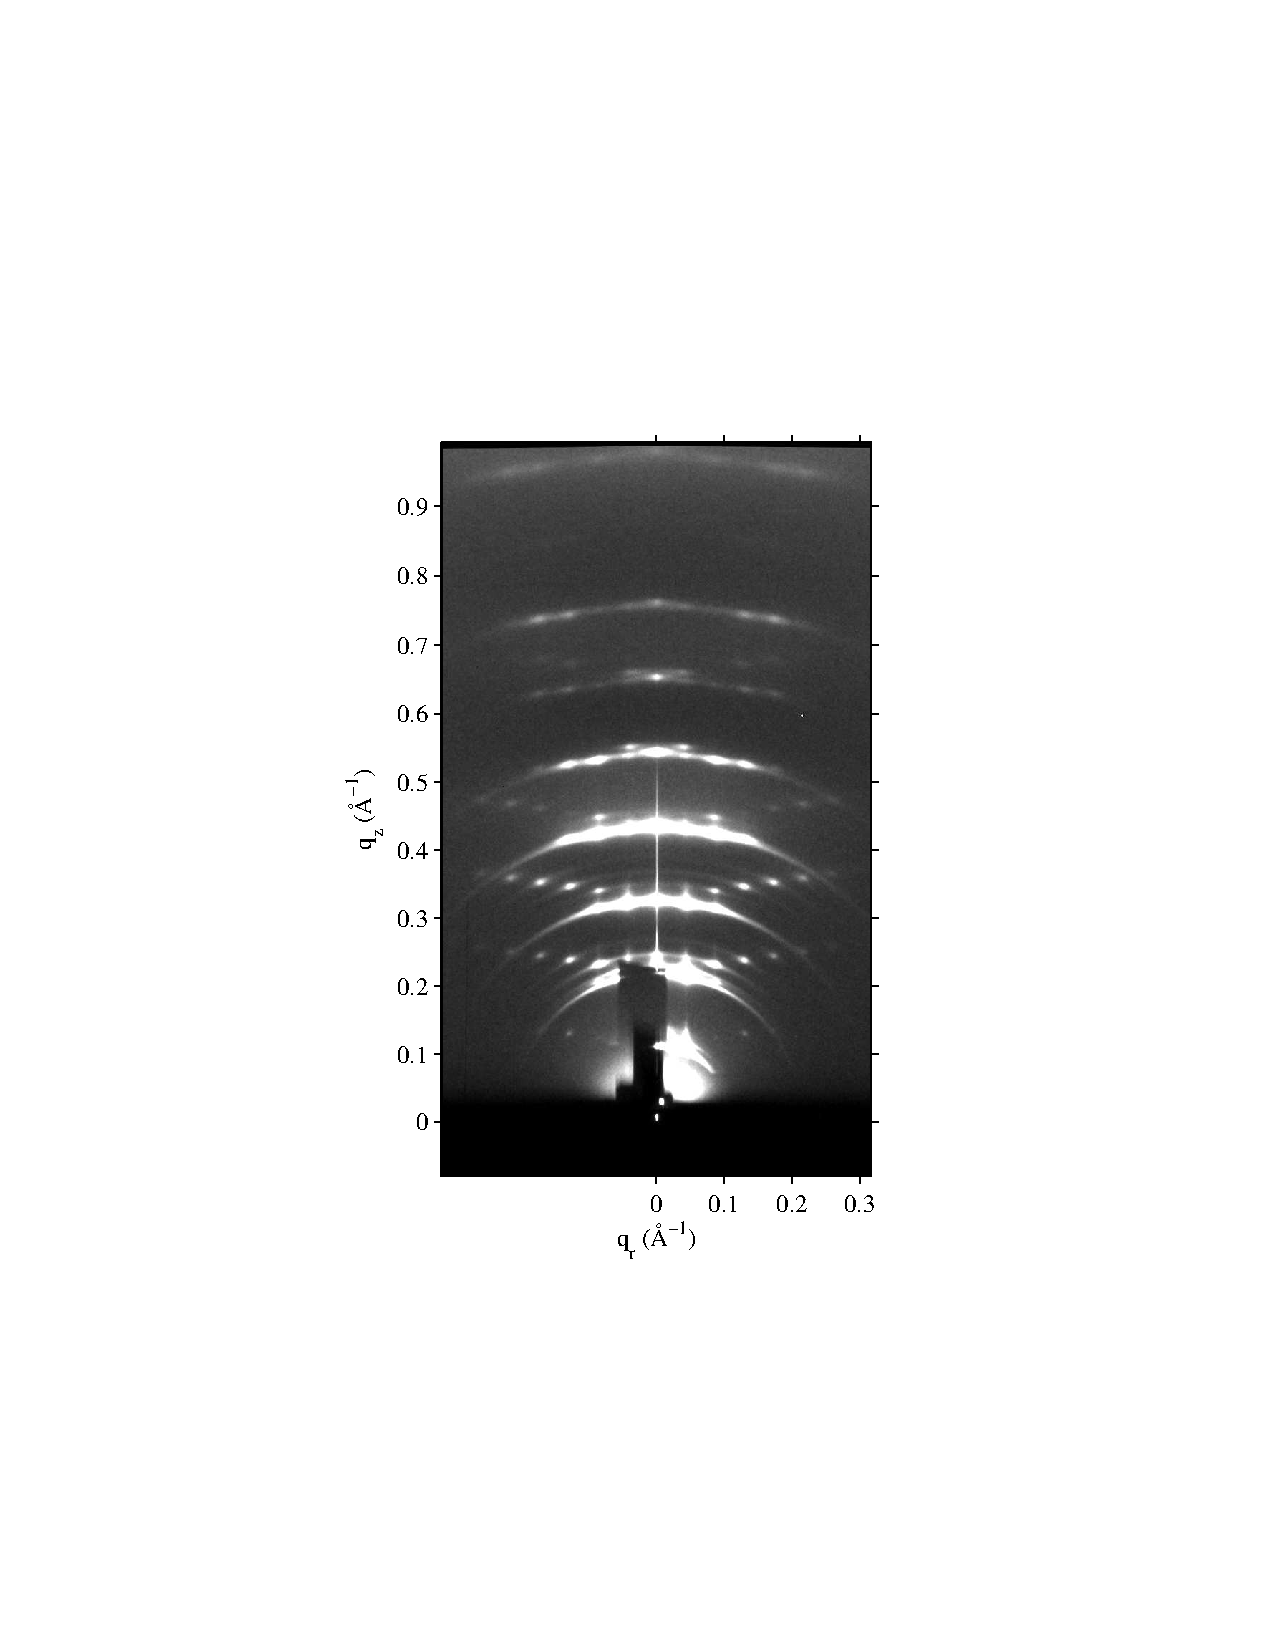
\includegraphics[trim=160 180 160 180,clip,width=0.49\textwidth]{figures/ripple/ripple085}
  \caption{1 second exposure (left) and 60 second exposure (right) of the low
  angle X-ray scattering from the DMPC ripple phase in gray log scales. 
  The index $h$ is 
  labeled in green. $(3,k)$ reflections are identified in cyan. 
  The shadow cast by 100 $\mu$m thick molybdenum attenuator blocking
  strong (1,0) and (2,0) orders in the right image is labeled as attenuator
  and extends from $q_z$ = 0 \AA$^{-1}$ to 0.2 \AA$^{-1}$.
  $D$ = 57.8 \AA, $\lambda_r$ = 145.0 \AA, and $\gamma$ = 98.2\textdegree.}
  \label{fig:ripple_laxs_images}  
\end{figure} 

%%%%%%%%%%%%%%%%%%%%%%%%%%%%%%%%%%%%%%%%%%%%%%%%%%%%%%%%%%%%%%%%%%%%%%%%%%%%%%%
\newpage
\section{Materials and Methods}\label{sec:ripple_MMs}
\subsection{Sample Preparation}\label{sec:ripple_sample_prep}
DMPC was purchased from Avanti Polar Lipids.
Four mg DMPC lyophilized powder was dissolved in 140 $\mu$l 
chloroform:methanol (2:1 v:v) 
mixture. The solution was plated onto silicon wafers following the rock and
roll procedure \cite{Tristram-Nagle07_MMB}
(see also Sec.~\ref{sec:volume_method} for more details).
For all the ripple phase experiments, the temperature of the hydration 
chamber was set to 18 \textcelsius. 
In 2011 and 2012 synchrotron experiments, the samples were created and annealed 
more than a week in advance and stored in a refrigerator. The mosaic spread 
was found to worsen over time
after the samples were annealed. Therefore, to attempt better quality, the 
samples were annealed for only about 12 hours just before the X-ray experiment.
Figure~\ref{fig:annealing_chamber} shows a picture of the annealing chamber.
Annealing is promoted both by hydration and by elevated temperature. 
To achieve gentle but efficient hydration of a sample, filter papers were installed
that exposed a larger surface for evaporation. The temperature was set to
60 \textcelsius.
It must be emphasized that the annealing 
chamber should equilibrate in an annealing oven set to 60 \textcelsius,
prior to putting a sample in the chamber.
When a sample was put in the chamber sitting at a room temperature and
then the system was placed inside the oven, warmer water vapor inside the chamber 
condensed on the cooler sample, causing so called flooding of oriented sample. 
A small drop of water on an oriented film is detrimental for the orientation quality because the
entropy-driven formation of unilamellar vesicles causes oriented bilayers to 
peel off one by one and disorient. 

\begin{figure}[htbp]
  \centering
  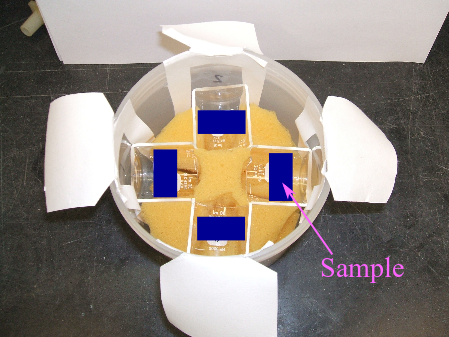
\includegraphics[width=0.4\textwidth]{figures/ripple/MMs/annealing_chamber_topview}
  \quad
  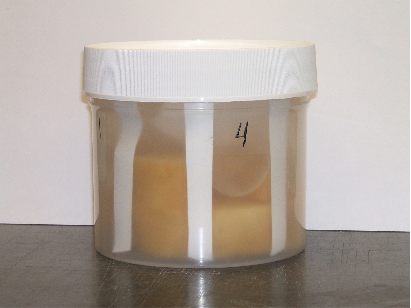
\includegraphics[width=0.4\textwidth]{figures/ripple/MMs/annealing_chamber_sideview}  
  \caption[Pictures of an annealing chamber]{Picture of an annealing chamber.}
  \label{fig:annealing_chamber}
\end{figure}

The sample for the grazing incidence wide angle study was prepared in the same way 
as for low angle study. In order to minimize the geometric broadening, the 
sample was trimmed to 1 mm in width along the beam direction.

The sample for transmission study was deposited on a thin, 35 micron, silicon
wafer, and oriented following the rock and roll procedure \cite{Tristram-Nagle07_MMB}.  
Because the wafer was very fragile, attaching the sample to a sticky 
thing was impossible. Instead, the sample was attached to a plastic cap on 
a small vial with a small amount of heat sink compound at a corner of the 
wafer. The wafer was stable enough for rocking. 

%%%%%%%%%%%%%%%%%%%%%%%%%%%%%%%%%%%%%%%%%%%%%%%%%%%%%%%%%%%%%%%%%%%%%%%%%%%%%%%
\subsection{Instrumental Resolution}\label{sec:instrumental_resolution}
The X-ray scattering experiments were carried out at the Cornell 
High Energy Synchrotron Source (CHESS) G1 station in three different runs
(2011, 2012, and 2013). 
The low angle X-ray scattering (LAXS) data analyzed 
in this thesis were collected in 2013.
The near grazing incidence wide angle X-ray scattering (nGIWAXS) data were also collected
in the 2013 run, but with smaller energy dispersion than in the LAXS experiment.
The transmission wide angle X-ray scattering (tWAXS) data were collected
in the 2011 run. The ripple phase data in the 2012 run were not used
due to low sample quality.
The instrumental resolution in these X-ray experiments depended on the beam
divergence, energy dispersion, and geometric broadening 
as describe in the following subsections.

\subsubsection{Divergence}\label{sec:divergence}
The beam divergence quantifies an angular spread of the incoming X-ray
beam. We estimated the beam divergence by measuring the horizontal and 
vertical beam widths at two known sample-to-detector $S$ distances
with difference $\Delta S$. 
The beam widths were larger at the further distance, which indicated 
that the beam was divergent. 
We calculated the divergence as div = $\Delta B/\Delta S$, where
$\Delta B$ is the difference in beam widths at different $S$ distances.
Table~\ref{tab:beam_divergence} summarizes beam divergence.

\begin{table}[htbp]
  \centering
  \begin{tabular}{cccc}
    \hline
    year & type of  & horizontal & vertical \\
     & experiment & (rad.) & (rad.) \\
    \hline
    2013 & LAXS & $4.2 \times 10^{-5}$ & $1.6 \times 10^{-4}$ \\
    2013 & nGIWAXS & $4.2 \times 10^{-5}$ & $1.6 \times 10^{-4}$ \\
    2011 & tWAXS & $2.5 \times 10^{-5}$ & $5 \times 10^{-5}$ \\
    \hline
  \end{tabular}
  \caption[Beam divergence]{Beam divergence}
  \label{tab:beam_divergence}
\end{table}

\subsubsection{Energy dispersion}\label{sec:energy_dispersion}
A W/B$_4$C multilayer monochromater with energy bandwidth $\Delta E$/$E$ of
$\sim$1.3\% was used in the LAXS and tWAXS experiments. 
The energy of the X-ray beam was 10.55 keV, corresponding to X-ray wavelength 
$\lambda$ of 1.175 \AA, in the LAXS experiment.
To achieve a higher instrumental resolution than that for 
the LAXS experiment, a (111) channel cut silicon monochromator was used for 
the nGIWAXS experiment, which gave $\Delta E/E$ of 0.01\%.
Due to the geometry of the G1 station, the Si monochromator was placed in
the G1 hutch, in series with the multilayer monochromator. 
Table~\ref{tab:energy_dispersion} summarizes energy dispersion.

\begin{table}[htbp]
  \centering
  \begin{tabular}{ccccc}
    \hline
    year & type of & $\Delta E/E$ & $E$ & $\lambda$ \\
     & experiment & (\%) & (keV) & (\AA) \\
    \hline
    2013 & LAXS & 1.5 & 10.55 & 1.175 \\
    2013 & nGIWAXS & 0.01 & 10.55 & 1.175 \\
    2011 & tWAXS & 1.5 & 10.54 & 1.176 \\
    \hline
  \end{tabular}
  \caption[Energy dispersion]{Energy dispersion}
  \label{tab:energy_dispersion}
\end{table}

\subsubsection{Geometric Broadening}\label{sec:geometric_broadening}
The beam footprint on the sample has a finite size and this causes
geometric broadening of diffraction peaks on the CCD detector.

\paragraph{LAXS}
In the LAXS experiment, 
the geometric broadening in the horizontal $x$ direction is simply the 
horizontal beam width for $k=0$ peaks with minor additional broadening
for $k\neq 0$ peaks. Geometric broadening in the vertical $z$ direction
is due to different heights of the sample along the $y$ direction of the beam 
at non zero angle of incidence $\omega$. It is given approximately by
$w_s\tan\theta$, where $w_s$ is the sample width along the $y$
direction and $\theta$ is the scattering angle.
The beam shape, measured through a semi-transparent 200 $\mu$m thick
molybdenum (Mo) beam stop, is shown in Fig.~\ref{fig:ripple_lr_beamx}
and \ref{fig:ripple_lr_beamz}.
The horizontal beam width was 1.7 pixels (0.12 mm). The vertical beam
height was approximately 1 mm, tall enough to cover the entire sample
if the sample was tilted between 0\textdegree\ and 11.5\textdegree. 
The sample was rocked
during X-ray exposure between -1.6\textdegree\ and 7\textdegree\ 
in order to observe many diffraction peaks in one data collection.

\begin{figure}[p]
  \centering
  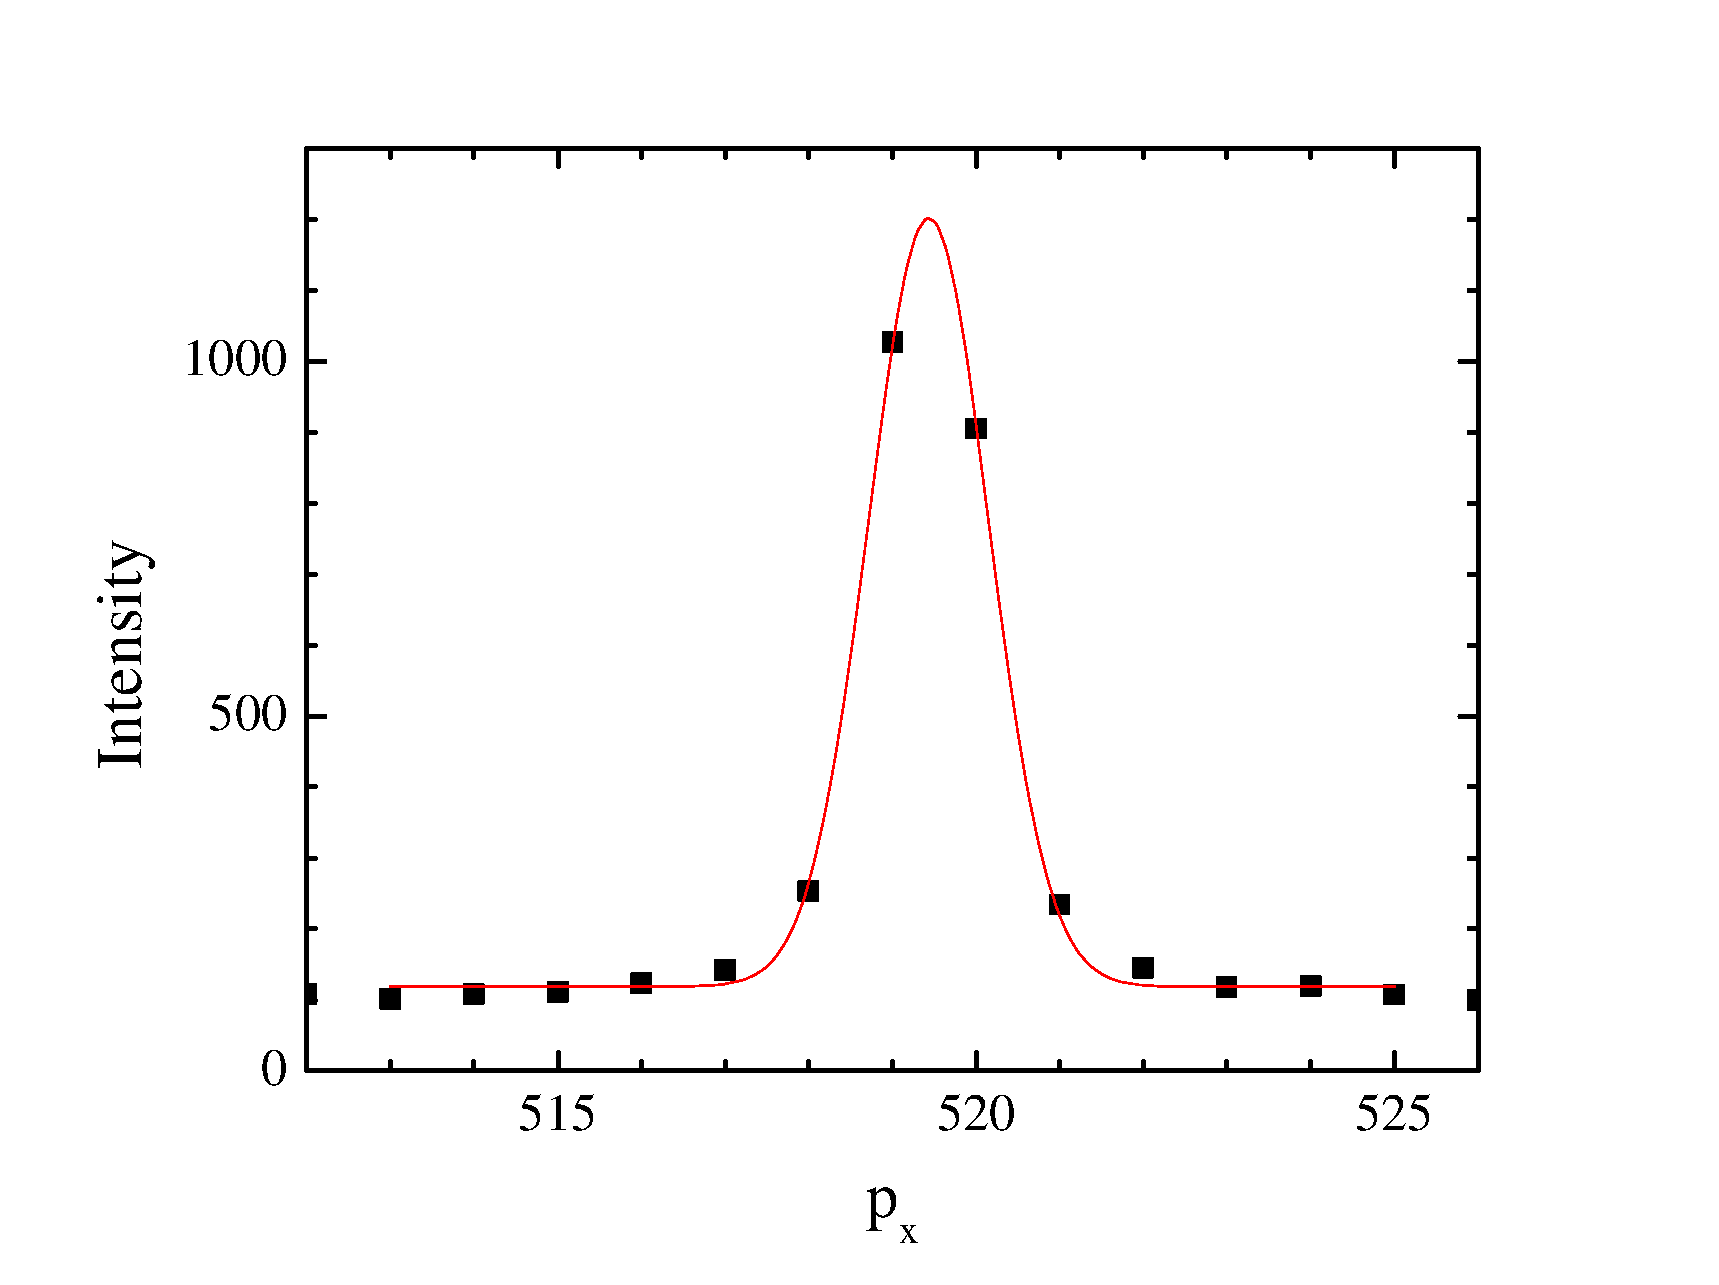
\includegraphics[width=0.7\textwidth]{figures/ripple/MMs/laxs/beamx_lr}
  \caption{The horizontal profile of the beam used in the 2013 low resolution study.
  Each pixel was 0.07113 mm, which gave a CCD angular resolution $\Delta\theta$ of 
  0.0057\textdegree, corresponding to $\Delta q=0.0011$ \AA$^{-1}$ at the 
  sample to detector distance of 359.7 mm. 
  The beam FWHM = 1.7 pixels, giving $\Delta\theta = 0.010$\textdegree\ or
  $\Delta q= 0.0019$ \AA$^{-1}$.}
  \label{fig:ripple_lr_beamx}
\end{figure}

\begin{figure}[p]
  \centering
  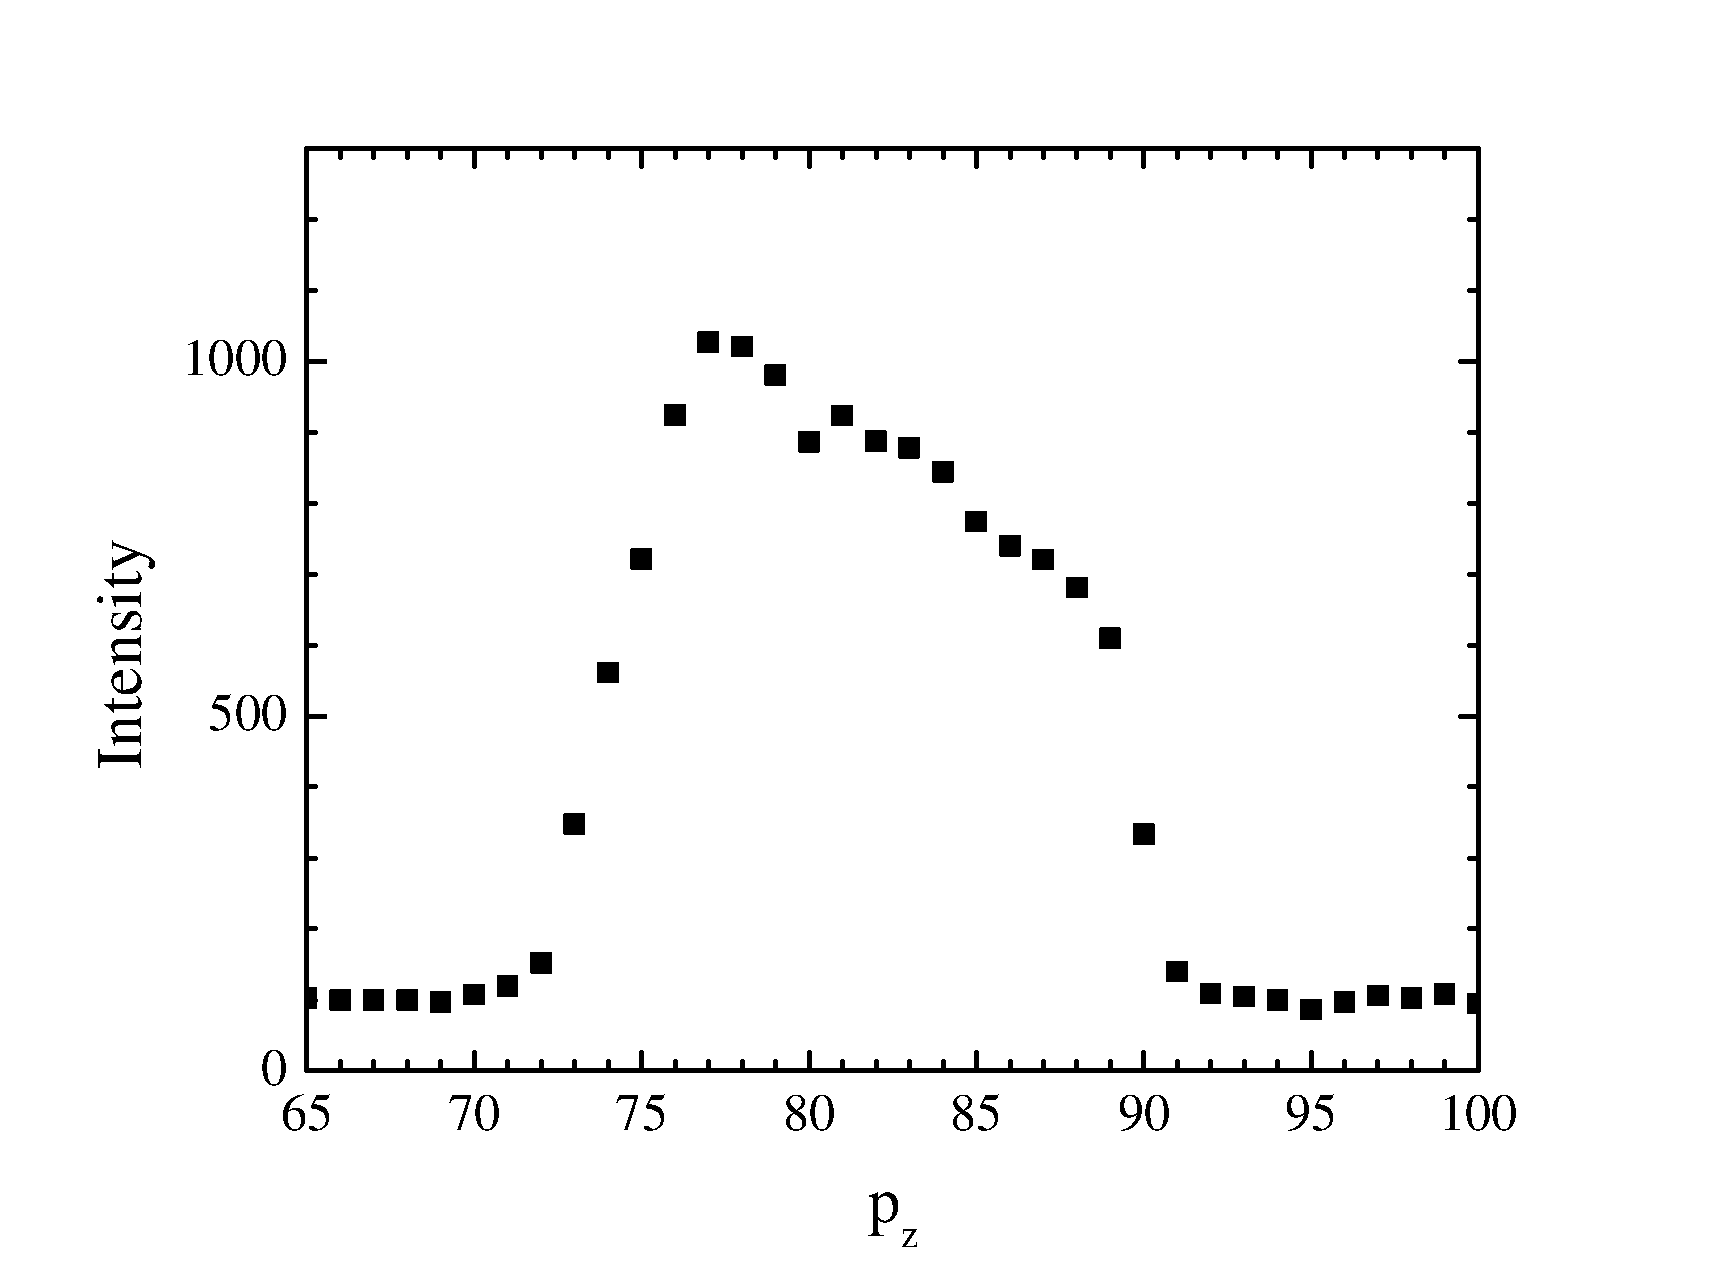
\includegraphics[width=0.7\textwidth]{figures/ripple/MMs/laxs/beamz_lr}
  \caption{The vertical profile of the beam used in the 2013 low resolution study.
  The beam height = 15 pixels = 1.1 mm.}
  \label{fig:ripple_lr_beamz}
\end{figure}

\paragraph{nGIWAXS}
In the nGIWAXS experiment, 
the horizontal geometric broadening was due to the
sample width along the beam direction and the horizontal beam width.
From the geometry of the experiment shown in Fig.~\ref{fig:geometric_broadening}, 
the geometric broadening $\Delta x$ can be estimated,
assuming simple additivity,
\[
\Delta x = \Delta x_\textrm{beam} + w_\textrm{s}\tan(2\theta),
\] 
where $\theta$ is the in-plane scattering angle.
The total scattering angle $2\theta$ for the ripple WAXS was approximately 
16\textdegree. 
To minimize the contribution to $\Delta x$ from the sample, 
the sample was trimmed to $w_s$ = 1 mm along the beam direction. 
This width was chosen because (1) I could not trim more
without a more sophisticated device than a simple razor blade, (2) a very
narrow sample would be a weak scattering body, and (3) disordering effect from 
the sample edge might become too significant to ignore. 
Given the above reasons and due to limited availability
of synchrotron beam time, I considered a 1 mm width to be reasonable.
The horizontal beam width was 3.7 pixels (0.26 mm) as shown in
Fig.~\ref{fig:nGIWAXS_beamx}.
With these experimental parameters, 
the resolution was estimated to be $\Delta x = 0.57$ mm = 8 pixels, 
which would be the unresolved width of an intrinsically infinitely sharp 
wide angle peak.
Indeed, the measured width of the (2, 0) Bragg peak in the gel \LbetaI\ phase
was 8 pixels as will be shown in Fig.~\ref{fig:gel_phase}.
The sample to detector distance were 220.6 mm, measured using silver behenate.
Then, the minimum peak width measured in $q$-space would be
$\Delta q \approx 0.014$ \AA$^{-1}$. The vertical geometric broadening 
was negligible because the sample width $w_s$ was narrow and scattering
of interest occurred at small $q_z$.

\begin{figure}[htbp]
  \centering
  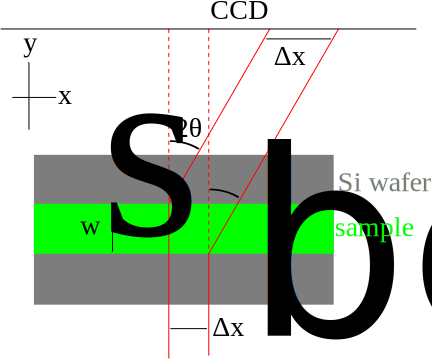
\includegraphics[width=0.5\textwidth]{figures/ripple/MMs/waxs/geometric_broadening}
  \caption{In-plane geometric broadening due to the sample width $w_s$ and the beam width $\Delta x_\textrm{beam}$.
  A top view of the sample (green) on the Si wafer (gray) and the
  incoming and diffracted X-rays (bounded by red solid lines)
  are shown. The total in-plane scattering
  angle is labeled $2\theta$, and 
  the geometric broadening on the CCD is $\Delta x$.}
  \label{fig:geometric_broadening}
\end{figure}

\begin{figure}[htbp]
  \centering
  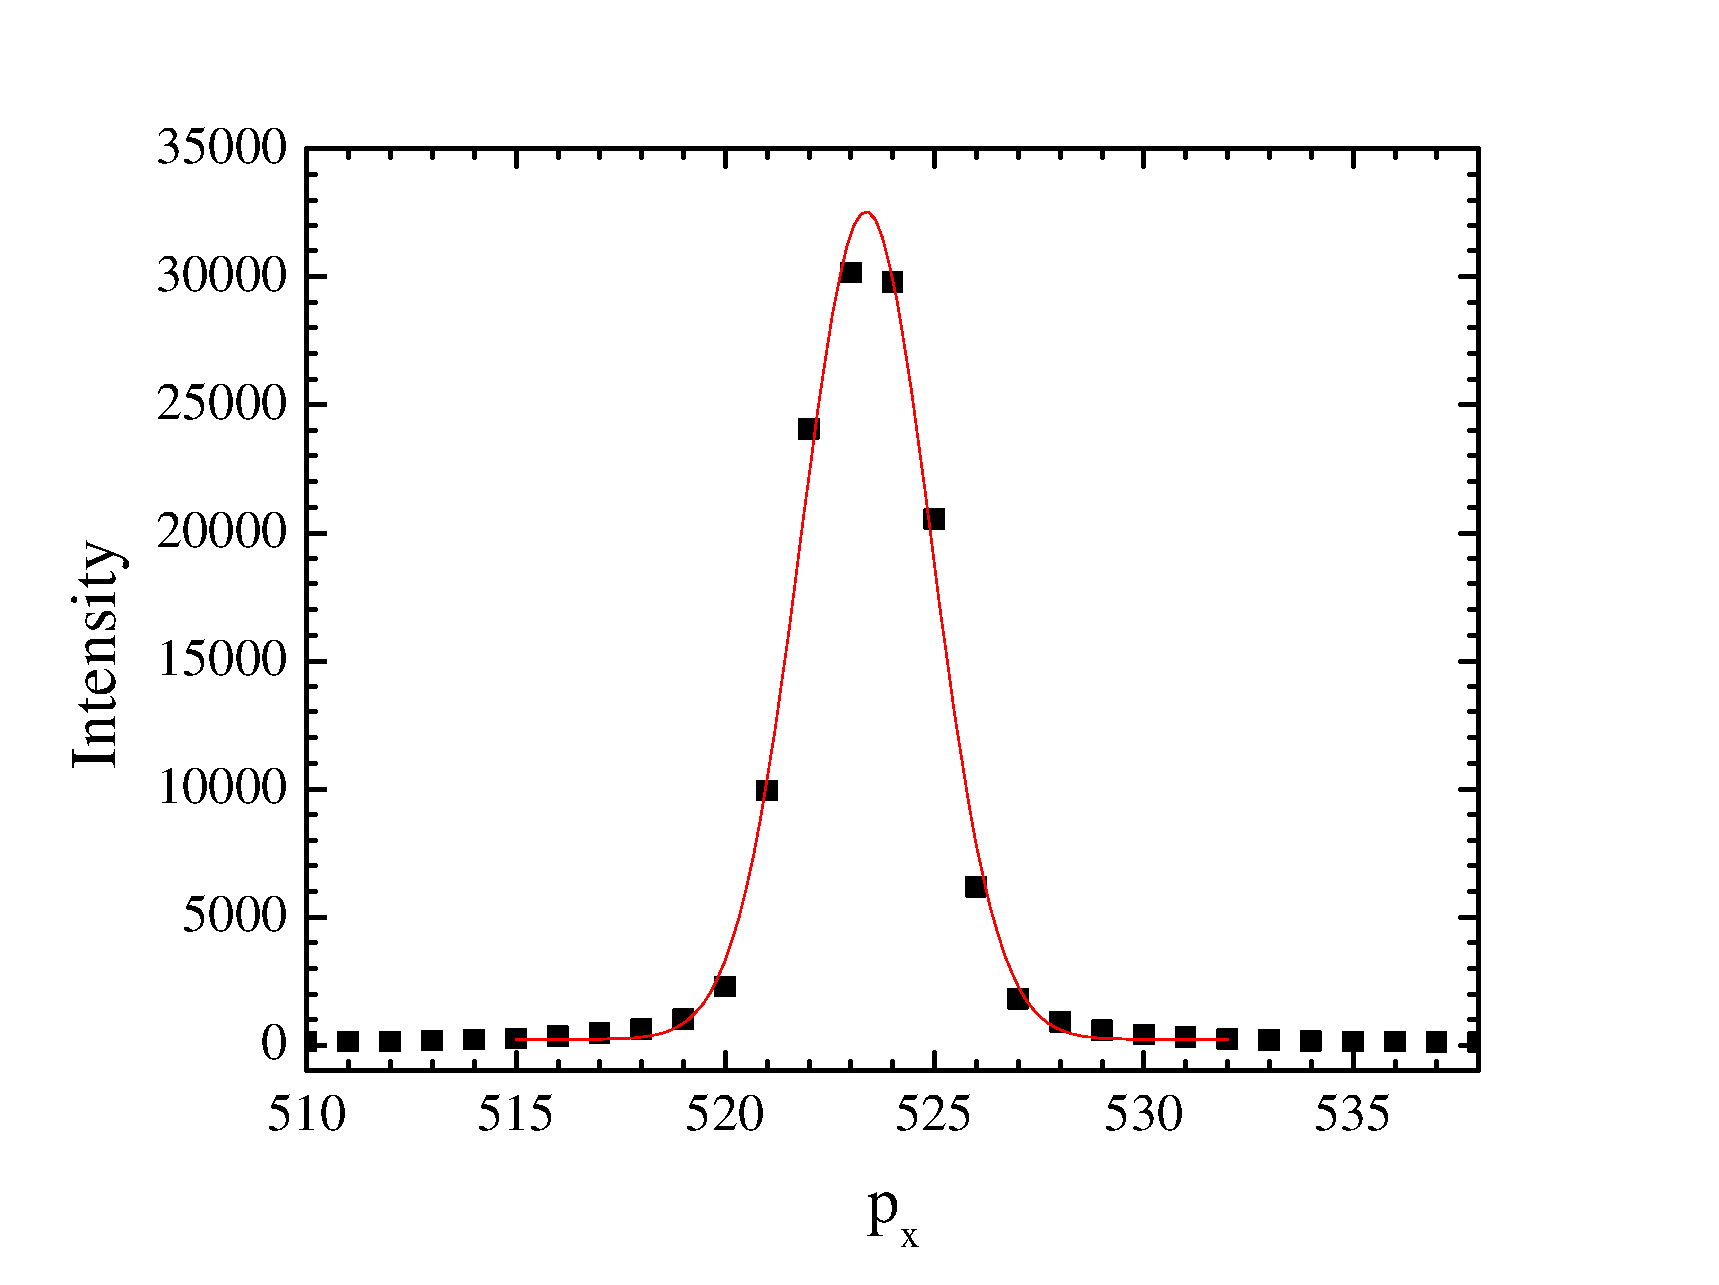
\includegraphics[width=0.7\textwidth]{figures/ripple/MMs/waxs/beamx_hr}
  \caption{The horizontal profile of the beam used in the 2013 high resolution 
  experiment. The CCD angular resolution $\Delta\theta$ = 0.0092\textdegree\,
  corresponds to $\Delta q$ = 0.0017 \AA$^{-1}$ at the sample to detector
  distance of 220.6 mm. The beam FWHM = 3.7 pixels = 0.26 mm, giving
  $\Delta\theta$ = 0.034\textdegree\ or $\Delta q$ = 0.0063 \AA$^{-1}$. }
  \label{fig:nGIWAXS_beamx}
\end{figure} 

\begin{figure}[htbp]
  \centering
  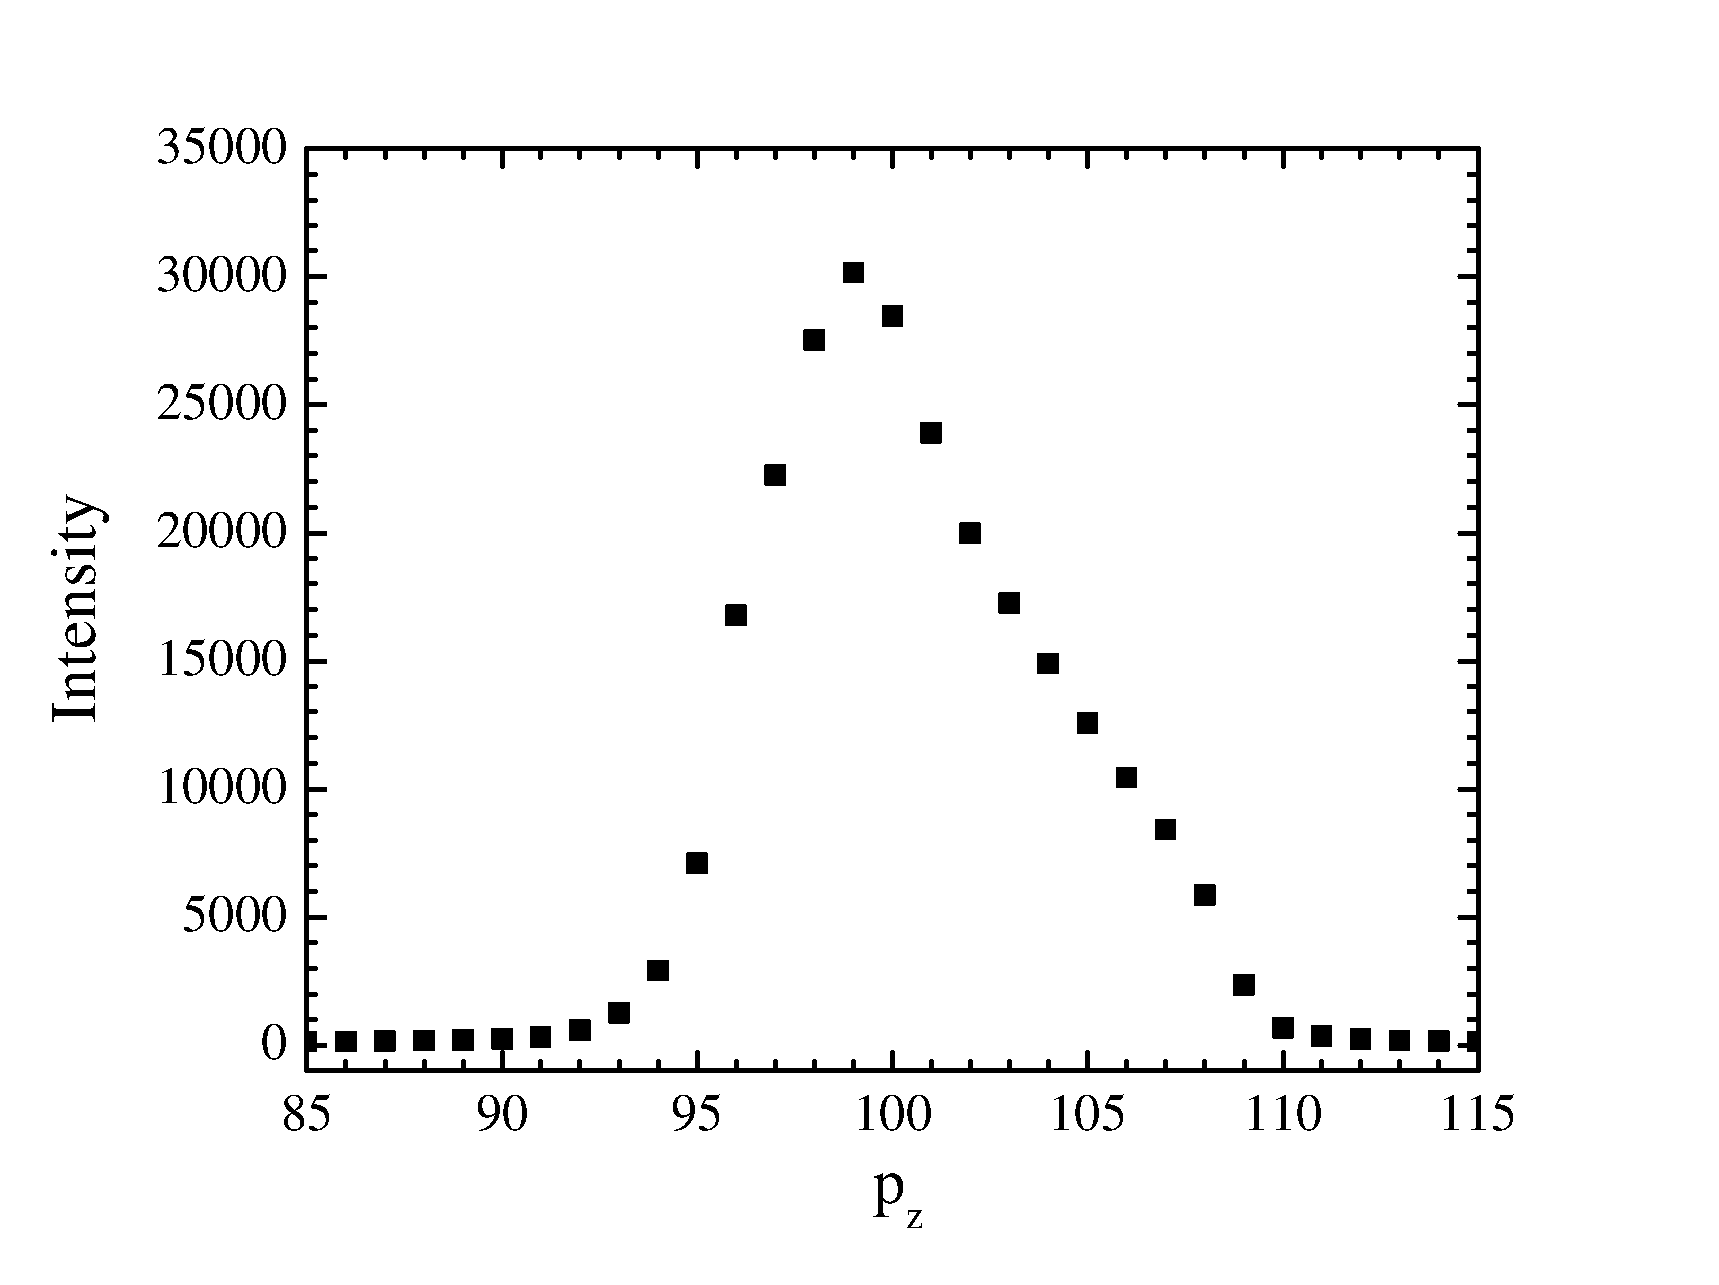
\includegraphics[width=0.7\textwidth]{figures/ripple/MMs/waxs/beamz_hr}
  \caption{The vertical profile of the beam used in the 2013 high resolution experiment.
  The beam height = 9 pixels = 0.64 mm.}
  \label{fig:nGIWAXS_beamz}
\end{figure} 

\paragraph{tWAXS}
In transmission WAXS, 
geometric broadening in both $x$ and $z$ directions was non-negligible.
To calculate the broadening, let us assume that the beam has a rectangular
cross section with its height $Y_b$ and width $X_b$ as shown in Figure 
\ref{fig:gb_trans1}. When the sample is tilted by $\omega$, X-rays emerging 
from the top edge of the sample travel extra distance compared to the distance 
that X-rays from the bottom edge of the sample travel. This, then, leads to 
distortion of the scattered beam; namely, the scattered beam will appear on 
the CCD screen as a parallelogram as shown in Figure 
\ref{fig:gb_trans1}. 
Figure \ref{fig:gb_trans2} shows the top- and sideview of the 
projection of the beam on the sample. From simple geometry, it can be shown 
that $a=Y_b/\tan\omega$, $b=aX/(2S)$, $c=aZ/(2S)+Y_B/2$, and $B=\tan^{-1}(Z/S)$. 
Since $H=2c$ and $W=2b$, $H$ and $W$ in Figure~\ref{fig:gb_trans3} are 
given by
\begin{align}
	H &= Y_b\left(1+\frac{Z}{S\tan\omega}\right)\\
	W &= Y_b\frac{X}{S\tan\omega}.
\end{align}
The sample to detector distance $S$ was 158.6 mm, giving an angular
CCD resolution of 0.013\textdegree/pixel, 
or 0.0024 \AA$^{-1}$/pixel.
The observed wide angle peak was at $(X,Z)$=(44.0 mm, 15.5 mm). 
The beam width and height were both 0.2 mm = 2.8 pixels.
With this setup, $W$ = 0.7 pixels and $H$ = 3.1 pixels. 
Therefore, the distorted shape of the diffraction peak was negligible.
Table~\ref{tab:geometric_broadening} summarizes geometric broadening for
our experiments.

\begin{figure}[htbp]
  \centering
  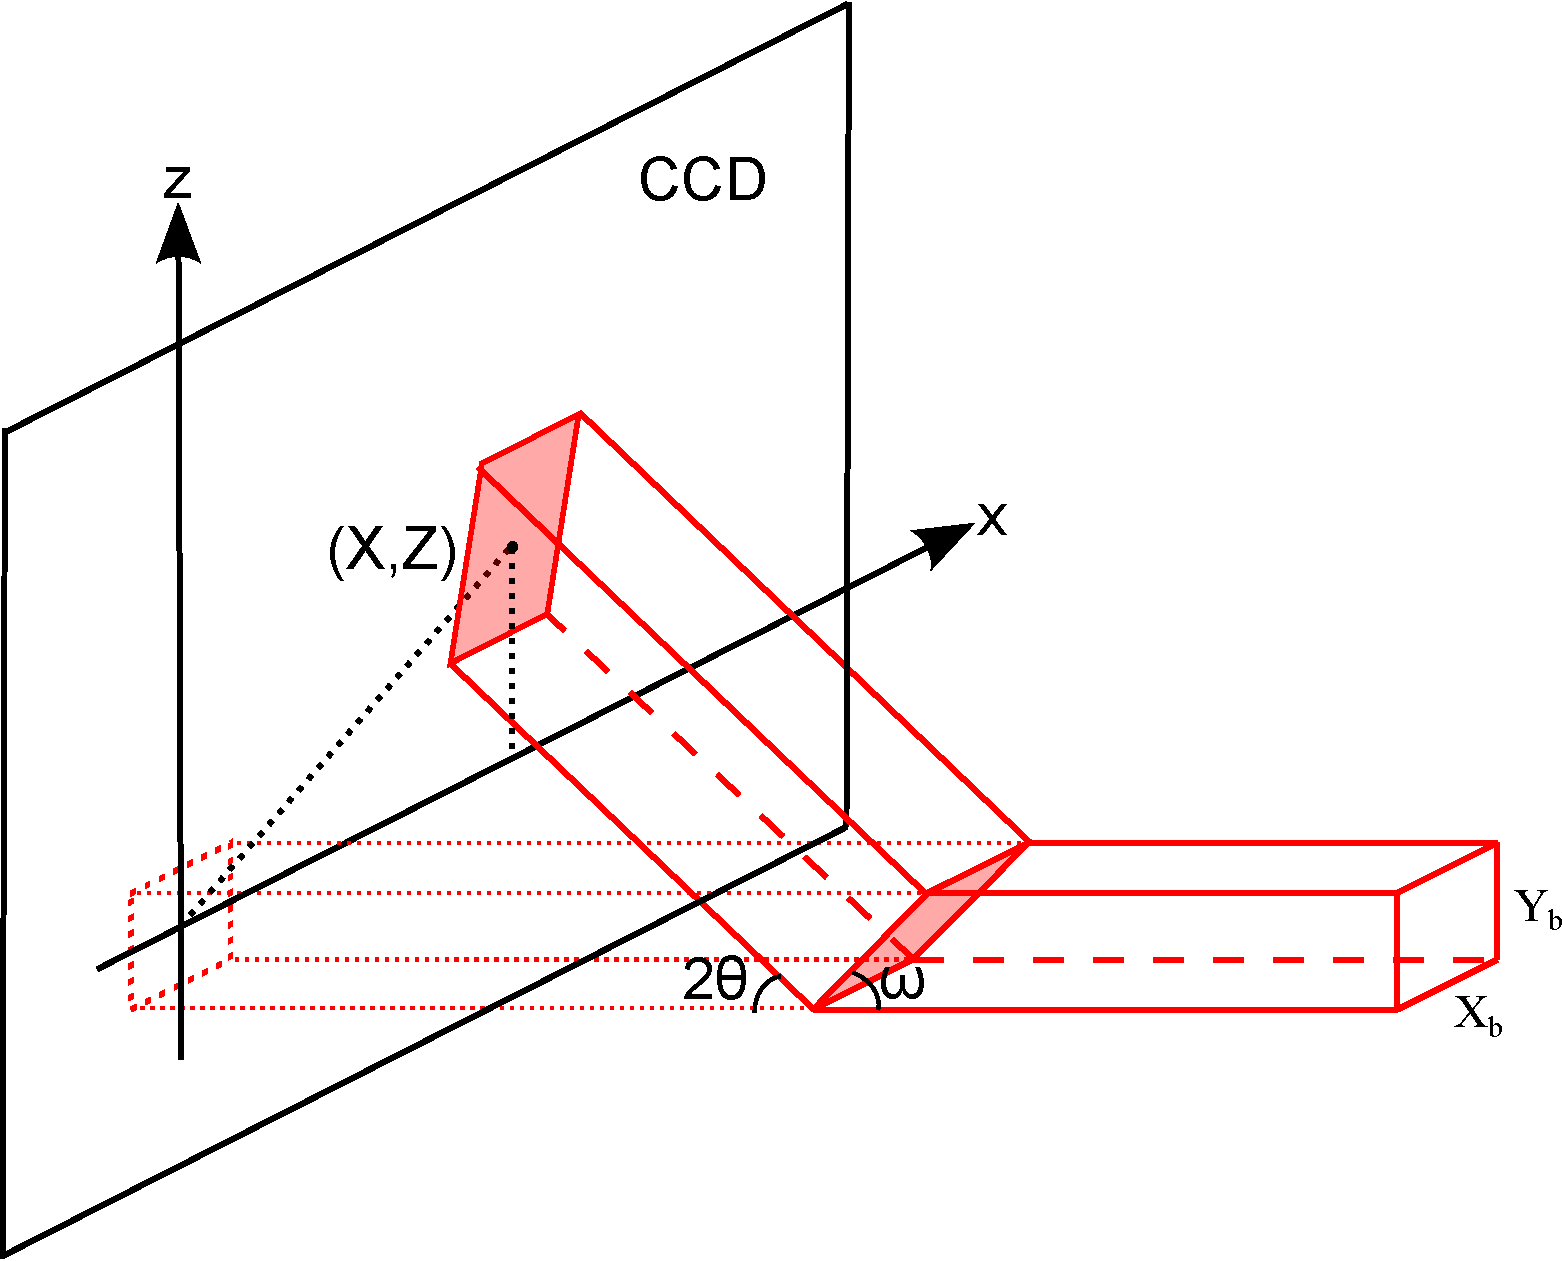
\includegraphics[width=0.5\textwidth]{figures/ripple/MMs/transmission/geometric_broadening1}
  \caption[Geometric broadening in tWAXS]{Geometric broadening in tWAXS. 
  The cross section of the incoming X-ray with the sample and the CCD 
  detector are both shaded in red. The sample is tilted by $\omega$.
  The red dots show the transmitted beam. The incoming beam is rectangular
  but upon scattering appears as a parallelogram on the CCD.}
  \label{fig:gb_trans1}
\end{figure}

\begin{figure}[htbp]
  \centering
  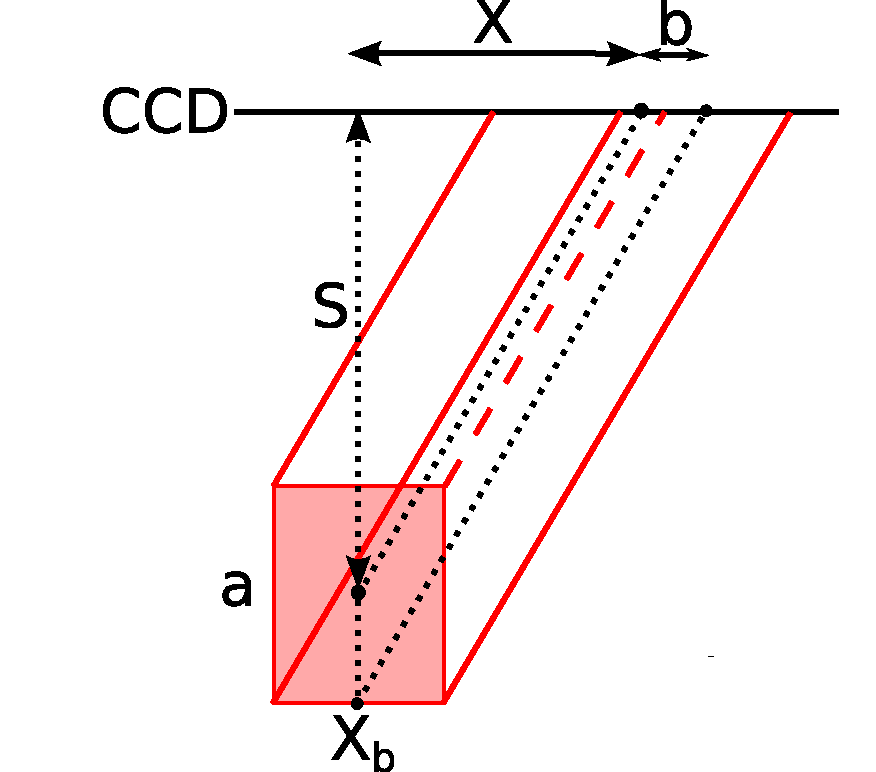
\includegraphics[width=0.45\textwidth]{figures/ripple/MMs/transmission/geometric_broadening2}
  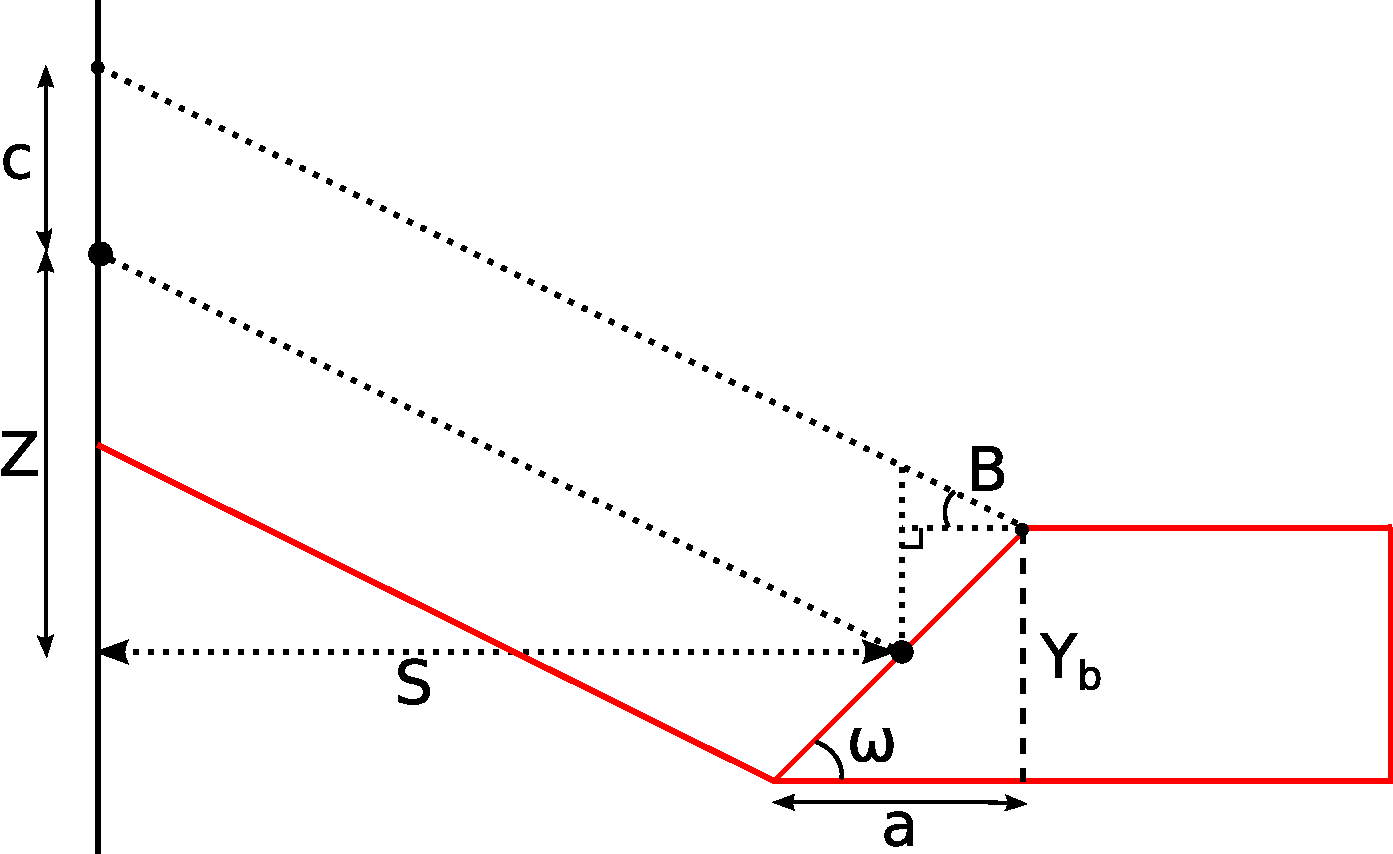
\includegraphics[width=0.45\textwidth]{figures/ripple/MMs/transmission/geometric_broadening3}
  \caption[Top and side view of the beam on the sample in tWAXS]{Top and side 
  view of the beam on the sample in tWAXS. The cross section of the incoming X-ray 
  with the sample is shaded in red. 
  $X_b$ and $Y_b$ are the beam width and height, respectively. 
  $S$ is the sample to detector distance. 
  $(X,Z)$ is a  
	position of the center of the scattered beam on the detector with respect 
	to the center of the transmitted beam as shown in 
	Figure~\ref{fig:gb_trans1}.}
  \label{fig:gb_trans2}
\end{figure}

\begin{figure}[htbp]
  \centering
  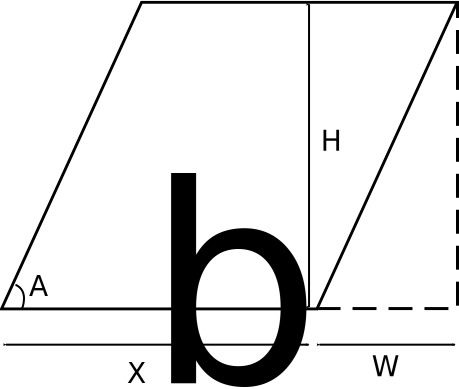
\includegraphics[width=0.3\textwidth]{figures/ripple/MMs/transmission/geometric_broadening4}
  \caption{Projection of rectangular beam on the detector. Scattered beam
  appears as a parallelogram on the CCD.}
  \label{fig:gb_trans3}
\end{figure}

\begin{table}[p]
  \centering
  \begin{tabular}{cccccc}
    \hline
    year & type of & horizontal & horizontal & vertical & vertical \\
     & experiment & (pixels) & (\AA$^{-1}$) & (pixels) & (\AA$^{-1}$) \\
    \hline
    2013 & LAXS & 1.7 & 0.0019 & 6.6$q_z$ & 0.0072$q_z$ \\
    2013 & nGIWAXS & 8 & 0.014 &  & \\
    2011 & tWAXS & 2.8 & 0.0067 & 3.1 & 0.0074 \\
    \hline
  \end{tabular}
  \caption{Geometric broadening}
  \label{tab:geometric_broadening}
\end{table}

\newpage
\subsection{Low Angle X-ray Scattering Experiment}\label{sec:LAXS_method}
The X-ray beam for the low angle X-ray scattering (LAXS) experiment 
was set up by the station scientist, Dr. Arthor Woll.
We chose the sample to detector distance to be 359.7 mm, measured by indexing
silver behenate Bragg peaks. The D-spacing of silver behenate is known to be
58.367 \AA.

Occasionally, sheets of molybdenum (Mo), each nominally 25 $\mu$m were 
used to attenuate the incoming beam. 
These sheets had been installed in the G1hutch by Dr. Woll upstream of our 
sample chamber.
The attenuation length $\mu$ of 10.55 keV X-ray in Mo is 13.74 $\mu$m \cite{ref:cxro}.
%8 keV X-ray in Mo is 6.433 $\mu$m
For a 25 $\mu$m thick Mo attenuator, the attenuation factor is calculated to be
$[\exp(-25/13.74)]^{-1} = 6.2$. The exact attenuation factor was determined
by comparing X-ray images collected with and without the attenuator, 
shown in Fig.~\ref{fig:olddopc}.
The attenuation factor of the nominally 25 $\mu$m thick Mo was found to 
be 6.9 for the wavelength used (1.175 \AA), indicating an actual thickness
of ~27 $\mu$m. 

\begin{figure}[jtbp]
  \centering
  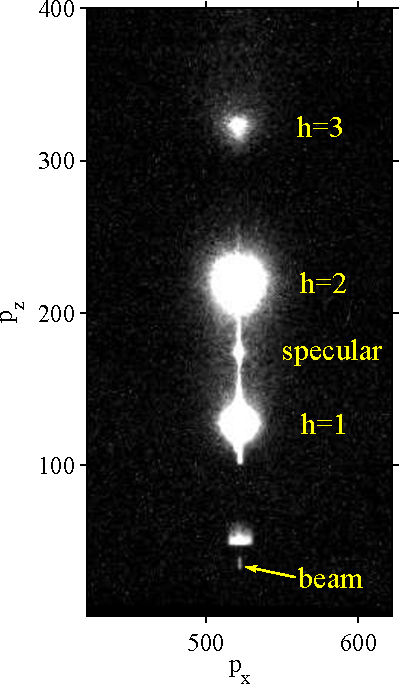
\includegraphics[width=0.35\textwidth]{figures/ripple/MMs/laxs/olddopc045_labels}
  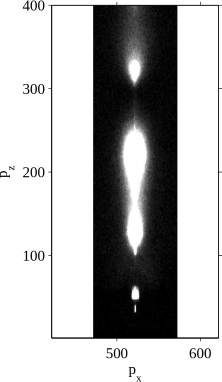
\includegraphics[width=0.35\textwidth]{figures/ripple/MMs/laxs/olddopc044}
  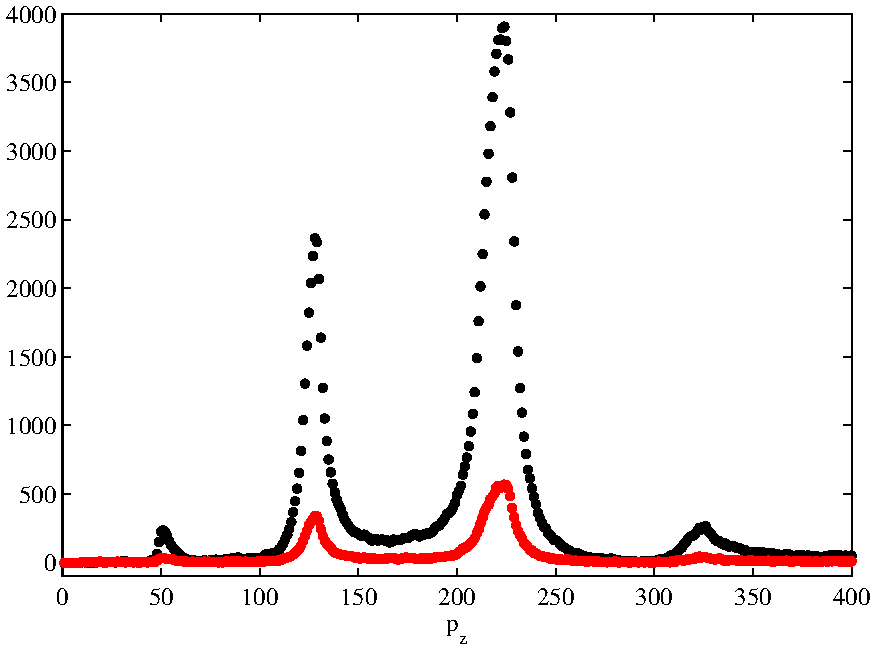
\includegraphics[width=0.45\textwidth]{figures/ripple/MMs/laxs/attenuator1}
  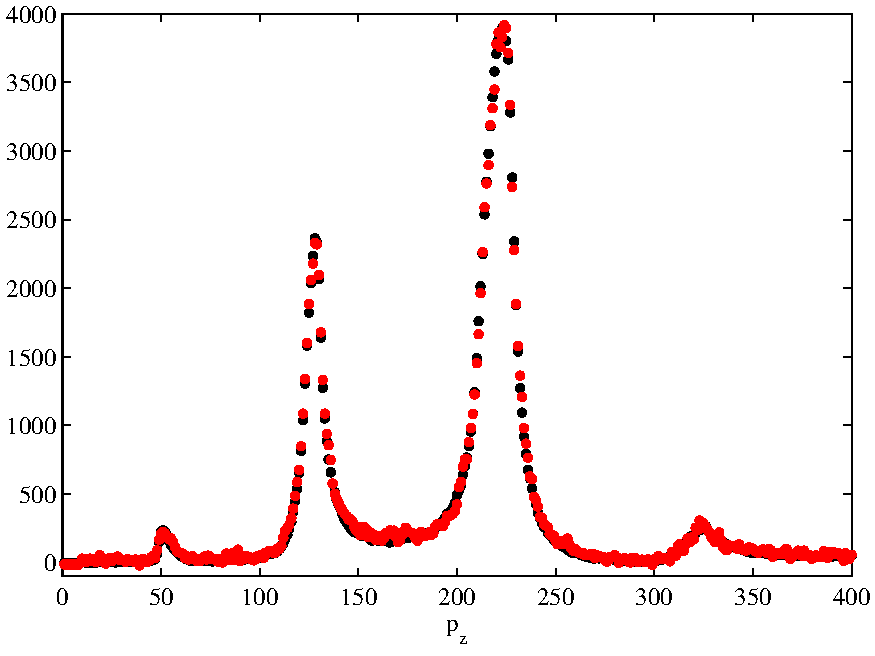
\includegraphics[width=0.45\textwidth]{figures/ripple/MMs/laxs/attenuator2}
  \caption{(top panels) CCD images of X-ray scattering taken with (left) and without 
  (right) a nominally 25 $\mu$m thick Mo attenuator. These data were taken 
  at a fixed angle of incidence $\omega=0.8$\textdegree. The sample was an oriented film of 
  DOPC:DOPE (3:1) in the fluid phase at 37 \textcelsius. The wavelength
  was 1.175 \AA, the same as the one used for the ripple phase experiment.
  The same gray scale is used in both images. 100 pixel =  0.11 \AA$^{-1}$ in $q$. 
  A small dot located about $(p_x,p_z)=(520,170)$ between the first and second orders is 
  a specular reflection from the substrate. The exposure times were 1 second. 
  (bottom panels) Vertical $p_z$ slices of the X-ray images shown in the top panels (left).
  The scattering intensity measured with the attenuator (red solid circles) 
  was multiplied by a factor of 6.9 and compared to the intensity measured 
  without the attenuator (black solid circles, right).}
  \label{fig:olddopc}
\end{figure}

Sheets of Mo were also used as a semi-transparent beam stop downstream of the 
sample, just 
outside the hydration chamber, to attenuate the beam and strong orders.  
To avoid saturation of CCD pixels by
the very intense beam of $\sim$10$^{11}$ photons/mm$^2$/second, 200 or 225 $\mu$m 
were used depending on the exposure time.  Also, for long exposures 100 or 200 
$\mu$m were used to attenuate strong lower orders.  The longest exposure times 
were typically 60 or 120 seconds (doubled for dezingering), varying somewhat for 
different runs.

A few Bragg peaks in the low angle X-ray scattering of the ripple phase
were very strong, leading to saturation of CCD pixels for data collection
with a long exposure time. 
In order to probe a wide range of $q$-space, three images were taken:
1) a short, one second exposure with a nominally 25 micron 
molybdinum attenuator installed in the upstream of the sample to reduce the 
intensity
of the incoming X-ray beam so that the intense (1,0) reflection did not 
saturate the CCD, 2) one second exposure without the beam attenuator,
and 3) 60 second exposure with a 100 $\mu$m Mo strip attenuating the very 
intense 
(1,0) and (2,0) peaks. The latter two exposures are shown in 
Fig.~\ref{fig:ripple_laxs_images}. 
Then, the integrated intensity of the (1,0) reflection was measured
from the first image. This value was multiplied by 6.9 to account for the beam
attenuation and then multiplied again by 60 to scale with intensities obtained 
at the longest exposure time. 
The intensity of (2,0) and (2,-1) were measured from the second image, also
multiplied by 60 to account for the shorter exposure time. The intensities of
the rest of the observed peaks were measured from the third image.

The integrated intensity of each peak was obtained using the Nagle lab tview
software developed by Dr. Yufeng Liu \cite{Liu03} by putting a box around a
peak and summing up the intensity in those pixels that fall inside the box.
The background scattering was estimated by measuring the intensity in pixels
near the peak but not containing any peak tail. The choice of box size was 
made according to the width of each peak. Because of mosaic spread in the sample,
the peaks were wider for higher orders. 
Consequently, the box was made wider for higher
orders. The box size was chosen so that approximately 80\% of the peak intensity
was counted toward the integrated intensity.

\subsection{Near Grazing Incidence Wide Angle X-ray Scattering nGIWAXS}\label{sec:nGIWAXS_method}
The high resolution wide angle X-ray scattering (WAXS)
experiment was also carried out at the G1 station. 
A channel cut silicon monochromator was set up by the G1
station scientist, Arthur Woll, and the assistant scientist, Dr. Robin Baur.
Wide angle X-ray scattering was collected at an incident angle $\omega=$ 
0.2\textdegree. 
The total external reflection from an air-lipid interface occurs approximately 
at 0.1\textdegree\ and 0.17\textdegree\ for air-silicon interface, 
so 0.2\textdegree\ is not quite grazing incidence.
Grazing incidence usually implies that the incident angle is less than the 
critical angle for a total external reflection.
Therefore, 0.2\textdegree\ is called near grazing incidence (nGI) in this thesis.
The background scattering was collected at $\omega$ = -0.2\textdegree. Subtraction
of the negative angle data from the positive angle data resulted in 
a clean sample scattering image as will be shown in 
Fig.~\ref{fig:waxs_data_reduction}.

%S1L = 153.6 mm, S1H = 220.6 mm, and S2 = 359.7 mm

\subsection{Transmission Wide Angle X-ray Scattering tWAXS}\label{sec:tWAXS_method}
These experiments were also carried out at the G1 station.
The incident angle $\omega$ was set to -45\textdegree\ for transmission data
collection (see Fig.~\ref{fig:holder_schematic}). 
A 35 $\mu$m thick silicon substrate absorbs 10.5 keV X-rays 
by only 20\%\ \cite{ref:cxro}, so most of the incoming X-rays penetrated
the thin substrate and none of the scattered X-rays were absorbed by the 
substrate.  This is a distinct advantage of tWAXS compared to nGIWAXS because 
reflections with small values of $q_z$ are not attenuated compared to those 
with large values of $q_z$.
 
The sample holder for tWAXS is shown in Fig.~\ref{fig:holder_picture} and a 
schematic is shown in Fig.~\ref{fig:holder_schematic}.  Unfortunately, it was not 
possible to design this sample holder so that the axis of rotation of the 
motor in the sample chamber coincided with the sample as it does for LAXS and 
nGIWAXS experiments.  This meant that the sample to detector distance varied 
as $\omega$ was varied. To accurately
measure the sample to detector distance, low angle scattering from a 
silver behenate (AgBe) sample was collected
at a fixed $\omega$. Due to large mosaic spread of the AgBe sample, many orders were
visible. While the relative intensity of each order was inaccurate, 
the positions of peaks were the same as those observed with a rotating sample.
To measure the D-spacing of the sample, $\omega$ was set to 1\textdegree.
The sample to detector distance was measured to be 174.7 mm 
at $\omega$ = 0\textdegree.
From the sample holder geometry shown in Fig.~\ref{fig:sgeometry},
the sample to detector distance was estimated to be 
158.6 mm at $\omega=45$\textdegree.

To level the sample, 
the sample was first leveled coarsely by watching the sample scattering. When
$\omega$ was negative, much of the incoming beam was absorbed by the 
flat substrate, yielding weak sample scattering. When $\omega$ became 
positive, sample scattering was strong. With this procedure, 
we leveled the sample with an uncertainty of $\pm 0.2$\textdegree. We
then measured the beam intensity at various sample heights 
as a function of $\omega$. 
The sample was 
level when the beam intensity had the narrowest dip as the sample
was moved vertically through the beam.

Background scattering was collected by replacing the sample with a bare 
wafer. The bare wafer was not placed exactly at the same location
as the sample, which gave slightly different background scattering.
This only affected the background subtraction near the beam. 
The wide angle scattering was not affected by
this inexact placement of the bare wafer. 
\newpage
\begin{figure}[htbp]
  \centering
  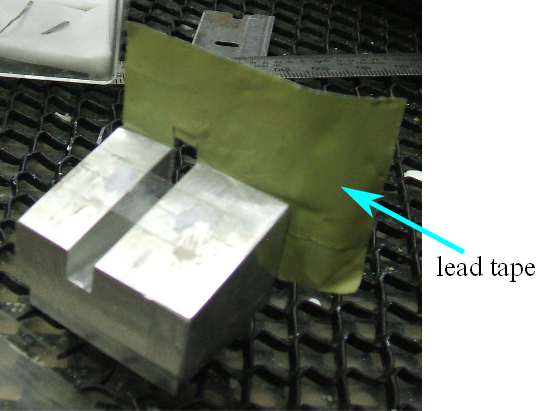
\includegraphics[width=0.45\textwidth]{figures/ripple/MMs/transmission/sample_holder1}
  \caption{Picture of the sample holder looking from above. A lead tape was
  attached to the back of the sample holder to help reduce the background 
  scattering, typically coming from the air gap between the flightpath snout
  and the mylar window of the chamber.}
  \label{fig:holder_picture}
\end{figure}

\begin{figure}[htbp]
  \centering
  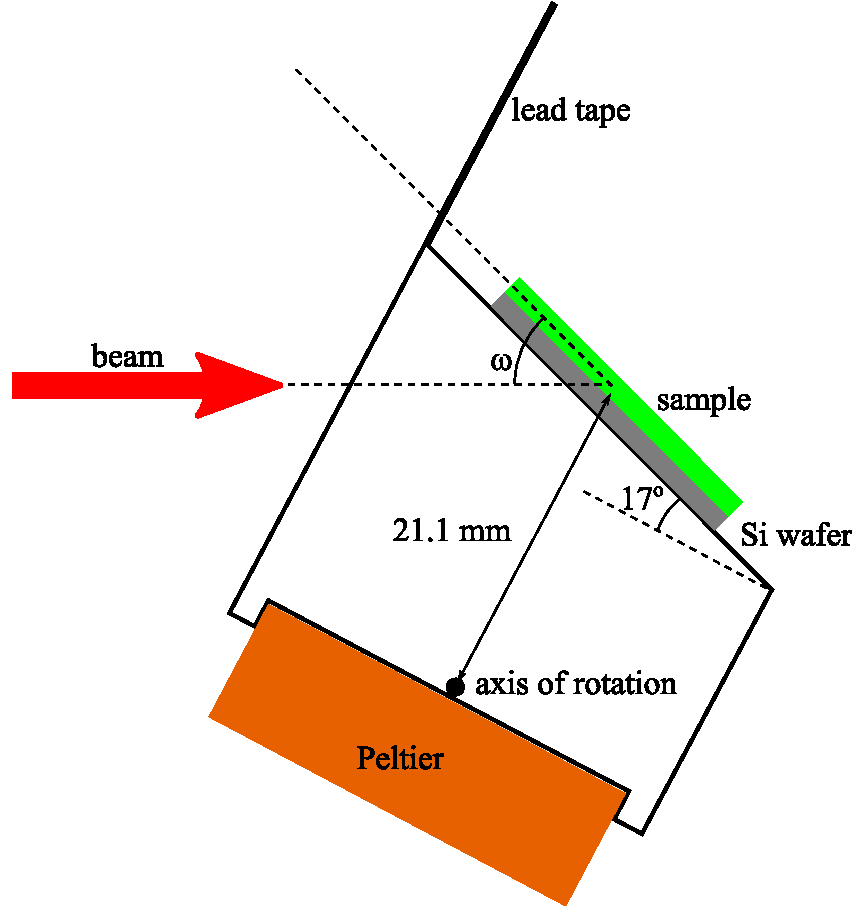
\includegraphics[width=0.55\textwidth]{figures/ripple/MMs/transmission/holder_side}
  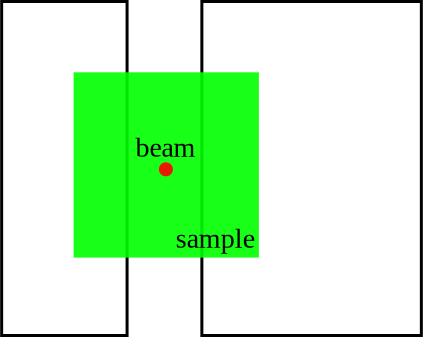
\includegraphics[width=0.35\textwidth]{figures/ripple/MMs/transmission/holder_top}
  \caption{Schematics of the sample holder in the transmission mode.
  Side (left) and top (right) views are shown. The thickness of the Si wafer
  = 35 $\mu$m. The thickness of the sample $\approx$ 10 $\mu$m. The
  distance between the axis of rotation and sample = 21.1 mm.}
  \label{fig:holder_schematic}
\end{figure}

\begin{figure}[htbp]
  \centering
  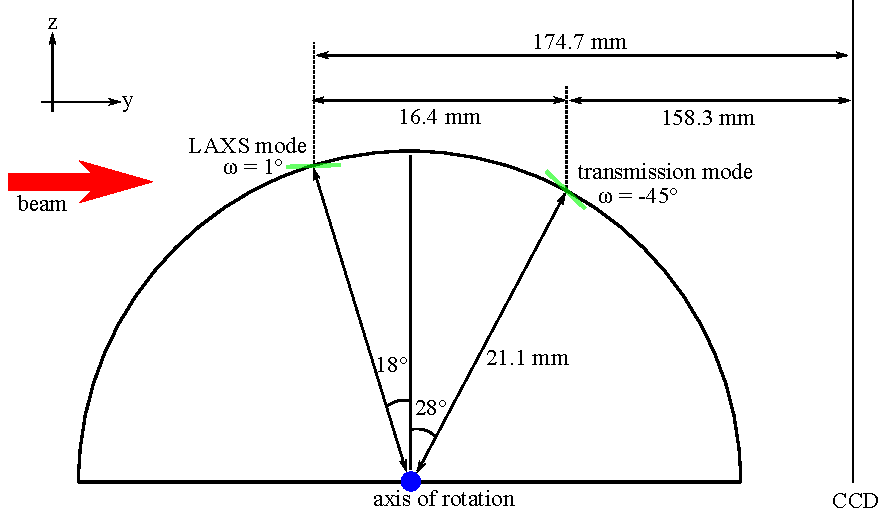
\includegraphics[width=0.8\textwidth]{figures/ripple/MMs/transmission/sgeometry}
  \caption{Circular path followed by the sample 
  as the angle of incidence $\omega$ was changed. The sample to detector distance and 
  $D$-spacing of the sample were measured in the LAXS mode, where $\omega$ = 1\textdegree. WAXS images
  were collected at the transmission mode, where $\omega$ = -45\textdegree. 
  The $z$ position of the sample was
  slightly higher at the LAXS mode than at the transmission mode, so the 
  sample holder was vertically shifted for different modes.}
  \label{fig:sgeometry}
\end{figure}
\newpage
%%%%%%%%%%%%%%%%%%%%%%%%%%%%%%%%%%%%%%%%%%%%%%%%%%%%%%%%%%%%%%%%%%%%%%%%%%%%%%%
\subsection{Sample q-space}\label{sec:sample_q-space}
The incoming and outgoing wavevectors of the x-ray beam in Fig.~\ref{fig:laxs_setup}
are given by
\begin{equation}
  \kin = \frac{2\pi}{\lambda} \yhat, \quad
  \kout = 
    \frac{2\pi}{\lambda} \left( 
      \sin 2\theta \cos\phi \, \xhat
      + \cos 2\theta \, \yhat
      + \sin 2\theta \sin\phi \, \zhat 
    \right),
  %\label{eq:kinkout}
\end{equation}
where $\lambda$ is the wavelength of x-ray, $2\theta$ is the total scattering
angle, and $\phi$ is the angle measured from the equator on the detector. 
The scattering vector (also called
momentum transfer vector) is
the difference between $\kin$ and $\kout$,
\begin{align}
  \mathbf{q} &= \kout - \kin \nonumber \\
             &= q \left( 
                  \cos\theta\cos\phi \, \xhat - \sin\theta \, \yhat
                  + \cos\theta\sin\phi \, \zhat
                \right),
  \label{eq:q_vector}
\end{align}
where $q=4\pi\sin\theta/\lambda$ is the magnitude of the scattering vector. 
When the sample is rotated by $\omega$ about the lab x-axis in the clockwise 
direction as shown in Fig.~\ref{fig:laxs_setup}, the sample $q$-space also 
rotates and 
is given by  
\begin{equation}
  \mathbf{\hat{e}_x} = \xhat, \quad
  \mathbf{\hat{e}_y} = \cos\omega\,\yhat + \sin\omega\,\zhat, \quad
  \mathbf{\hat{e}_z} = -\sin\omega\,\yhat + \cos\omega\,\zhat.
  \label{eq:smp_coord}
\end{equation}
From Eq.~(\ref{eq:q_vector}) and (\ref{eq:smp_coord}), we find Cartesian
components of the sample $q$-space to be
\begin{align}
  q_x &= \mathbf{q}\cdot\mathbf{\hat{e}_x} 
       = q\cos\theta\cos\phi, 
       \nonumber\\
  q_y &= \mathbf{q}\cdot\mathbf{\hat{e}_y} 
       = q\left(-\sin\theta\cos\omega + \cos\theta\sin\phi\sin\omega\right), 
       \nonumber\\
  q_z &= \mathbf{q}\cdot\mathbf{\hat{e}_z} 
       = q\left(\sin\theta\sin\omega + \cos\theta\sin\phi\cos\omega\right).
       \label{eq:qxqyqz}
\end{align}
The position, $(X,Z)$, of a CCD pixel is measured with respect to the beam 
and given by
\begin{equation}
  X = S \tan 2\theta \cos\phi, \quad Z = S \tan 2\theta \sin\phi,
  \label{eq:XZ}
\end{equation} 
where $S$ is the distance between the sample and detector.
From a model for the electron density of a lipid bilayer, one calculates
the X-ray scattering intensity pattern, $I(\mathbf{q})$. Then, Eq.~(\ref{eq:qxqyqz})
and (\ref{eq:XZ}) relate $I(\mathbf{q})$ to the experimentally measured
intensity pattern, $I(X,Z)$. 

For low angle x-ray scattering (LAXS), it is convenient to linearize the above
equations in terms of $\theta$ and $\omega$. In the small angle approximation, 
$\sin\phi \approx Z/(2S\theta)$ and $\cos\phi \approx X/(2S\theta)$, and
\begin{align}
  q_x &\approx \frac{4\pi\theta\cos\phi}{\lambda} \approx kX/S \nonumber\\
  q_y &\approx q_z\omega -\frac{4\pi\theta^2}{\lambda} \approx q_z\omega - \frac{\lambda q_z^2}{4\pi}\nonumber\\
  q_z &\approx \frac{4\pi\theta\sin\phi}{\lambda} \approx kZ/S,
  \label{eq:qxqyqz_small}
\end{align}
with $k=2\pi/\lambda$. For wide angle X-ray scattering, the exact relations given
by Eq.~(\ref{eq:qxqyqz}) are necessary. Especially in the transmission experiment,
where $\omega$ is large, an observed X-ray pattern appears nontrivial and becomes
almost impossible to analyze without the use of Eq.~(\ref{eq:qxqyqz}).
The transmission experiment is discussed in Sec.\ref{sec:tWAXS_results}.

\begin{figure}[htbp]
  \centering
  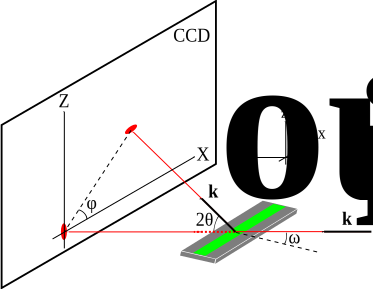
\includegraphics[width=0.8\textwidth]{figures/ripple/analysis/laxs_setup}
  \caption{Experimental reflectivity geometry.}
  \label{fig:laxs_setup}
\end{figure}

%%%%%%%%%%%%%%%%%%%%%%%%%%%%%%%%%%%%%%%%%%%%%%%%%%%%%%%%%%%%%%%%%%%%%%%%%%%%%%%
\newpage
\section{LAXS data reduction}\label{sec:LAXS_data_reduction}
The lattice structure of a stack of bilayers in the ripple is a two dimensional
oblique lattice, and indexing the peaks from an unoriented sample is not 
difficult. In an oriented sample, the stacking $z$ direction and the ripple
$x$ direction are separated, rendering indexing the peaks a trivial task as 
shown in the next subsection.
However, obtaining the form factors from measured intensity is considerably
more involved and requires the development of the three correction factors 
described in the following three subsections.

\subsection{Lattice Structure - Unit Cell}\label{sec:lattice_structure}
The unit cell vectors for the two-dimensional oblique lattice shown in Fig.~\ref{fig:unit_cell}
can be expressed as 
\begin{equation}
  \mathbf{a} = \frac{D}{\tan\gamma}\xhat + D\zhat
\end{equation}
and
\begin{equation}
  \mathbf{b} = \lambda_r\xhat.
\end{equation}
The corresponding reciprocal lattice unit cell vectors are
\begin{equation}
  \mathbf{A} = \frac{2\pi}{D}\zhat
\end{equation}
and
\begin{equation}
  \mathbf{B} = \frac{2\pi}{\lambda_r}\xhat - \frac{2\pi}{\lambda_r\tan\gamma}\zhat.
\end{equation}
The reciprocal lattice vector, $\mathbf{q}_{hk}$ for the Bragg peak with 
Miller indices $(h,k)$ is 
\begin{equation}
  \mathbf{q}_{hk}=h\mathbf{A}+k\mathbf{B},
\end{equation}
so its Cartesian components are
\begin{align}
  & \mathbf{q}_{hk}\cdot\xhat = q_{hk}^x = \frac{2\pi k}{\lambda_r}\\
  & \mathbf{q}_{hk}\cdot\yhat = q_{hk}^y = 0 \\
  & \mathbf{q}_{hk}\cdot\zhat = \qz{hk} = \frac{2\pi h}{D} - \frac{2\pi k}{\lambda_r\tan\gamma}.
\end{align}
Our sample consists of many ripple domains with a uniform distribution of 
in-plane directions of the
ripple wave vector, $\mathbf{b}$ in Fig.~\ref{fig:unit_cell}. 
This means that, for any $(h,k)$ reflection, there is always a domain that has 
an in-plane orientation such that quasi-elastic scattering occurs and a peak 
appears on the CCD.  
In this case, $q_{hk}^x$ and $q_{hk}^y$ may be combined to 
give $q_{hk}^r = 2\pi k/\lambda_r$.  
Fig.~3.2 shows this Miller index pattern from which the in-plane ripple repeat 
distance $\lambda_r$ = 145.0 \AA, the out-of-plane repeat distance 
$D$ = 57.8 \AA, and the oblique angle $\gamma$ = 98.2\textdegree\ for that 
sample were easily obtained.
Values of $q_{hk}^r$ and $\qz{hk}$ for observed reflections are included
in Tables~\ref{tab:obs_intensity1} and \ref{tab:obs_intensity2}.

%%%%%%%%%%%%%%%%%%%%%%%%%%%%%%%%%%%%%%%%%%%%%%%%%%%%%%%%%%%%%%%%%%%%%%%%%%%%%%%
\subsection{Lorentz Correction}\label{sec:Lorentz_correction}
Our sample has in-plane rotational symmetry about the $z$-axis. 
Ignoring mosaic spread to which we will come back later, this means that the sample 
consists of many domains with differing ripple directions, all domains
being parallel to the substrate.  
In sample $q$-space, ripple ($h,k\neq 0$) side peaks are represented as rings 
centered at the meridian, or $q_z$-axis, 
while ($h,k=0$) main peaks are still points on the meridian 
(see Fig.~\ref{fig:ripple_sample_qspace}). 
Then, for an arbitrary incident angle $\omega$, $(h,0)$ peaks are not observed
while side peaks are observed for a range of $\omega$ as will now be explained. 

\begin{figure}[htbp]
  \centering
  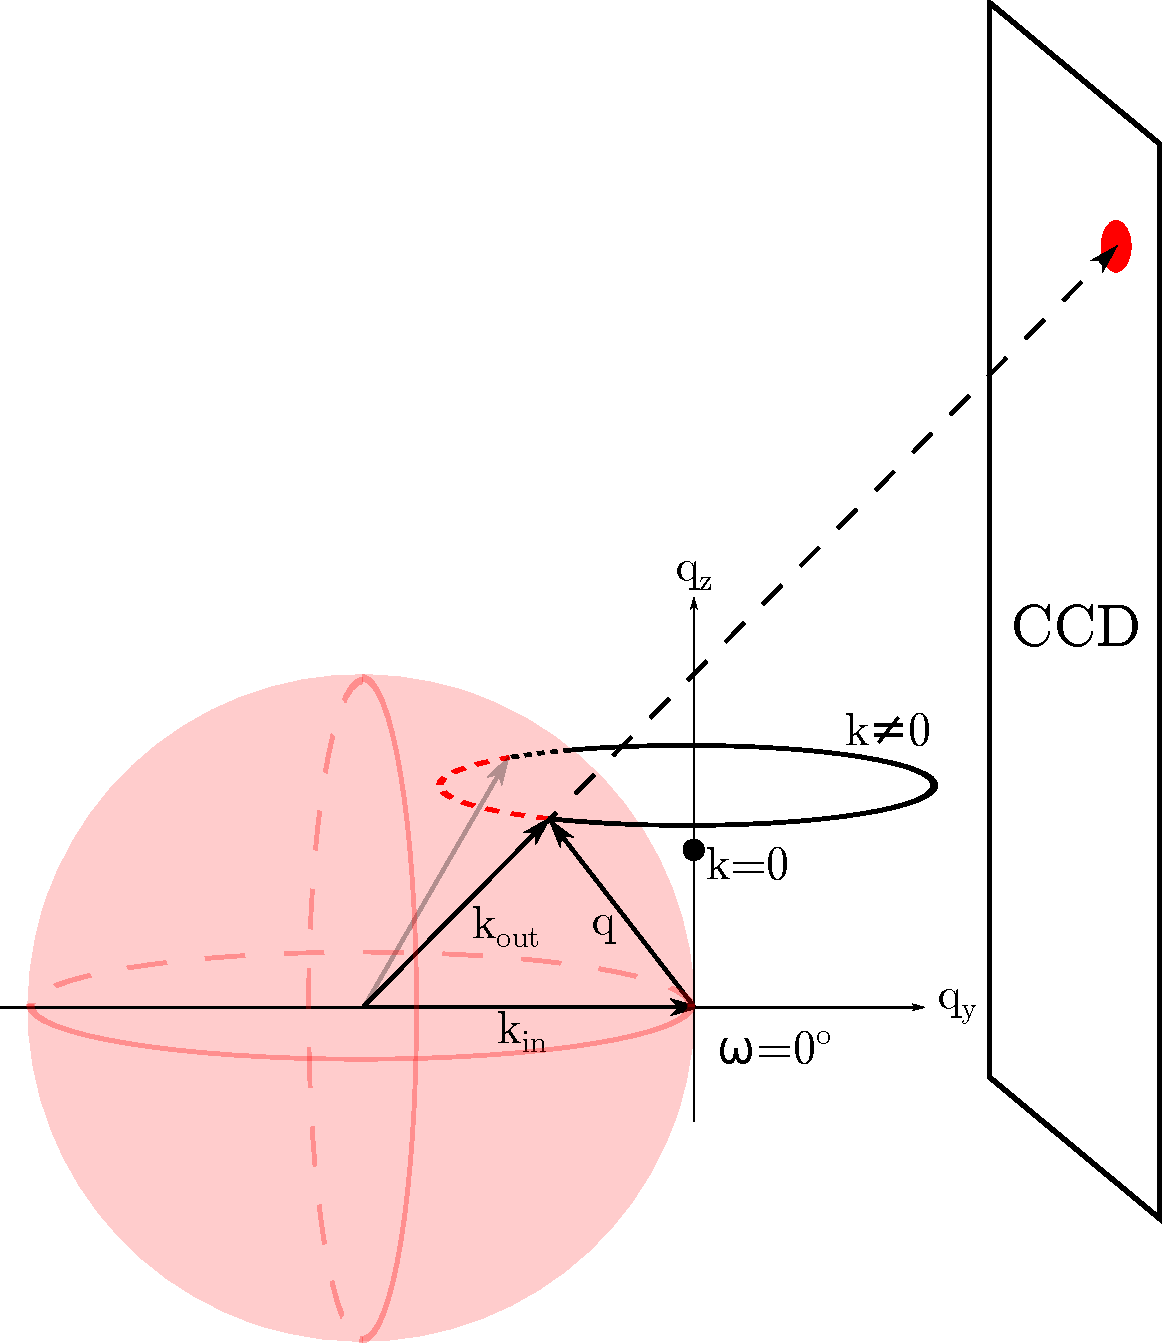
\includegraphics[width=0.8\textwidth]{figures/ripple/analysis/ripple_sample_qspace}
  \caption{Ewald sphere construction to obtain relation between location of 
  scattering peaks on the CCD and their $q$-space values. The incoming X-ray 
  wavevector is $\kin$ and $\kout$ is a scattered X-ray wavevector with 
  $|\kout|=|\kin|$ for the predominant quasi-elastic scattering. 
  The $\mathbf{q}$-space pattern is shown for the ripple phase in the low angle 
  regime. For $(h, k=0)$ Miller indices, there are points labelled $k=0$ on the 
  $q_z$ axis.  
  For $(h,k\neq0)$ there are rings labelled $k\neq0$ centered on the 
  $q_z$-axis. The red dashed line shows the portion of a ring that is inside 
  the Ewald sphere and the portion outside is shown as a black solid line. 
  Diffraction occurs where the ring and the sphere intersect.  For clarity 
  $|\mathbf{q}|$ is drawn large compared to $|\kin|$. For our wavelength
	of 1.175 \AA, $|\kin|=5.35$ \AA$^{-1}$ and for $h=5$,
  $\qz{50}=0.54$ \AA$^{-1}$, one tenth of $|\kin|$.}
  \label{fig:ripple_sample_qspace}
\end{figure}

In order to capture all ($h,k$) peaks in one X-ray exposure, 
the sample was continuously rotated over a range of $\omega$, $\Delta\omega$,
about the $x$-axis. As a result of this rotation, 
the $(h,0)$ main peaks become arcs that subtend an angle $\Delta\omega$,
as shown in Fig.~\ref{fig:ewald_main}, with its length
equal to $\Delta\omega\qz{h0}$. 
The detector records the intersections of these arcs with the 
Ewald sphere, so the intrinsic scattering intensity of the $(h,k=0)$ reflections
is the product of the observed intensity, $\Io{hk}$ with the arc length, that is, 
\begin{equation}
  I_{h0} = \Delta\omega\qz{h0} \Io{h0}. \label{eq:main_ewald}
\end{equation}
This gives the usual Lorentz correction for lamellar orders.

Now, we consider relative intensity of side peaks for a given order $h$.
As described earlier, $(h, k\neq 0)$ side peaks are represented as
rings whose radius is $\qr{hk}$ in the sample $q$-space. 
Because only the domains with the right ripple direction can satisfy the Bragg's condition at a given fixed
angle $\omega$, the intrinsic scattering intensity in this ring is reduced by 
a factor of $2\pi \qr{k}$ compared to the $(h, 0)$ reflections.
This reduction of intensity can be nicely visualized by the Ewald sphere construction
shown in Fig.~\ref{fig:ripple_sample_qspace},
which shows that the entire rings are not intersected by the Ewald sphere at 
a fixed angle. Then, the intrinsic scattering intensity in a ring is
\begin{equation}
  I_{hk\neq 0} \propto 2\pi \qr{hk} \Io{hk}. \label{eq:side_ewald}
\end{equation}
During an X-ray exposure, the sample $q$-space rotates and 
the rings are intersected by the Ewald sphere at all our experimental incident angles $\omega$.
However, as Fig.~\ref{fig:ewald_side} shows, only small parts of the rings
are actually intersected with the Ewald sphere.  
To obtain the full expression for $(h,k\neq 0)$ reflections, we now turn
to a more rigorous calculation.

\begin{figure}[htbp]
  \centering
  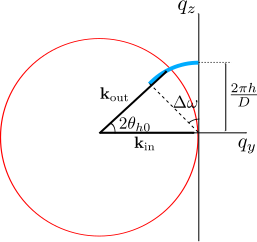
\includegraphics[width=0.45\textwidth]{figures/ripple/analysis/ewald_main}
  \caption{Trajectory of $k=0$ peak as the sample is rotated by $\omega$ is 
  shown as a thick blue line.}
  \label{fig:ewald_main}
\end{figure}

\begin{figure}[htbp]
  \centering
  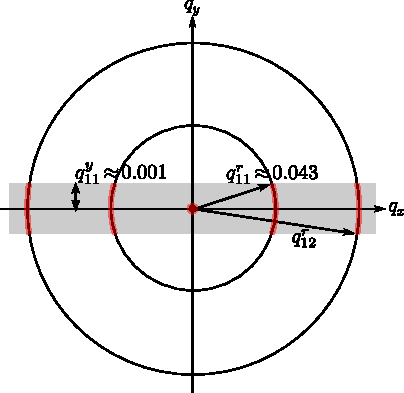
\includegraphics[width=0.45\textwidth]{figures/ripple/analysis/ewald_side_h1_ver1}
  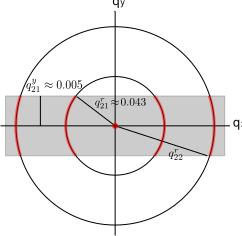
\includegraphics[width=0.45\textwidth]{figures/ripple/analysis/ewald_side_h2_ver1}
  \caption{$q$-space representations of Bragg peaks and Bragg rings 
  for $h$ = 1 and 2 and $k$ = 0, 1, and 2 in $\qz{hk}$ planes.
  The intersection between the Ewald sphere and 
  a Bragg peak/ring is indicated in red. 
  The observed intensity for the $k\neq 0$ orders is proportional to
  the fraction of the length of red arcs in the circumference. This 
  fraction is equal to one for $k=0$ reflections.
  Because the reflections are not in the same $q_z$ plane, the range of $q_y$ 
  integration indicated by the height of the gray rectangle is different for different
  $h$ orders. For $\gamma\neq 90$\textdegree, the range of $q_y$ integration is
  slightly different for different $k$ reflections with the same $h$. 
  The values shown are for $D=58$ \AA, $\lambda_r=145$ \AA, $\gamma=90$\textdegree,
  and $\lambda=1.175$ \AA. For visibility, the height of the gray rectangles 
  is exaggerated by about a facotr of 10 so the magnitude of curvature of arcs 
  is exaggerated.  With the shown curvature, the peaks would have an asymmetric 
  shape in the $q_r$ direction.}
  \label{fig:ewald_side}
\end{figure}

Mathematically, the rotation is  
equivalent to an integration over $\omega$. In low angle X-ray scattering, 
$q_z$ is nearly constant at a given pixel as $\omega$ is varied, 
which can be seen from 
Eq.~(\ref{eq:qxqyqz_small}). As Eq.~(\ref{eq:qxqyqz_small}) shows, 
$\omega$ dependence appears only through $q_y$, 
so rotating the sample is realized by integrating over $q_y$;
formally, we write $d\omega=dq_y/q_z$.
To derive the integration limits on $q_y$, let us consider two cases: 
(1) When $\omega \leq 0$,
the incoming X-ray beam is blocked by the back of the substrate. This sets 
the lower limit of $\omega$ to 0. Plugging $\omega=0$ in Eq.~\ref{eq:qxqyqz_small}),
we find the lower limit of the $q_y$ integration to be $-\lambda q_z^2/(4\pi)$.
(2) When $\omega \geq 2\theta$, the substrate blocks 
the outgoing X-ray, so the maximum $\omega = 2\theta$. 
Within the small angle approximation, $q_z \approx 4\pi\theta/\lambda$. 
Then, the maximum $\omega$ can be expressed as $\lambda q_z/(2\pi)$.
Plugging this expression for $\omega$ in Eq.~(\ref{eq:qxqyqz_small}),
we find the upper limit of the $q_y$ integration to be $\lambda q_z^2/(4\pi)$.
Also integrating over the detector pixels $X$ and $Z$ to obtain integrated intensity, 
we write the observed intensity as
\begin{align}
  \Io{hk} 
    &\propto \int dX \int dZ \int \mathop{d\omega} I_{hk} \nonumber \\
    &\propto \int dq_x \int dq_z 
             \int_{-\frac{\lambda q_z^2}{4\pi}}^{\frac{\lambda q_z^2}{4\pi}} 
             \frac{dq_y}{q_z} 
             I_{hk}(\mathbf{q}),
  \label{eq:I_obs_general}
\end{align}
where $1/q_z$ factor in $q_y$ integration is the usual Lorentz polarization factor
in the small angle approximation. 

For a crystalline sample with in-plane rotational symmetry, the
structure factor of a ripple Bragg peak is  
\begin{equation}
  S_{hk}(\mathbf{q}) = S_{hk}(q_r,q_z) 
  = \frac{1}{2\pi q_r}\delta(q_r-\qr{hk})\delta(q_z-\qz{hk}),
\end{equation} 
where $\qr{hk}=2\pi |k|/\lambda_r$. Thus, the scattering pattern in the 
ripple phase is a 
collection of Bragg rings for $k\neq 0$ centered at the meridian and the 
Bragg peaks for $k=0$ located along the meridian.  
The scattering intensity is $I(\mathbf{q})=|F(\mathbf{q})|^2S(\mathbf{q})$,
where $F(\mathbf{q})$ is the form factor. After the $q_z$ integration,
the observed, integrated intensity of $(h,k)$ peak is proportional to
\begin{equation}
  \Io{hk} 
    \propto \frac{\lvert F_{hk} \rvert^2}{\qz{hk}} \int\mathop{dq_x} 
            \int_{-q_{hk}^{y0}}^{q_{hk}^{y0}}
            \mathop{dq_y} \frac{\delta(q_r-\qr{hk})}{2\pi q_r},
  \label{eq:obs_integration}
\end{equation}
where $q_{hk}^{y0} = \lambda (\qz{hk})^2/(4\pi)$.
For side peaks ($k \neq 0$), we have 
\begin{align}
  \int\mathop{dq_x} \int_{-q_{hk}^{y0}}^{q_{hk}^{y0}}\mathop{dq_y} \frac{\delta(q_r-\qr{hk})}{2\pi q_r}
  &\approx \int_{-q_{hk}^{y0}/\qr{hk}}^{q_{hk}^{y0}/\qr{hk}} \mathop{d\phi} 
          \int \mathop{dq_r} q_r\frac{\delta(q_r-\qr{hk})}{2\pi q_r} \nonumber\\
  &= \frac{q_{hk}^{y0}}{\pi \qr{hk}}. 
  \label{eq:side_integrand}
\end{align}
For main peaks ($k=0$), we have 
\begin{align}
  \int\mathop{dq_x} \int_{-q_{hk}^{y0}}^{q_{hk}^{y0}}\mathop{dq_y} \frac{\delta(q_r-\qr{hk})}{2\pi q_r}
  &= \int_0^{2\pi}\mathop{d\phi} \int\mathop{dq_r} q_r\frac{\delta(q_r-\qr{hk})}{2\pi q_r} \nonumber\\
  &= 1 
  \label{eq:main_integrand}
\end{align}
Using Eq.~(\ref{eq:obs_integration} -- \ref{eq:main_integrand}), 
we write the observed integrated intensity as
\begin{align}
  \Io{h0} &\propto \frac{|F_{h0}|^2}{\qz{h0}} \label{eq:main}\\
  \Io{hk} &\propto \frac{|F_{hk}|^2}{\qz{hk}} \frac{q_{hk}^{y0}}{\pi \qr{hk}}
    = |F_{hk}|^2 \frac{\lambda \qz{hk}}{2\pi}\frac{1}{2\pi \qr{hk}}
    = |F_{hk}|^2 \frac{2\theta_{hk}}{2\pi \qr{hk}}, \label{eq:side}
\end{align}
where $2\theta_{hk} = \lambda \qz{hk}/(2\pi)$ is the incident angle at which 
the outgoing X-ray for the peak $(h,k)$ is blocked by the substrate.
Eq.~(\ref{eq:main}) and (\ref{eq:side}) relate the form factor calculated from
a model to the experimentally observed intensity, and are partially
equivalent to Eq.~(\ref{eq:main_ewald}) and (\ref{eq:side_ewald}). 

%%%%%%%%%%%%%%%%%%%%%%%%%%%%%%%%%%%%%%%%%%%%%%%%%%%%%%%%%%%%%%%%%%%%%%%%%%%%%%%
\subsection{Absorption Correction for LAXS}\label{sec:absorption_correction}
In this section, we derive the absorption correction for an oriented sample. 
The calculation involves an explicit integration over the incident angle, 
$\omega$, which is necessitated by the sample rotation during an X-ray exposure. 
The procedure is to write down an absorption factor, $A(\omega,\theta)$, for a 
given scattering angle 2$\theta$ at a given incident angle $\theta$, and
then integrate over $\omega$. We ignore $q_x$ dependence because the X-ray
path inside the sample is nearly within the $y$-$z$ plane for low angle
scattering. The correction for wide angle scattering is described in a later
section.

\begin{figure}[htbp]
  \centering
  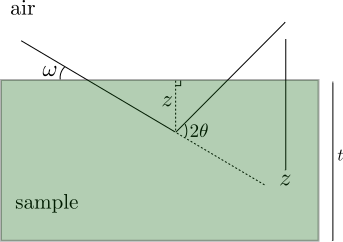
\includegraphics[width=0.5\textwidth]{figures/ripple/analysis/absorption_LAXS}
  \caption{The path of X-rays within the sample. The incident angle is 
  $\omega$ and the total scattering angle is $2\theta$. An X-ray with a
  penetration depth of $z$ is shown. The total thickness of the sample
  is $t$. Refraction correction is negligible for 
  $\theta > 0.5$\textdegree ($h=1$).}
  \label{fig:absorption_LAXS}
\end{figure}

Assume that all the X-rays enter the sample from the top surface. The total scattering
angle is given by $2\theta$ (see Fig.~\ref{fig:absorption_LAXS}).
Let the $z$-axis point downward. At the top surface
(air-sample interface), $z=0$. For X-rays that travel to $z$ and then scatter, the
total path length within the sample is 
\begin{equation}
  L(z,\omega,\theta) 
  = \frac{z}{\sin\omega}+\frac{z}{\sin(2\theta-\omega)} 
  = zg(\omega,\theta),
\end{equation}
where $g(\omega,\theta)=(\sin\omega)^{-1}+\pars{\sin\pars{2\theta-\omega}}^{-1}$.
For each ray, the intensity is attenuated by the sample absorption. 
Compared to the scattering intensity from $z=0$, the attenuated intensity is
\begin{equation}
  I(z,\omega,\theta) = I_0\exp\left(-\frac{L}{\mu}\right),
  \label{eq:ray}
\end{equation}
where $\mu$ is the absorption length of an X-ray. $\mu$ is about 2.6 mm for 
10.5 keV
for both water and lipids in all phases \cite{ref:cxro}.
The observed intensity of scattering from a sample fixed at an angle $\omega$ 
is equal to the integration
of Eq.~(\ref{eq:ray}) over the total thickness of the sample and given by
\begin{align}
  I(\omega,\theta) 
    &= \int_0^t \dz I(z,\omega,\theta)
     = I_0\int_0^t\dz \exp\left(-\frac{g(\omega,\theta)}{\mu}z\right) \nonumber \\
    &= I_0\mu \frac{1-\exp\left(-\frac{t}{\mu}g(\omega,\theta)\right)}{g(\omega,\theta)}.
    \label{eq:I_obs1}
\end{align}
Defining the absorption factor at a fixed angle to be $A(\omega,\theta)$, 
the observed intensity can also be written as
\begin{equation}
  I(\omega,\theta)=A(\omega,\theta)tI_0,
  \label{eq:I_obs2}
\end{equation}
where $tI_0$ is the intensity we would observe for non-absorbed X-rays.
Equating Eq.~(\ref{eq:I_obs1}) and (\ref{eq:I_obs2}), we get
\begin{equation}
  A(\omega,\theta) = \frac{\mu}{t} 
                     \frac{1-\exp\left(-\frac{t}{\mu}g(\omega,\theta)\right)}{g(\omega,\theta)}.
  \label{eq:ang_abs_factor}
\end{equation}
If $\mu$ is taken to infinity (no absorption), $A(\omega,\theta)$ 
goes to 1 as expected.
The absorption factor $A_{h0}$ for the $k=0$ peaks is given by
$A(\omega=\theta=\theta_B)$, plotted in Fig.~\ref{fig:abs_factor}.
As shown, this factor is about 20 \% for $h=1$ peak relative to
$h=4$, so it is not negligible.

\begin{figure}[htbp]
  \centering
  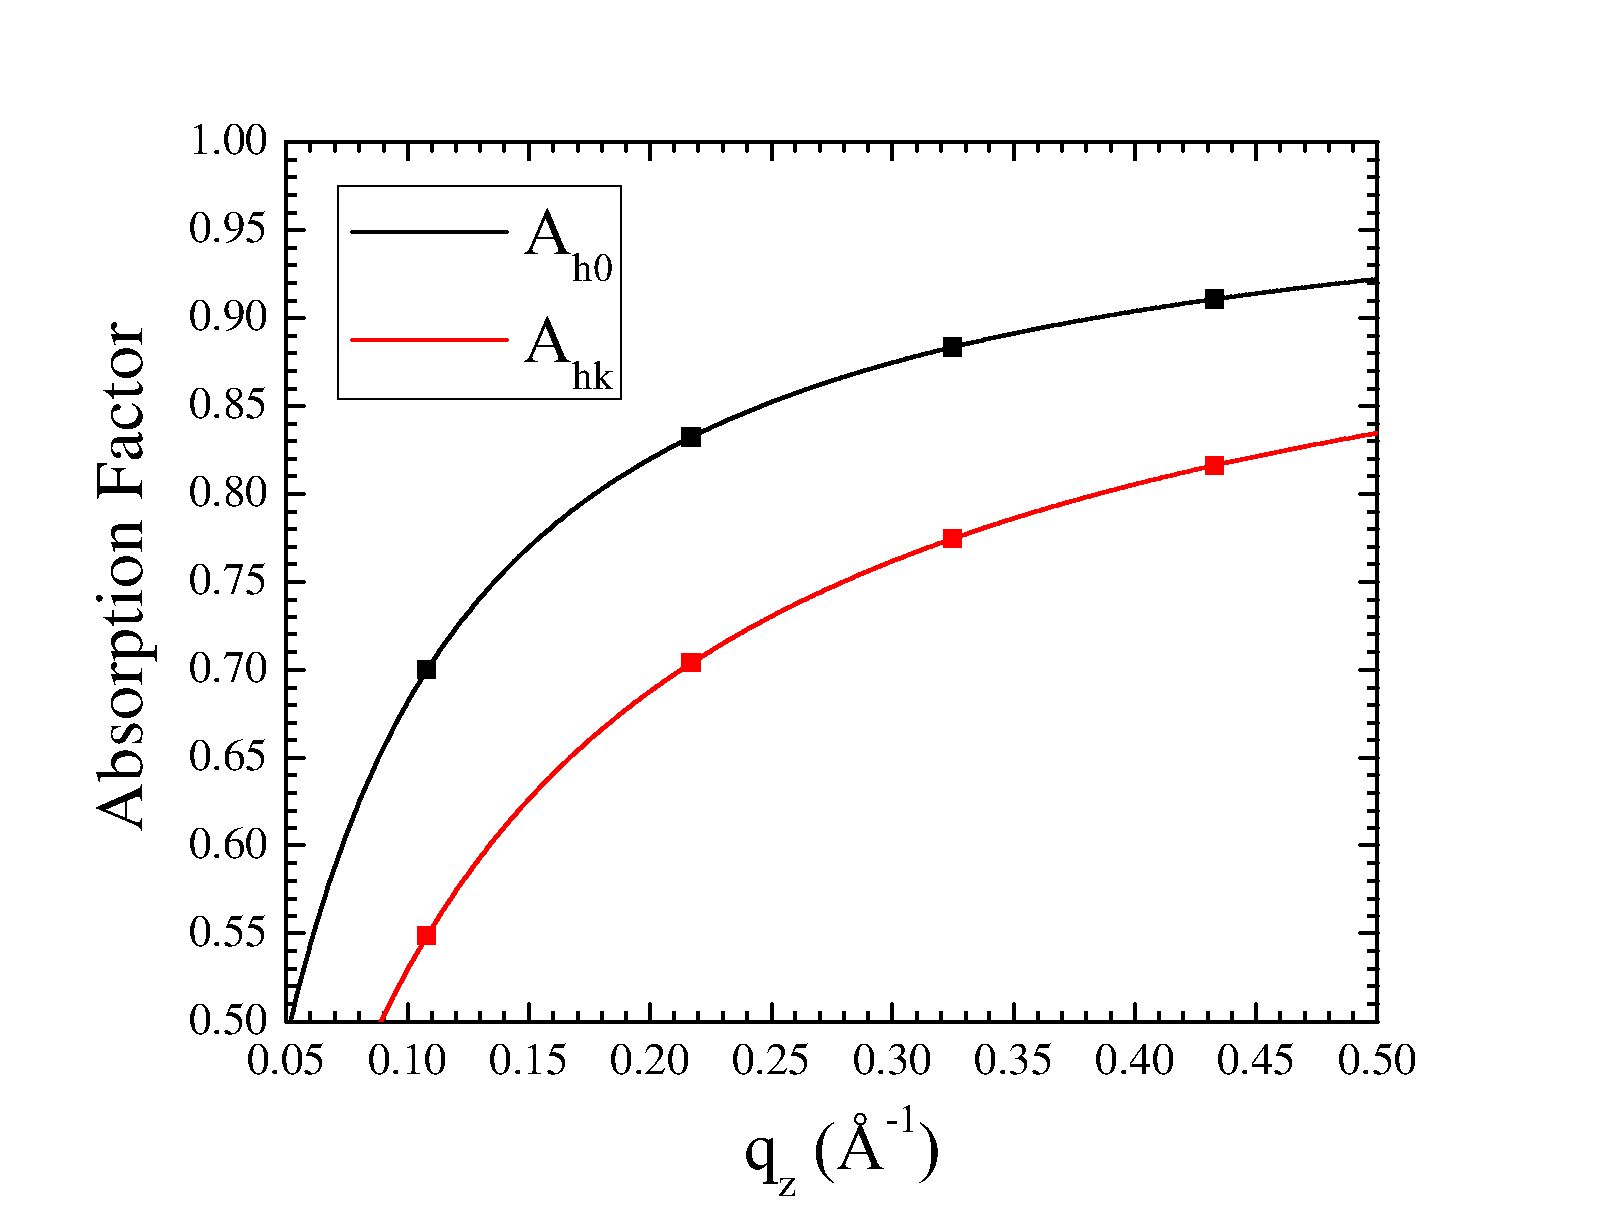
\includegraphics[width=0.7\textwidth]{figures/ripple/analysis/abs_factor}
  \caption{Absorption factors as a function of $q_z \approx 4\pi\theta/\lambda$.
  Values at $q_z=2\pi h/D$ corresponding to $D=57.8$ \AA\ are shown as squares.
  $\mu$ = 2600 $\mu$m, $t$ = 10 $\mu$m, and $\lambda$ = 1.175 \AA.}
  \label{fig:abs_factor}
\end{figure}

\begin{figure}[htbp]
  \centering
  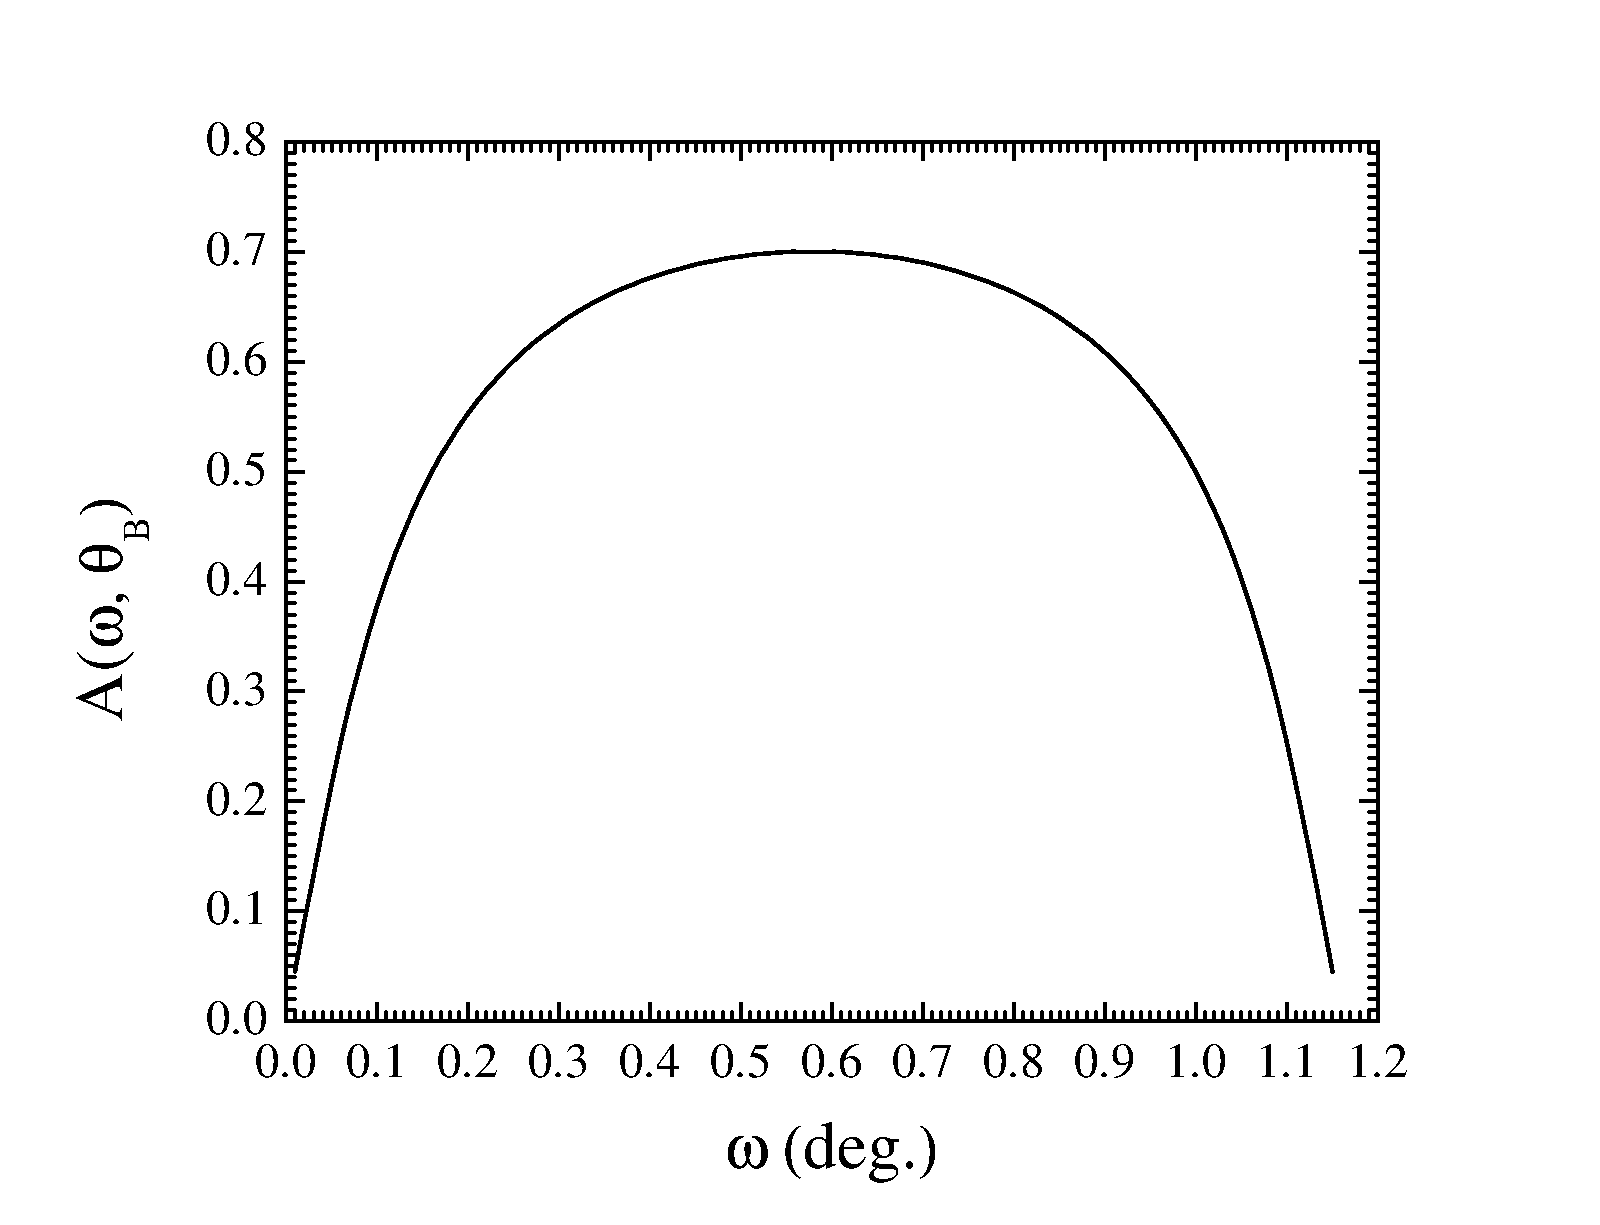
\includegraphics[width=0.7\textwidth]{figures/ripple/analysis/abs_integrand}
  \caption[Eq.~(\ref{eq:ang_abs_factor}) plotted as a function of $\omega$ for 
  $\theta=\theta_B$]{Eq.~(\ref{eq:ang_abs_factor}) plotted as a function of 
  $\omega$ for $\theta=\theta_B=0.58$\textdegree, corresponding to the $h=1$ 
  Bragg
  angle for $D$ = 57.8 \AA.}
  \label{fig:abs_integrand}
\end{figure}

For $k\neq 0$ side peaks, an integration over the incident angle $\omega$
is necessary because these peaks are observable at all our experimental incident angles as
described in section \ref{sec:Lorentz_correction}.
The observed intensity for side peaks from a rotating sample is simply
\begin{equation}
  I_\textrm{obs}(\theta) 
  = \int_0^{2\theta}\textrm{d}\omega I(\omega,\theta).
  \label{eq:total_obs_I}
\end{equation}
The upper integration limit is equal to $2\theta$ because the substrate
completely blocks the scattered X-rays above this angle as discussed in 
section \ref{sec:Lorentz_correction}. Eq.~(\ref{eq:ang_abs_factor}),
which is essentially the integrand in Eq.~(\ref{eq:total_obs_I}), is 
plotted in Fig.~\ref{fig:abs_integrand}. It is maximum when $\omega=\theta$,
meaning that the path length is shortest at the Bragg condition.
The non-attenuated observed intensity is equal to $2\theta t I_0$. We, then, 
define the absorption factor $A(\theta)$ to be the ratio of the total 
observed intensity to the total non-attenuated intensity,
\begin{align}
  A(\theta) \equiv \frac{I_\textrm{obs}(\theta)}{2\theta tI_0}. 
  \label{eq:abs_factor_def}
\end{align}
Using Eq.~(\ref{eq:ang_abs_factor}) and (\ref{eq:total_obs_I})
in (\ref{eq:abs_factor_def}), we arrive
at the final absorption factor
\begin{equation}
  A(\theta) = \frac{1}{2\theta}\int_0^{2\theta}d\omega A(\omega,\theta)
  = \frac{\mu}{2\theta t} \int_0^{2\theta}d\omega 
  \frac{1-\exp\left(-\frac{t}{\mu}g(\omega,\theta)\right)}{g(\omega,\theta)}.
  \label{eq:abs_factor}
\end{equation}
$A_{hk} = A(\theta)$ is plotted in Fig.~\ref{fig:abs_factor}.
The absorption correction $A_c(\theta)$ is the inverse of Eq.~(\ref{eq:abs_factor}). 

%%%%%%%%%%%%%%%%%%%%%%%%%%%%%%%%%%%%%%%%%%%%%%%%%%%%%%%%%%%%%%%%%%%%%%%%%%%%%%%
\subsection{Correction due to mosaic spread}\label{sec:mosaic_spread_correction}
Integrated intensity needs to be corrected for mosaic spread, which consists 
of a distribution of domains of bilayers misoriented with respect to the 
substrate. 
During an X-ray exposure, the sample
was continuously rotated. Due to this rotation, each pixel integrates 
intensity over a range of incident angles $\omega$.
As described in appendix~\ref{app:mosaic_exp}, 
a mosaic spread distribution can be probed
by changing $\omega$, so rotating the sample is essentially  
equivalent to integrating a mosaic spread distribution.
Because the range of the distribution probed is approximately given by $\omega=[0, 2\theta_{hk}]$ 
where $\theta_{hk}$ is the Bragg angle for a $(h,k)$ reflection, 
this range is larger for higher $h$ orders. 
This effect is illustrated in Fig.~\ref{fig:mosaic_contour}.

\begin{figure}[htbp]
  \centering
  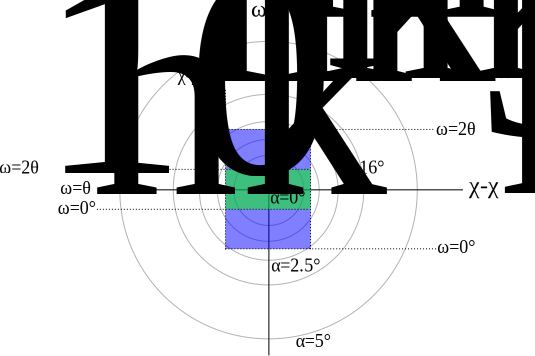
\includegraphics[width=0.9\textwidth]{figures/ripple/analysis/mosaic_contour}
  \caption{Contours of a mosaic spread distribution projected on the $\omega\chi$-plane,
  where $\chi-\chi_{hk}$ is an angle measured from a $(h,k)$ reflection on the detector
  ($\chi=\pi/2-\phi$ in Fig.~\ref{fig:laxs_setup}) and $\theta_{hk}$ is the
  Bragg angle for the $(h,k)$ reflection.
  The distribution function takes a form of Lorentzian centered at $\alpha=0$.
  Domains with $\alpha=0$ are probed at $\omega=\theta_{hk}$ and $\chi=\chi_{hk}$.
  Integrated intensity of $(1,k)$ reflection arises from domains in the green
  shaded area while that of $(3,k)$ reflection is from the
  blue shaded area, which is three times larger.}
  \label{fig:mosaic_contour} 
\end{figure}

We limit 
$\chi-\chi_{hk}$ to go from -1.4\textdegree\ to 1.4\textdegree\
by our choice of integration boxes for the intensity.  
The effect of cutoff on $\chi-\chi_{hk}$ is not very important
because most of observed intensity was included in integration boxes.
In contrast, cutoff on $\omega$ due to substrate blocking the scattering
is important, especially for lower $h$ orders.
 
We take the distribution to be Lorentzian, which has been observed 
experimentally in this laboratory (manuscript in preparation),
\begin{equation}
  P(\alpha) = \frac{N}{\alpha^2+\alpha_M^2},
\end{equation}
where $N$ is a normalization constant and $\alpha_M$ is the HWHM of the 
distribution. $N$ satisfies
\begin{equation}
  N \approx \frac{1}{2\pi}\left(\int_0^{\frac{\pi}{2}}\mathop{d\alpha}
  \frac{\alpha}{\alpha^2+\alpha_M^2}\right)^{-1}.
  \label{eq:mosaic_N}
\end{equation}
We then consider a two dimensional contour map on the $\omega\chi$ plane.
Intensity for a reflection with Bragg angle $\theta_B$ is
given by
\begin{equation}
  I = \int_{-\theta_B}^{\theta_B}\mathop{d\omega} 
  \int_{-\chi_0}^{\chi_0}\mathop{d\chi} P(\alpha)
  = \int_{-\theta_B}^{\theta_B}\mathop{d\omega}
  \int_{-\chi_0}^{\chi_0}\mathop{d\chi}
  \frac{N}{\omega^2+\chi^2+\alpha_M^2}
  \label{eq:mosaic_I}
\end{equation}
After the integration over $\chi$, Eq.~(\ref{eq:mosaic_I}) is
\begin{equation}
  I = 4N\int_0^{\theta_B}\frac{d\omega}{\sqrt{\omega^2+\alpha_M^2}}
  \arctan\pars{\frac{\chi_0}{\sqrt{\omega^2+\alpha_M^2}}}.
  \label{eq:mosaic_I2}
\end{equation}
Eq.~(\ref{eq:mosaic_I2}) is plotted in Fig.~\ref{fig:mosaic_correction}.

\begin{figure}
  \centering
  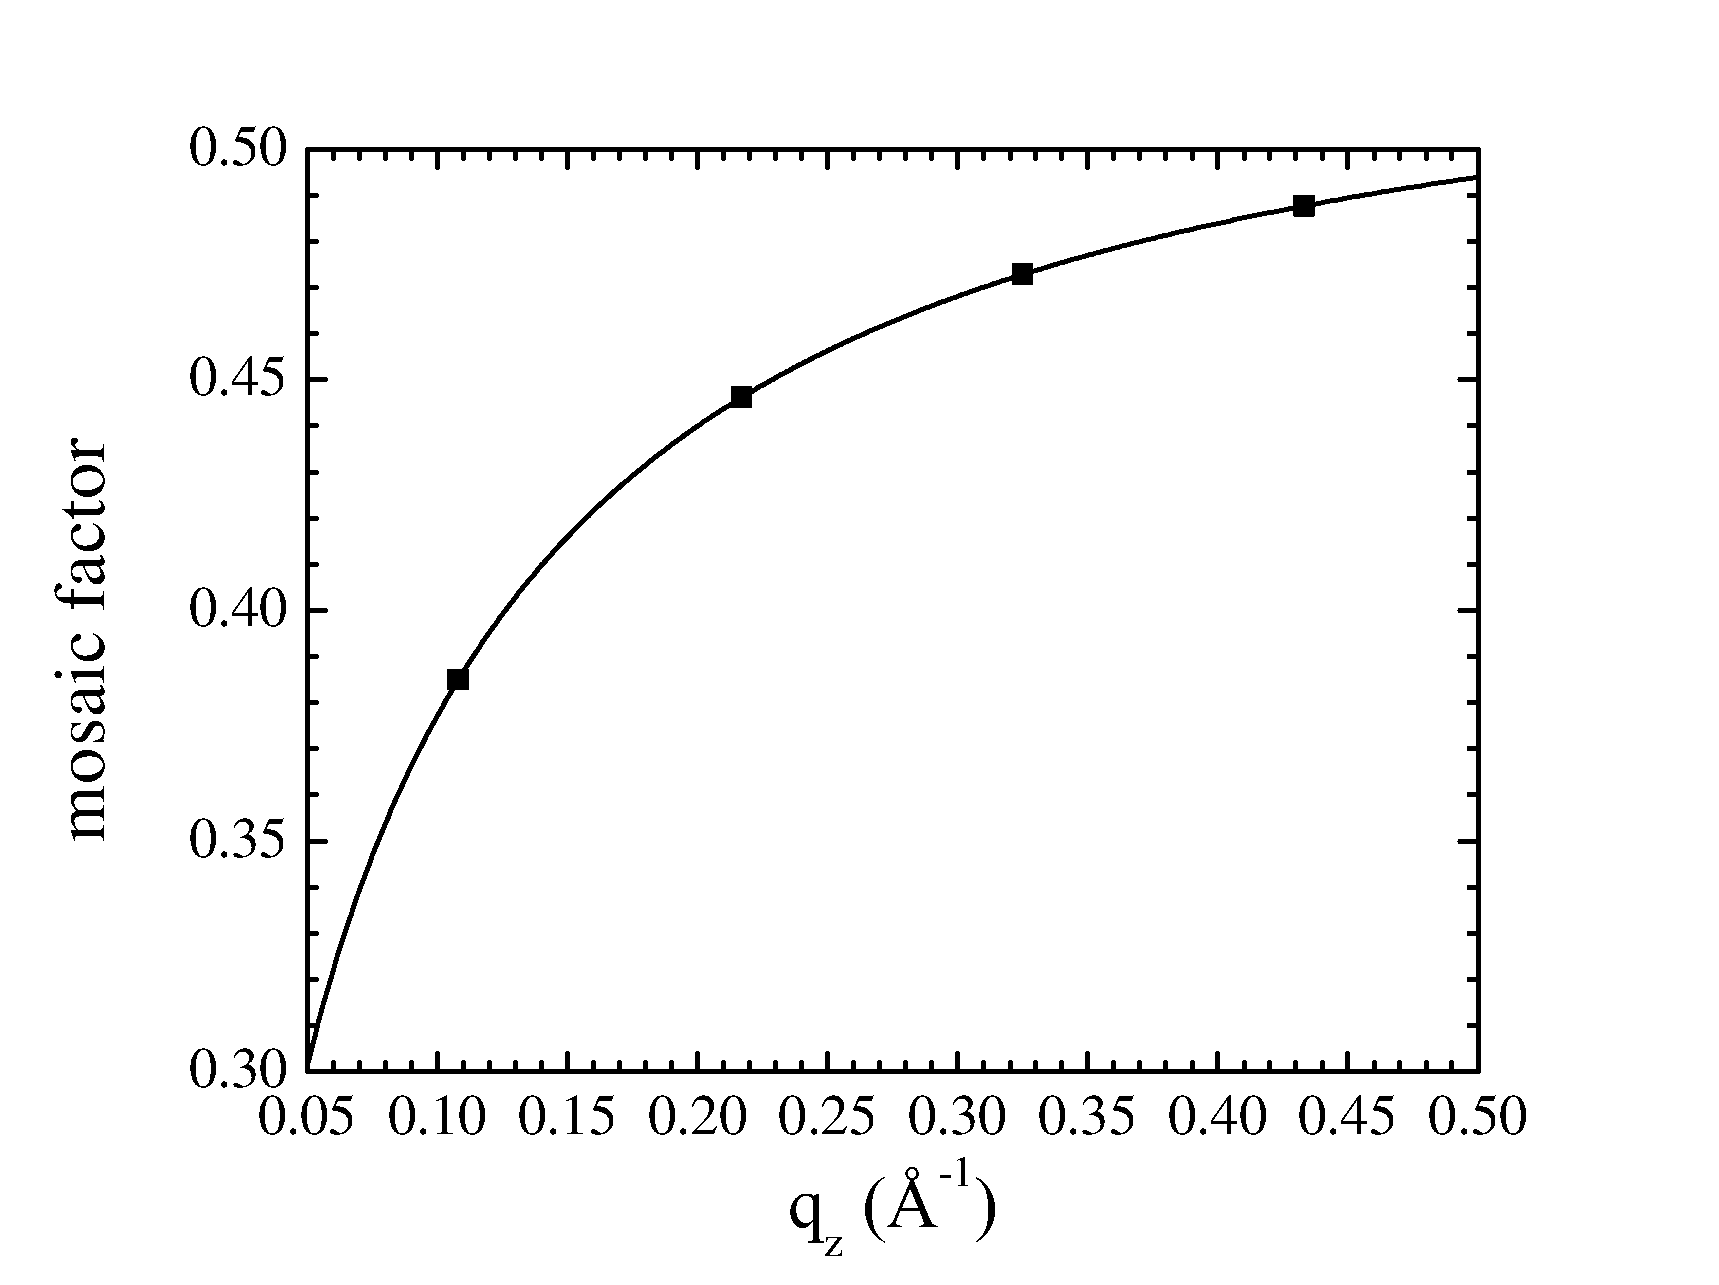
\includegraphics[width=0.7\textwidth]{figures/ripple/analysis/mosaic_correction}
  \caption[Mosaic factor given by Eq.~(\ref{eq:mosaic_I2}) as a function of 
  $q_z\approx 4\pi\theta/\lambda$]{Mosaic factor given by 
  Eq.~(\ref{eq:mosaic_I2}) as a function of 
  $q_z\approx 4\pi\theta/\lambda$. Values at $q_z=2\pi h/D$ corresponding 
  to $D=57.8$ \AA\ are shown as squares. $\alpha_M=0.05$\textdegree\ and 
  $\chi_0$=1.4\textdegree. Eq.~(\ref{eq:mosaic_I2}) reaches $\sim$0.54 at 
  $\theta_B=\pi/2$ and $\chi_0=1.4$\textdegree\ and reaches $\sim$1 at
  $\theta_B=\pi/2$ and $\chi_0=\pi/2$ as expected.}
  \label{fig:mosaic_correction}
\end{figure}

\subsubsection{Synopsis of intensity corrections}
Table~\ref{tab:LAXS_correction1} and \ref{tab:LAXS_correction2} show
the values of the corrections obtained from the analysis in the previous three 
subsections using properties of our samples. The absorption and mosaicity 
corrections are significant for the lowest orders and their product largely 
acounts for the smaller intensities previously noted 
{\jn reference our DHPC paper} for the lower orders of gel phase oriented 
samples compared to unoriented MLV samples which do not have these corrections.  
These two corrections decrease gradually as $h$ increases with small 
modulations with $k$. In contrast, the Lorentz correction varies strongly with 
both $h$ and $k$ although it is the same for the same $h/k$. The importance of 
the previous three sections is emphasized by the result that the largest 
correction for $(1,3)$ is a factor of 367 greater than for the smallest 
correction for $(1,0)$.

\begin{table}[htbp]
  \centering
    \begin{tabular}{rrrrrr}
    \hline
    \multicolumn{1}{c}{$h$} & \multicolumn{1}{c}{$k$} & \multicolumn{1}{c}{Absorption} & \multicolumn{1}{c}{Mosaicity} & \multicolumn{1}{c}{Lorentz} & \multicolumn{1}{c}{All} \\
    \hline    
    1  & -1 & 1.96 & 2.63 & 14.16 & 73.086  \\
    1  & 0  & 1.41 & 2.56 & 0.11  & 0.394   \\
    1  & 1  & 1.79 & 2.56 & 12.67 & 58.027  \\
    1  & 2  & 1.74 & 2.53 & 25.00 & 110.055 \\
    1  & 3  & 1.69 & 2.50 & 34.12 & 144.592 \\
    2  & -2 & 1.45 & 2.27 & 14.19 & 46.738  \\
    2  & -1 & 1.43 & 2.27 & 6.97  & 22.641  \\
    2  & 0  & 1.19 & 2.22 & 0.22  & 0.577   \\
    2  & 1  & 1.41 & 2.22 & 6.45  & 20.187  \\
    2  & 2  & 1.39 & 2.22 & 12.51 & 38.607  \\
    2  & 3  & 1.39 & 2.22 & 18.29 & 56.444  \\
    2  & 4  & 1.39 & 2.22 & 23.92 & 73.827  \\
    2  & 5  & 1.39 & 2.17 & 28.76 & 86.837  \\
    2  & 6  & 1.37 & 2.17 & 33.73 & 100.446 \\
    3  & -2 & 1.30 & 2.13 & 9.31  & 25.723  \\
    3  & -1 & 1.30 & 2.13 & 4.50  & 12.436  \\
    3  & 0  & 1.14 & 2.13 & 0.33  & 0.788   \\
    3  & 1  & 1.28 & 2.08 & 4.35  & 11.586  \\
    3  & 2  & 1.28 & 2.08 & 8.52  & 22.766  \\
    3  & 3  & 1.28 & 2.08 & 12.56 & 33.555  \\
    3  & 4  & 1.27 & 2.08 & 16.42 & 43.295  \\
    3  & 5  & 1.27 & 2.08 & 20.18 & 53.212  \\
    3  & 6  & 1.27 & 2.08 & 23.81 & 62.802  \\
    4  & -3 & 1.23 & 2.04 & 10.54 & 26.557  \\
    4  & -2 & 1.22 & 2.04 & 6.94  & 17.265  \\
    4  & -1 & 1.22 & 2.04 & 3.40  & 8.454   \\
    4  & 0  & 1.10 & 2.04 & 0.44  & 0.976   \\
    4  & 1  & 1.22 & 2.04 & 3.28  & 8.153   \\
    4  & 2  & 1.22 & 2.04 & 6.39  & 15.897  \\
    4  & 3  & 1.21 & 2.04 & 9.50  & 23.450  \\
    4  & 4  & 1.20 & 2.04 & 12.60 & 30.981  \\
    4  & 5  & 1.20 & 2.04 & 15.49 & 38.076  \\
    4  & 6  & 1.20 & 2.04 & 18.35 & 45.126  \\
    \hline
    \end{tabular}%
  \caption{Correction factors for the raw intensities of the ripple LAXS 
  peaks for thickness of an oriented sample $t$ = 10 \AA\ and mosaic
  spread $\alpha_M$ = 0.05\textdegree.}
  \label{tab:LAXS_correction1}%
\end{table}%
    
\begin{table}[htbp]
  \centering
    \begin{tabular}{rrrrrr}
    \hline
    \multicolumn{1}{c}{$h$} & \multicolumn{1}{c}{$k$} & \multicolumn{1}{c}{Absorption} & \multicolumn{1}{c}{Mosaicity} & \multicolumn{1}{c}{Lorentz} & \multicolumn{1}{c}{All}\\
    \hline        
    5  & -3 & 1.19 & 2.00 & 8.44 & 20.084 \\
    5  & -2 & 1.19 & 2.00 & 5.49 & 13.060 \\
    5  & -1 & 1.19 & 2.00 & 2.64 & 6.291  \\
    5  & 0  & 1.08 & 2.00 & 0.54 & 1.169  \\
    5  & 1  & 1.19 & 2.00 & 2.43 & 5.774  \\
    6  & -4 & 1.16 & 2.00 & 9.36 & 21.778 \\
    6  & -3 & 1.16 & 2.00 & 6.92 & 16.094 \\
    6  & -2 & 1.16 & 2.00 & 4.47 & 10.389 \\
    6  & -1 & 1.16 & 2.00 & 2.23 & 5.193  \\
    6  & 0  & 1.06 & 2.00 & 0.65 & 1.389  \\
    6  & 1  & 1.16 & 2.00 & 2.24 & 5.217  \\
    6  & 2  & 1.16 & 2.00 & 4.40 & 10.208 \\
    6  & 3  & 1.15 & 2.00 & 6.38 & 14.657 \\
    6  & 4  & 1.15 & 2.00 & 8.40 & 19.309 \\
    7  & -4 & 1.14 & 1.96 & 7.94 & 17.682 \\
    7  & -3 & 1.14 & 1.96 & 5.86 & 13.060 \\
    7  & -2 & 1.14 & 1.96 & 3.82 & 8.512  \\
    7  & -1 & 1.14 & 1.96 & 1.86 & 4.145  \\
    7  & 0  & 1.05 & 1.96 & 0.76 & 1.569  \\
    8  & 0  & 1.04 & 1.96 & 0.87 & 1.773  \\
    9  & -5 & 1.11 & 1.96 & 7.60 & 16.549 \\
    9  & -4 & 1.11 & 1.96 & 6.07 & 13.233 \\
    9  & -3 & 1.11 & 1.96 & 4.50 & 9.790  \\
    9  & -2 & 1.11 & 1.96 & 2.98 & 6.497  \\
    9  & -1 & 1.11 & 1.96 & 1.50 & 3.263  \\
    9  & 0  & 1.04 & 1.96 & 0.98 & 2.000  \\
    \hline
    \end{tabular}%
  \caption{Corrections for the intensities of the ripple LAXS peaks 
  (continued from Table~\ref{tab:LAXS_correction1})}
  \label{tab:LAXS_correction2}%
\end{table}%

%%%%%%%%%%%%%%%%%%%%%%%%%%%%%%%%%%%%%%%%%%%%%%%%%%%%%%%%%%%%%%%%%%%%%%%%%%%%%%%
\newpage
\section{Results for $|F_{hk}|$ form factors}\label{sec:LAXS_form_factors}

Table~\ref{tab:obs_intensity1} and \ref{tab:obs_intensity2} lists the observed 
$(h,k)$ reflections and their $q_z$ and $q_r$ values for our best sample shown 
in Fig.~\ref{fig:ripple_laxs_images}. The $q_z$ values 
for observed peaks were corrected for index of refraction (Appendix~\ref{app:refraction}).
Column $I^\text{obs}_{hk}$ is the sum of intensity observed within an
integration box centered on the peak with size shown in the box size column.  
These intensities were multiplied by the total correction factor redisplayed 
from Table \ref{tab:LAXS_correction1} and the square root was taken to obtain 
unnormalized  $|F_{hk}|$.  
As there is an arbitrary scale factor in the data, the $|F_{hk}|$ shown in 
Table~\ref{tab:obs_intensity1} were then normalized to set $|F_{10}|$ = 100.

The $\sigma_I$ column in table~\ref{tab:obs_intensity1} gives uncertainties on 
$I^\text{obs}_{hk}$.
The largest contribution to $\sigma_I$ for weak orders was the background 
scattering, which
was assumed to be a constant for each peak and 
estimated by plotting a swath along a given peak 
and seeing where the peak tail ended. This was done visually and repeating 
the process led to differences which determined the estimated $\sigma_I$.  
For some peaks, uncertainty mostly came 
from the mosaic arc of stronger nearby peaks. For example, the (4, -1) peak was a
strong order, but the mosaic arc of its nearby stronger (4, 0) peak  
overlapped with the (4, -1) peak, giving a relatively large uncertainty
on the (4, -1) peak. While most $k<0$ peaks were susceptible to
mosaic arc, $k > 0$ peaks were not. Therefore, though $k> 0$ peaks were weaker
compared to corresponding $k < 0$ peaks, their integrated intensity
had smaller $\sigma_I$. We assigned a large uncertainty on the (3, 1) peak because
it overlapped with the $q_z$ tail of the (3, -1) peak, making separation of 
(3, 1) and (3, -1) difficult. It was also not clear whether the (3, 1) peak
was extinct or not. $\sigma_I$ for this peak was estimated by placing a
box centered at the nominal position of this peak, and it is likely that a fraction
of the intensity assigned to (3, -1) in table~\ref{tab:obs_intensity1} belongs to (3, 1).
The (1, 1) and (1, -1) also overlapped in a similar manner, so their
relative $\sigma_I$ are larger than some of well separated less intense peaks.  
Some peaks, such as (1, 2), (4, 3), (6, 2), (9, -1), (9, -3), and all the 
(8, k) peaks were deemed to be extinct because neighboring peaks had 
observable intensity. As zero is also an observation, these orders were also 
included in the table. 

\begin{table}[htbp]
  \centering
  \begin{tabular}{rrrrcrrrrr}
    \hline
    \multicolumn{1}{c}{$h$} & \multicolumn{1}{c}{$k$} & \multicolumn{1}{c}{$q_z$} & 
    \multicolumn{1}{c}{$q_r$} & \multicolumn{1}{c}{box size} & \multicolumn{1}{c}{$\Io{hk}$} & 
    \multicolumn{1}{c}{$\sigma_I$} & \multicolumn{1}{c}{correction} & \multicolumn{1}{c}{$|F_{hk}|$} &
    \multicolumn{1}{c}{$\sigma_F$} \\
     & & \multicolumn{1}{c}{(\AA$^{-1}$)} & \multicolumn{1}{c}{(\AA$^{-1}$)} & \multicolumn{1}{c}{(pixels)} & ($\times 10^3$) & & & \\ 
    \hline
  1        & -1       & 0.102    & -0.043   & 10 $\times$ 7 & 726.0    & 63.0     & 73.086    & 86.3     & 3.7 \\
  1        & 0        & 0.109    & 0.000    & 10 $\times$ 7 & 180818.0 & 1759.0   & 0.394     & 100.0    & 0.5 \\
  1        & 1        & 0.114    & 0.043    & 10 $\times$ 7 & 228.0    & 28.0     & 58.027    & 43.1     & 2.6 \\
  1        & 2        &          &          &             & 0.0        & 1.0      & 110.055   & 0.0      & 3.9 \\
  1        & 3        & 0.128    & 0.130    & 10 $\times$ 7 & 3.8      & 0.2      & 144.592   & 8.8      & 0.2 \\
  2        & -2       & 0.206    & -0.087   & 10 $\times$ 7 & 49.2     & 3.5      & 46.738    & 18.0     & 0.6 \\
  2        & -1       & 0.212    & -0.044   & 10 $\times$ 7 & 1818.0   & 20.0     & 22.641    & 76.0     & 0.4 \\
  2        & 0        & 0.218    & 0.000    & 10 $\times$ 7 & 10200.0  & 174.0    & 0.577     & 28.7     & 0.2 \\
  2        & 1        & 0.224    & 0.043    & 10 $\times$ 7 & 550.0    & 10.0     & 20.187    & 39.5     & 0.4 \\
  2        & 2        & 0.231    & 0.086    & 10 $\times$ 7 & 112.0    & 3.0      & 38.607    & 24.6     & 0.3 \\
  2        & 3        & 0.237    & 0.129    & 10 $\times$ 7 & 27.0     & 0.2      & 56.444    & 14.6     & 0.1 \\
  2        & 4        & 0.243    & 0.173    & 10 $\times$ 7 & 8.2      & 0.4      & 73.827    & 9.2      & 0.2 \\
  2        & 5        & 0.250    & 0.214    & 10 $\times$ 7 & 2.6      & 0.7      & 86.837    & 5.6      & 0.7 \\
  2        & 6        & 0.256    & 0.257    & 10 $\times$ 7 & 1.2      & 0.2      & 100.446   & 4.1      & 0.3 \\
  3        & -2       & 0.314    & -0.087   & 15 $\times$ 7 & 305.0    & 15.0     & 25.723    & 33.2     & 0.8 \\
  3        & -1       & 0.321    & -0.043   & 15 $\times$ 7 & 1205.0   & 22.0     & 12.436    & 45.9     & 0.4 \\
  3        & 0        & 0.326    & 0.000    & 15 $\times$ 7 & 1566.0   & 110.0    & 0.788     & 13.2     & 0.5 \\
  3        & 1        &          &          & 15 $\times$ 7 & 0.0      & 31.0     & 11.586    & 0.0      & 7.1 \\
  3        & 2        & 0.339    & 0.086    & 15 $\times$ 7 & 32.4     & 1.6      & 22.766    & 10.2     & 0.2 \\
  3        & 3        & 0.345    & 0.129    & 15 $\times$ 7 & 39.1     & 0.9      & 33.555    & 13.6     & 0.2 \\
  3        & 4        & 0.352    & 0.172    & 15 $\times$ 7 & 27.7     & 0.7      & 43.295    & 13.0     & 0.2 \\
  3        & 5        & 0.358    & 0.215    & 15 $\times$ 7 & 12.2     & 0.3      & 53.212    & 9.6      & 0.1 \\
  3        & 6        & 0.364    & 0.258    & 15 $\times$ 7 & 3.5      & 0.5      & 62.802    & 5.6      & 0.4 \\
  4        & -3       & 0.417    & -0.131   & 20 $\times$ 8 & 142.0    & 8.0      & 26.557    & 23.0     & 0.6 \\
  4        & -2       & 0.423    & -0.087   & 20 $\times$ 8 & 755.4    & 19.0     & 17.265    & 42.8     & 0.5 \\
  4        & -1       & 0.429    & -0.043   & 20 $\times$ 8 & 429.6    & 34.0     & 8.454     & 22.6     & 0.9 \\
  4        & 0        & 0.435    & 0.000    & 20 $\times$ 8 & 1917.0   & 23.0     & 0.976     & 16.2     & 0.1 \\
  4        & 1        & 0.441    & 0.043    & 20 $\times$ 8 & 45.3     & 7.2      & 8.153     & 7.2      & 0.6 \\
  4        & 2        & 0.448    & 0.085    & 20 $\times$ 8 & 43.6     & 2.4      & 15.897    & 9.9      & 0.3 \\
  4        & 3        &          &          & 20 $\times$ 8 & 0.0      & 1.3      & 23.450    & 0.0      & 2.1 \\
  4        & 4        & 0.461    & 0.173    & 20 $\times$ 8 & 2.1      & 0.4      & 30.981    & 3.0      & 0.3 \\
  4        & 5        & 0.467    & 0.215    & 20 $\times$ 8 & 3.2      & 0.3      & 38.076    & 4.1      & 0.2 \\
  4        & 6        & 0.473    & 0.259    & 20 $\times$ 8 & 1.0      & 1.1      & 45.126    & 2.5      & 1.1 \\
    \hline
  \end{tabular}
  \caption{Observed intensity for $h$ = 1 to 4 at $D=57.8$, $\lambda_r=145$, and 
  $\gamma=98.2$\textdegree.}
  \label{tab:obs_intensity1}
\end{table}  

\begin{table}[htbp]
  \centering
  \begin{tabular}{rrrrcrrrrr}
    \hline
    \multicolumn{1}{c}{$h$} & \multicolumn{1}{c}{$k$} & \multicolumn{1}{c}{$q_z$} & 
    \multicolumn{1}{c}{$q_r$} & \multicolumn{1}{c}{box size} & \multicolumn{1}{c}{$\Io{hk}$} & 
    \multicolumn{1}{c}{$\sigma_I$} & \multicolumn{1}{c}{correction} & \multicolumn{1}{c}{$|F_{hk}|$} &
    \multicolumn{1}{c}{$\sigma_F$} \\
     & & \multicolumn{1}{c}{(\AA$^{-1}$)} & \multicolumn{1}{c}{(\AA$^{-1}$)} & \multicolumn{1}{c}{(pixels)} & & & & \\ 
    \hline
  5        & -3       & 0.525    & -0.132   & 25 $\times$ 9  & 86.2     & 6.8      & 20.084    & 15.6     & 0.6 \\
  5        & -2       & 0.532    & -0.087   & 25 $\times$ 9  & 145.0    & 4.0      & 13.060    & 16.3     & 0.2 \\
  5        & -1       & 0.538    & -0.042   & 25 $\times$ 9  & 63.4     & 3.4      & 6.291     & 7.5      & 0.2 \\
  5        & 0        & 0.544    & 0.000    & 25 $\times$ 9  & 260.0    & 4.0      & 1.169     & 6.5      & 0.1 \\
  5        & 1        & 0.550    & 0.040    & 25 $\times$ 9  & 50.0     & 2.8      & 5.774     & 6.4      & 0.2 \\
  6        & -4       & 0.628    & -0.175   & 30 $\times$ 10 & 11.4     & 0.8      & 21.778    & 5.9      & 0.2 \\
  6        & -3       & 0.635    & -0.131   & 30 $\times$ 10 & 15.6     & 0.9      & 16.094    & 5.9      & 0.2 \\
  6        & -2       & 0.641    & -0.085   & 30 $\times$ 10 & 10.1     & 1.8      & 10.389    & 3.8      & 0.3 \\
  6        & -1       & 0.647    & 0.043    & 30 $\times$ 10 & 16.3     & 3.0      & 5.193     & 3.4      & 0.3 \\
  6        & 0        & 0.653    & 0.000    & 30 $\times$ 10 & 60.2     & 4.7      & 1.389     & 3.4      & 0.1 \\
  6        & 1        & 0.659    & 0.044    & 30 $\times$ 10 & 20.4     & 1.5      & 5.217     & 3.9      & 0.1 \\
  6        & 2        &          &          & 30 $\times$ 10 & 0.0      & 0.6      & 10.208    & 0.0      & 0.9 \\
  6        & 3        & 0.672    & 0.128    & 30 $\times$ 10 & 5.9      & 0.3      & 14.657    & 3.5      & 0.1 \\
  6        & 4        & 0.679    & 0.170    & 30 $\times$ 10 & 4.2      & 0.3      & 19.309    & 3.4      & 0.1 \\
  7        & -4       & 0.737    & -0.174   & 35 $\times$ 10 & 40.0     & 1.1      & 17.682    & 10.0     & 0.1 \\
  7        & -3       & 0.743    & -0.130   & 35 $\times$ 10 & 36.0     & 1.8      & 13.060    & 8.1      & 0.2 \\
  7        & -2       & 0.749    & -0.085   & 35 $\times$ 10 & 15.0     & 7.3      & 8.512     & 4.2      & 0.9 \\
  7        & -1       & 0.755    & -0.042   & 35 $\times$ 10 & 22.0     & 2.3      & 4.145     & 3.6      & 0.2 \\
  7        & 0        & 0.760    & 0.000    & 35 $\times$ 10 & 36.0     & 1.8      & 1.569     & 2.8      & 0.1 \\
  8        & 0        &          &          &                & 0.0      & 3.0      & 1.773     & 0.0      & 0.9 \\
  9        & -5       & 0.951    & -0.215   & 35 $\times$ 10 & 16.0     & 3.0      & 16.549    & 6.1      & 0.5 \\
  9        & -4       & 0.957    & -0.173   & 35 $\times$ 10 & 16.9     & 3.0      & 13.233    & 5.6      & 0.5 \\
  9        & -3       &          &          & 35 $\times$ 10 & 0.0      & 8.0      & 9.790     & 0.0      & 3.3 \\
  9        & -2       & 0.969    & -0.086   & 35 $\times$ 10 & 10.0     & 2.9      & 6.497     & 3.0      & 0.4 \\
  9        & -1       &          &          & 35 $\times$ 10 & 0.0      & 6.0      & 3.263     & 0.0      & 1.7 \\
  9        & 0        & 0.981    & 0.000    & 35 $\times$ 10 & 17.0     & 10.0     & 2.000     & 2.2      & 0.6 \\
    \hline
  \end{tabular}
  \caption{Observed intensity for $h$ = 5 to 9 at $D=57.8$, $\lambda_r=145$, and 
  $\gamma=98.2$\textdegree\ (continued from Table~\ref{tab:obs_intensity1}).}
  \label{tab:obs_intensity2}
\end{table}

To assign uncertainties to the absolute 
form factors $|F|=\sqrt{I}$ requires propagating $\sigma_I$ to $\sigma_F$.
To do this, we estimated the most likely upper bound on each measured intensity 
$I+\sigma_I$. The most likely upper bound for $|F|$ was determined by
$(|F|+\sigma_F)^2=I+\sigma_I$, which gives $\sigma_F$,
\begin{equation}
\label{eq:simga_F}
  \sigma_F=|F|(-1+\sqrt{1+\frac{\sigma_I}{|F|^2}}).
\end{equation}
In the small $\sigma_I/I$ regime, $\sigma_F=\sigma_I/(2|F|)$. In the 
large $\sigma_I/I$ regime, $\sigma_F=\sqrt{\sigma_I}$. For the lower limit,
a similar consideration gives the same uncertainty $\sigma_F=\sigma_I/(2|F|)$
for the small $\sigma_I/I$. The lower limit in the $\sigma_I/I$ regime
should be zero for the absolute form factors $|F|$. For the form factor $F$,
we take $\sigma_F$ given by Eq.~(\ref{eq:simga_F}) as an estimated 
uncertainty. For very weak peaks whose intensity could not be determined but
whose nearby peaks were observed, we assigned $|F|$ = 0 and 
$\sigma_F = \sqrt{\sigma_I}$ where $\sigma_I$ was estimated based on the
background scattering intensity at the $q$ value corresponding to those
unobserved weak peaks. 

Our best oriented sample in Fig.~3.2 had almost the same $D$, $\gamma$, and 
only slightly different ${\lambda}_r$ as the best data of of Wack and Webb 
\cite{ref:Wack89} from an unoriented sample. 
Table~\ref{tab:cmu_vs_wack} compares our oriented 
$\left|F_{hk}^\text{ori}\right|$ with the unoriented 
$\left|F_{hk}^\text{un}\right|$. The most obvious comparison is that there 
are very few unoriented orders, only 18 compared to 60 orders in tables 
\ref{tab:obs_intensity1} and \ref{tab:obs_intensity2}. 
{\jn We have to discuss and maybe include the (0,k) orders.}  
The $k=5$ and $k=6$ reflections shown in Table~\ref{tab:cmu_vs_wack} provides 
higher in-plane resolution in the oriented data and the observability of the 
lamellar orders all the way to $h=9$ provides three times higher resolution 
across the bilayer.

As discussed extensively in the previous section, oriented samples require 
complex corrections, so 
comparison with the relatively straigthforward Lorentz correction from an 
unoriented sample with similar structure allows us to check our corrections.  
Although the ratios of the normalized form factors vary from 0.62 to 1.38, 
there appears to be no sign that our corrections are flawed.  We propose a 
different reason why the ratios deviate so much from unity. In X-ray data from 
an oriented sample, most peaks were
well separated on the two-dimensional CCD, so integrating a peak intensity was 
usually straightforward.
In contrast, intensities from unoriented data are collapsed onto 
one-dimensional and overlap much more, making separation of intensity 
difficult.  Three such pairs of overlapping peaks are highlighted in 
Table~\ref{tab:cmu_vs_wack}.  
We show a modified $\left|F_{hk}^\text{un}\right|$ in 
Table~\ref{tab:cmu_vs_wack} where we have shifted some intensity from 
the (1, 0) peak to the (1, -1) peak and some intensity from the (2, 0) peak 
to the (2, -1) peak.  
Although there is a remaining discrepancy for the (1, 1) reflection, 
the modified ratios are generally improved. Of course, even though it makes 
sense to compare these unoriented and oriented samples, one should not expect 
perfect agreement, especially as the ripple wavelength differes by 2.3\%.  

\begin{table}[htbp]
  \centering
  \begin{tabular}{rrrrrrrr}
    \hline
    \multicolumn{1}{c}{$h$} & \multicolumn{1}{c}{$k$} & \multicolumn{1}{c}{$q$} & \multicolumn{1}{c}{unoriented} & \multicolumn{1}{c}{oriented} & \multicolumn{1}{c}{ratio} & \multicolumn{1}{c}{modified} & \multicolumn{1}{c}{ratio} \\
     & & \multicolumn{1}{c}{(\AA$^{-1}$)} & \multicolumn{1}{c}{$|F_{hk}^{un}|$} & \multicolumn{1}{c}{$|F_{hk}^{ori}|$} &  & $\left|F_{hk}^{un}\right|$ & \\
    \hline
    1 & -1 & {\color{red}0.111}   & 60.8  & 86.3  & 0.70 & 83.0  & 0.96 \\
    1 &  0 & {\color{red}0.108}   & 100.0 & 100.0 & 1.00 & 100.0 & 1.00 \\
    1 &  1 & 0.123                & 26.9  & 43.1  & 0.62 & 29.9  & 0.69 \\
    1 &  2 &                      &       & 0.0   &      &       &      \\
    1 &	 3 & 0.185                & 7.6   & 8.8   & 0.87 & 8.4   & 0.96 \\
    2 &	-2 & 0.224                & 15.1  & 18.0  & 0.84 & 16.8  & 0.93 \\
    2 &	-1 & {\color{blue}0.215}  & 71.2  & 76.0  & 0.94 & 85.1  & 1.12 \\
    2 &  0 & {\color{blue}0.217}  & 39.7  & 28.7  & 1.38 & 30.9  & 1.08 \\
    2 &	 1 & 0.228                & 33.9  & 39.5  & 0.86 & 37.6  & 0.95 \\
    2 &  2 & 0.246                & 22.7  & 24.6  & 0.92 & 25.2  & 1.02 \\
    2 &	 3 & 0.271                & 14.2  & 14.6  & 0.97 & 15.8  & 1.08 \\
    2 &  4 & 0.301                & 7.8   & 9.2   & 0.85 & 8.7   & 0.94 \\
    2 &  5 & 0.329                &       & 5.6   &      &       &      \\
    2 &  6 &                      &       & 4.1   &      &       &      \\
	  3 &	-2 & {\color{green}0.325} & 29.3  & 33.2  & 0.88 & 32.5  & 0.98 \\
    3 & -1 & 0.322                & 44.2  & 45.9  & 0.96 & 49.1  & 1.07 \\
    3 &  0 & {\color{green}0.325} & 12.0  & 13.2  & 0.91 & 13.3  & 1.01 \\
    3 &  1 &                      &       & 0.0   &      &       &      \\
    3 &  2 & 0.350                & 10.5  & 10.2  & 1.03 & 11.7  & 1.15 \\
    3 &  3 & 0.370                & 14.9  & 13.6  & 1.10 & 16.5  & 1.22 \\
    3 &  4 & 0.394                & 10.0  & 13.0  & 0.77 & 11.1  & 0.86 \\
    3 &  5 &                      &       & 9.6   &                     \\
    3 &  6 &                      &       & 5.6   &                     \\
    \hline
  \end{tabular}
  \caption{Comparison of form factors $\left|F_{hk}^\text{un}\right|$ for the 
  unoriented sample from Wack and Webb \cite{ref:Wack89} and 
  $\left|F_{hk}^\text{ori}\right|$ from an oriented sample from this study. 
  The ratio $\left|F_{hk}^\text{un}\right|/\left|F_{hk}^\text{ori}\right|$ of 
  unoriented to oriented form factors is shown.  Three pairs of reflections 
  with very nearly the same $q$ values are shown in color.  A modification is 
  shown that partitions the total intensity of unoriented reflections with 
  nearly the same $q$, as described in the text.}
  \label{tab:cmu_vs_wack}
\end{table}

%%%%%%%%%%%%%%%%%%%%%%%%%%%%%%%%%%%%%%%%%%%%%%%%%%%%%%%%%%%%%%%%%%%%%%%%%%%%%%%%
\newpage
\section{Models to fit the $|F_{hk}|$ and obtain the phases}\label{sec:LAXS_models}
In order to obtain electron density profiles, one requires the phase factors 
for the $|F_{hk}|$.  
Once the phases are obtained, an experimental relative electron density map 
$\rho(\mathbf{r})$ is obtained
by using
\begin{equation}
  \rho(x,z) = \sum_{h,k} \Phi_{hk} \left|F_{hk}^\text{exp}\right| \cos(q_{hk}^xx+q_{hk}^zz),
  \label{eq:Fourier_reconstruction}
\end{equation}
where $\Phi_{hk}$ is the phase factor.  
Fortunately, the ripple phase has a center of inversion symmetry, so 
$\Phi_{hk}$ is limited to be either $+1$ or $-1$. Nevertheless, that still 
leaves $2^{60}$ possibilities for our oriented data.  
It was shown by Sun \textit{et al.} \cite{ref:Sun96} that devising plausible 
models with structural parameters, such as those indicated in Fig. 3.1, and 
fitting those models to the observed $|F_{hk}|$ gave a robust set of phase 
factors for the low resolution data of Wack and Webb \cite{ref:Wack89}.  
That strategy will be followed here.

Following Ref.~\cite{ref:Sun96} the electron density model for $\rho(x,z)$ within 
the unit cell is described
as the convolution of a ripple contour function $C(x,z)$ and the transbilayer
electron density profile $T_\psi(x,z)$,
\begin{equation}
  \rho(x,z) = C(x,z) * T_\psi(x,z).
\end{equation}
The form factor $F(\mathbf{q})$ is the Fourier transform of the electron density.
By the convolution theorem, 
\begin{equation}
  F(\mathbf{q}) = F_C(\mathbf{q})F_T(\mathbf{q}),
\end{equation}
where $F_C(\mathbf{q})$ and $F_T(\mathbf{q})$ are the Fourier transform 
of $C(x,z)$ and $T_\psi(x,z)$, respectively.
We employed standard nonlinear least squares fitting procedures using
the Levenberg-Marquardt algorithm.
The software for data fitting was written in Python using 
the lmfit package \cite{ref:lmfit}.

%%%%%%%%%%%%%%%%%%%%%%%%%%%%%%%%%%%%%%%%%%%%%%%%%%%%%%%%%%%%%%%%%%%%%%%%%%%%%%%%
\subsection{Contour Part of the Form Factor}\label{sec:contour}
As in Ref.\cite{ref:Sun96}, we take the ripple profile to have a sawtooth profile. Its
amplitude is $A$ and the projection of the major arm on the 
ripple direction is $\xM$ as shown in Fig.~\ref{fig:unit_cell}. 
Then, we write the ripple profile as
\begin{equation}
  u(x) = \left\{
    \begin{array}{ccc}
    -\frac{A}{\lambda_r-x_0}\left(x+\frac{\lambda_r}{2}\right) 
      & \text{for} 
      & -\frac{\lambda_r}{2} \leq x < -\frac{x_0}{2}, \\
    \frac{A}{x_0}x 
      & \text{for} 
      & -\frac{x_0}{2} \leq x \leq \frac{x_0}{2}, \\
    -\frac{A}{\lambda_r-x_0} \left(x-\frac{\lambda_r}{2}\right)
      & \text{for} 
      & \frac{x_0}{2} < x \leq \frac{\lambda_r}{2}.
    \end{array} \right.
  \label{eq:sawtooth}
\end{equation}
The ripple profile has inversion symmetry, so that the resulting
form factor is real. $A$ and $\xM$ are fitting parameters that depend 
on the integrated intensity of each peak while $D$, $\lambda_r$, and $\gamma$
are determined from measuring the positions of the Bragg peaks.

In order to allow the electron density along the ripple direction to 
modulate, we include two additional parameters, one to allow for the electron
density across the minor side to be different by a ratio $f_1$ from the 
electron density across the major side and a second parameter $f_2$, which
is multiplied by $\delta$ functions $\delta(x \pm \xM/2)$ to allow for 
a different electron density near the kink between the major and the minor
sides. The full expression for the contour part of the form factor $\FC(\mathbf{q})$,
which is a two dimensional Fourier transform of Eq.~\ref{eq:sawtooth},
is found in Appendix~\ref{app:FC}.

%%%%%%%%%%%%%%%%%%%%%%%%%%%%%%%%%%%%%%%%%%%%%%%%%%%%%%%%%%%%%%%%%%%%%%%%%%%%%%%%
\subsection{Transbilayer Part of the Form Factor}\label{sec:transbilayer}
The hybrid model developed by Wiener \textit{et al.} \cite{ref:Wiener89} has
been successful in modeling the electron density profile in the gel phase.
The hybrid model with two Gaussian functions each representing the headgroup and
terminal methyl group was employed by Sun \text{et al.} \cite{ref:Sun96}
for phasing the ripple phase X-ray data published by Wack and Webb \cite{ref:Wack89}.
We employed the same model for fitting our data 
since it was shown to be very successful in fitting the ripple X-ray data.
Because our data contain more data points at larger $q$, we also used
a model that has three  Gaussian functions, two of which represent the headgroup 
and the other one represents the terminal methyl group. 

In the hybrid model, the terminal methyl region of the bilayer is represented
as a Gaussian function \cite{ref:Wiener89}. The headgroups are represented by one 
and two Gaussian
functions in 1G and 2G hybrid model, respectively. The methylene and water 
regions are each treated as a constant. The gap between the two constants is 
represented by a sine function. Then, for half of the bilayer, 
$0 \leq z \leq D/2$, the electron density has the form, 
\begin{equation}
  \rho(z) = \rhog(z) + \rhos(z) + \rhob(z),
\end{equation}
where the Gaussian part is given by 
\begin{equation}
  \rhog(z) = \sum_{i=1}^{1\text{ or }2} \rhoh{i}
             e^{-(z-\zh{i})^2/(2\sigmah{i}^2)} + \rhom e^{-z^2/(2\sigmam^2)},
\end{equation}
the strip part is given by
\begin{equation}
  \rhos(z) = \left\{
    \begin{array}{ccc}
      \rhochtwo & \text{for } & 0 \leq z < \zchtwo, \\
      \rhow   & \text{for } & \zw \leq z \leq D/2,
    \end{array}
  \right.
\end{equation}
and the bridging part is given by
\begin{equation}
  \rhob(z) = \frac{\rhow-\rhochtwo}{2} \cos \bracks{
    \frac{-\pi}{\deltazh}(z-\zw)} + \frac{\rhow+\rhochtwo}{2} \\
  \text{\quad for \quad} \zchtwo < z < \zw.
\end{equation}
with $\deltazh=\zw-\zchtwo$. Here, we assume $\zh{2}>\zh{1}$. 
Table \ref{tab:zchtwozw} shows the definitions of $\zchtwo$ and $\zw$.

\begin{table}[htbp]
  \centering
  \begin{tabular}{c c c}
    \hline
     & 1G & 2G \\
    \hline
    $\zchtwo$ & $\zh{1}-\sigmah{1}$ & $\zh{1}-\sigmah{1}$ \\
    $\zw$ & $\zh{1}+\sigmah{1}$ & $\zh{2}+\sigmah{2}$ \\
    \hline  
  \end{tabular}
  \caption{Definitions of $\zchtwo$ and $\zw$}
  \label{tab:zchtwozw}
\end{table}

The transbilayer profile along $x=-z\tan\psi$ can be obtained by rotating
the coordinates $x$ and $z$ by $\psi$ in the clockwise direction and
reexpressing $\rho(z)$ in terms of the rotated coordinates. This leads
to replacing $x$ with $x'=x\cos\psi+z\sin\psi$ and
$z$ with $z'=-x\sin\psi+z\cos\psi$. Then, the rotated transbilayer profile is
\begin{equation}
  \rho(x,z) = \delta(x+z\tan\psi)\bracks{\rhog(z') + \rhos(z') + \rhob(z')}.
  \label{eq:rotated_profile}
\end{equation}

Taking the two dimensional Fourier transform of Eq.~(\ref{eq:rotated_profile})
leads to the transbilayer part of the form factor,
\begin{align}
  F_\mathrm{T} 
  &= \int_{-\frac{D}{2}}^{\frac{D}{2}} \int_{-\frac{\lambda_r}{2}}^{\frac{\lambda_r}{2}} 
     \bracks{\rho(x,z)-\rhow} e^{i(q_xx+q_zz)} dxdz \\
  &= F_\mathrm{G} + F_\mathrm{S} + F_\mathrm{B}.
\end{align}
The form factor is calculated in the minus fluid convention, 
where the bilayer electron density
is measured with respect to the electron density of the surrounding solvent.
The expression for $F_\mathrm{T}$ is rather messy, so 
the derivation and full expression are in Appendix~\ref{app:FT}. Here, 
we note that
the fitting parameters in this model are $\zh{i}$, $\sigmah{i}$, and 
$\rhoh{i}$ for each of the two headgroup Gaussian functions, $\sigmam$ and
$\rhom$ for
the terminal methyl Gaussian, $\psi$ for
the lipid tilt, and an overall scaling factor. $\rhochtwo$ is absorbed into 
the overall scaling factor. The contour part of the 
form factor has four more parameters ($A$, $\xM$, $f_1$, and $f_2$).
In total, the modified 2G hybrid model implements 13 structural parameters.
Initially, we made $\zh{i}$, $\psi$, $A$, $\xM$, $f_1$, and $f_2$ free 
parameters
to guide the nonlinear least square procedure to find a reasonable fit
while the other parameters were fixed to the corresponding gel phase values 
reported in Ref.~\cite{ref:Wiener89}. 
The best estimate of the gel phase structure was reported in
Ref.~\cite{Tristram-Nagle02}. Precise values for the fixed parameters
were not important because we then freed those parameters to find the best fit
once a reasonable initial fit was obtained.  

%%%%%%%%%%%%%%%%%%%%%%%%%%%%%%%%%%%%%%%%%%%%%%%%%%%%%%%%%%%%%%%%%%%%%%%%%%%%%%%%
\subsection{Some results of model fitting}\label{sec:LAXS_model_results}
Table~\ref{tab:LAXS_models} summarizes representative fits obtained by a nonlinear
least square fitting procedure. Fit1 and Fit2 were fits using the 1G hybrid model,
and Fit3--Fit7 were with the 2G hybrid model. As Table~\ref{tab:LAXS_models} shows, 
Fit5 produced the smallest $\chi^2$ value. This fit was arrived by 
starting with
Fit3, then freeing the widths of the three Gaussian (Fit4), 
and finally freeing the amplitudes of the Gaussian.
We also tried a different route; from Fit3, we freed up the amplitudes of 
the Gaussian (Fit6) and then set the widths of the Gaussian free, arriving  
at Fit7. 
We consistently obtained model
form factors that were too small compared to the experimental ones 
for ($h$, $k$) = (3, 0), (6, $k$), and (9, 0). This can be understood by
inspecting the contour part of the form factor $F_C(\mathbf{q})$ 
given by Eq.~\ref{eq:FC}.
The model form factor $F(\mathbf{q})$ is a product of
$F_C(\mathbf{q})$ and $F_T(\mathbf{q})$.
Figure~\ref{fig:FC} plots a two dimensional map of $|F_C(\mathbf{q})|$ for
$\lambda_r$ = 145 \AA, $A$ = 21.5 \AA, $\xM$ = 103 \AA, $f_1=0.5$,
and $f_2=-3$, values of which are taken from Fit5.
It shows that $|F_C(\mathbf{q})|$ takes very small values at 
($h, k$) = (3, 0), (6, 0)--(6,4), and (9, 0), leading to small values of
the model $F(\mathbf{q})$ for those peaks as well. These weak spots in $|\FC(\mathbf{q})|$
can be moved by varying $A$ and $\xM$. However, $A$ and $\xM$ are very 
sensitive to strong peaks that are on the white streak in Fig.~\ref{fig:FC}:
namely, ($h, k$) = (1, 0), (1, -1), (2, 0), (2, -1), (3, -1), (3, -2), and so on.
Then, for our data set, minima in the $\chi^2$ space are normally found
with values of $A$ and $\xM$ that result in $\FC(\mathbf{q})$ similar to the 
one shown in Fig.~\ref{fig:FC}.
This analysis 
suggests that better fis to those underestimated orders may require a different model
for the contour part of the form factor rather than trying various
models for the transbilayer part of the form factor $\FT(\mathbf{q})$. 
Since the sawtooth profile is a very reasonable assumption, an improvement
should be made in modeling the kink regions.
For example, introducing a short plateau parallel to the ripple $x$-axis
instead of the sharp turn in the kink region of the current model would
lead to a band of intensity along the $q_z$ axis, which could bring about 
larger values of $|\FC(\mathbf{q})|$ at those underestimated peak positions.
We did not consider improving our models because we were only interested in the predicted
phases for calculating an electron density profile.

\begin{table}[htbp]
  \centering
  \begin{tabular}{cccccccc}
    \hline
          & Fit1 & Fit2 & Fit3 & Fit4 & Fit5 & Fit6 & Fit7 \\
    model & M1G  & M1G  & M2G  & M2G  & M2G  & M2G  & M2G  \\   
    \hline
    $\chi^2$ & 11996 & 9664  & 19458 & 8827  & 8525  & 8905  & 8883 \\
    $A$     & 20.4  & 24.2  & 22.1  & 21.5  & 21.5  & 21.4  & 21.5 \\
    $x_M$   & 98.5  & 118.8 & 92.6  & 104.0 & 102.9 & 102.1 & 102.7 \\
    $f_1$    & 0.489 & 0.726 & 0.776 & 0.515 & 0.538 & 0.516 & 0.511 \\
    $f_2$    & 0*    & -11.3 & -6.06 & -2.77 & -2.81 & -2.62 & -2.63 \\
    $\psi$   & 15.2\textdegree & 14.3\textdegree & 10.5\textdegree & 14.4\textdegree & 14.4\textdegree & 15.1\textdegree & 14.8\textdegree \\
    $\zh{1}$  & 19.8  & 19.7  & 18.1  & 19.5  & 18.7  & 19.1  & 19.0 \\
    $\sigmah{1}$ & 3.43* & 3.43* & 2.94* & 3.06  & 2.51  & 2.94* & 2.97 \\
    $\rhoh{1}$ & 10.77* & 10.77* & 9.91* & 9.91* & 7.03  & 8.38  & 8.45 \\
    $\zh{2}$  & NA    & NA    & 20.0  & 20.4  & 22.4  & 23.2  & 23.0 \\
    $\sigmah{2}$ & NA    & NA    & 1.47* & 3.17  & 1.38  & 1.47* & 1.72 \\
    $\rhoh{2}$ & NA    & NA    & 7.27* & 7.27* & 3.75  & 2.83  & 3.00 \\
    $\sigmam$ & 1.67* & 1.67* & 1.83* & 2.47  & 2.53  & 1.83* & 1.87 \\
    $\rhom$ & 9.23* & 9.23* & 10.9* & 10.9* & 5.15  & 6.87  & 6.97 \\
    \hline
  \end{tabular}
  \caption{Model parameters. Fit1 and Fit2 were performed with the M1G model while 
  Fit3 to 7 were with the M2G model. \\ *Parameters were fixed to the values shown.}
  \label{tab:LAXS_models}
\end{table}

\begin{figure}[htbp]
  \centering
  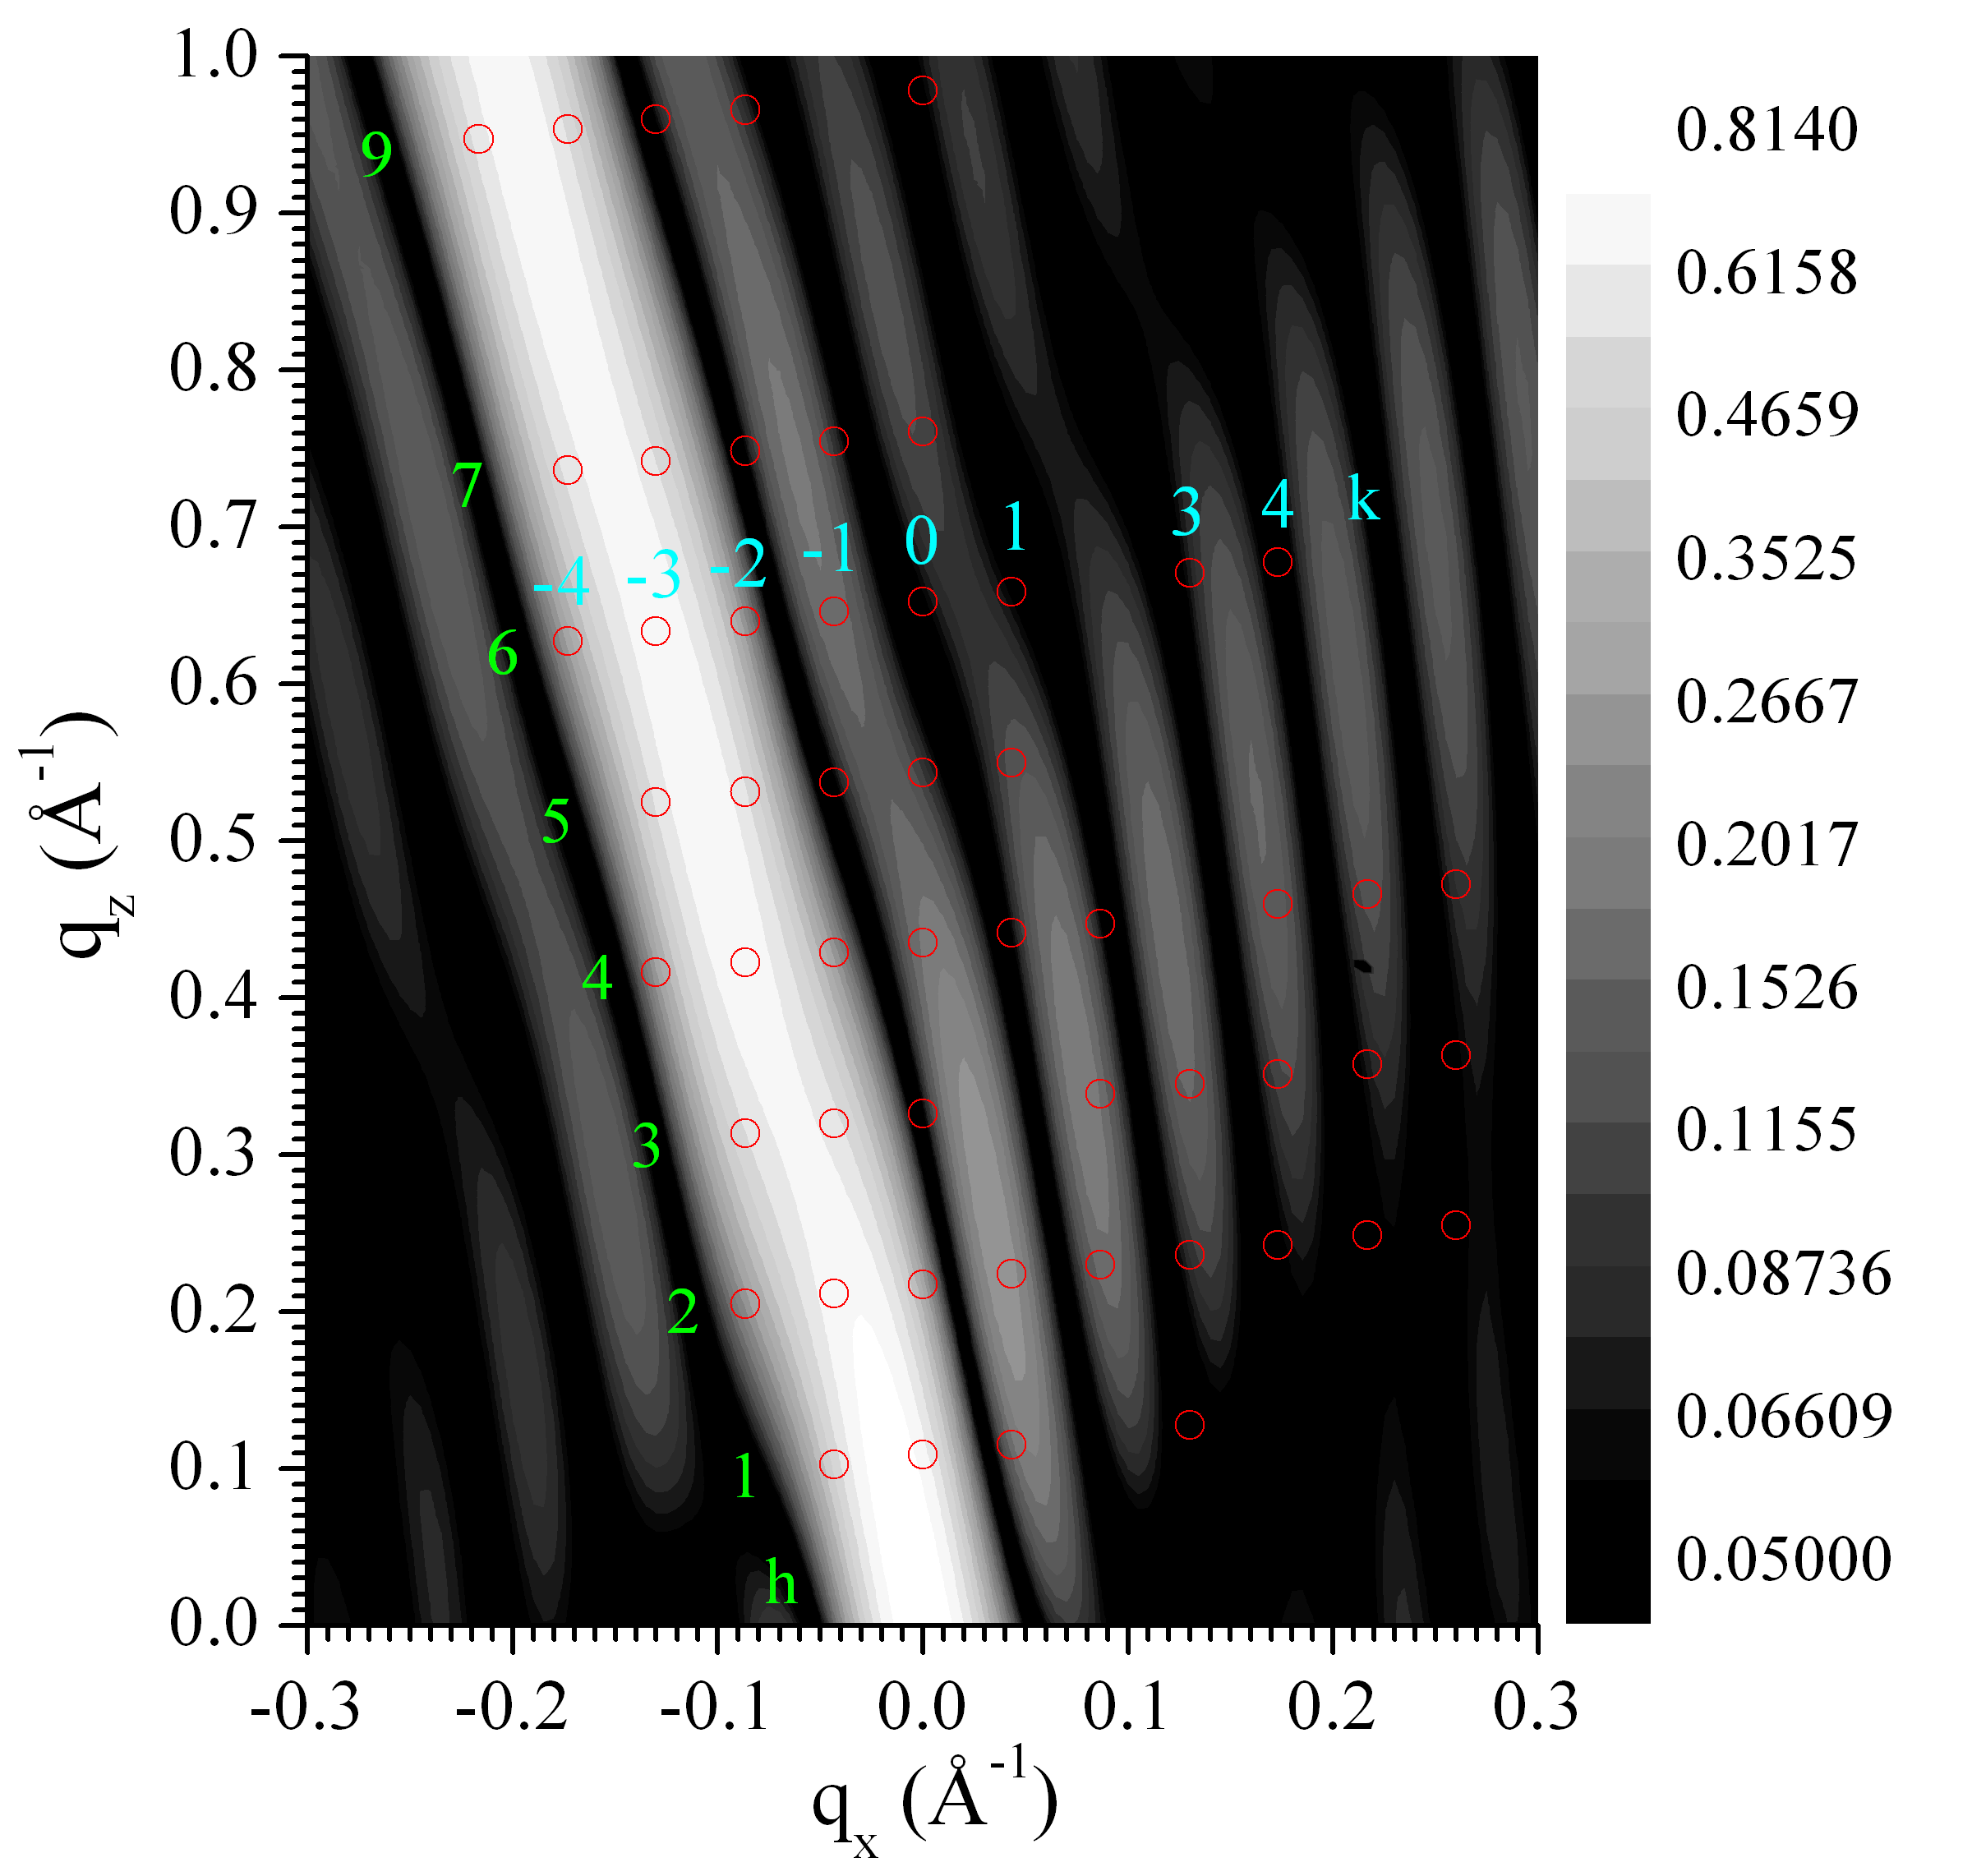
\includegraphics[width=0.9\textwidth]{figures/ripple/model/FT}
  \caption[Two dimensional map of $\FC$]
  {Two dimensional map of the contour part of the form factor $|\FC(\mathbf{q})|$ given by
  Eq.~\ref{eq:FC}. The color is in a log scale shown by the color bar.
  Red circles are the positions of the observed peaks. The actual
  experimental data (Fig.~\ref{fig:ripple_laxs_images}) had left-right symmetry 
  because of in-plane powder of the sample.
  $h$ and $k$ indices are labeled for some of the peaks in green and cyan,
  respectively. The experimentally observed form factors are given by 
  the product $|\FC(\mathbf{q})||\FT(\mathbf{q})|$.}
  \label{fig:FC}
\end{figure}

\subsection{Results for the phase factors}\label{sec:LAXS_phases_results}
It is important to emphasize that the goal of model fitting is to obtain the 
best phase factors, not to obtain the best physical values for these 
structural parameters.  The best values of those parameters will be obtained 
in the next section~\ref{sec:LAXS_edp} by combining the phase factors we 
determine in this subsection with the experimental $|F_{hk}|$.  
Tables \ref{tab:LAXS_fits1} and \ref{tab:LAXS_fits2} show the phases that 
were determined by the various fits described in the previous subsection and 
listed in Table \ref{tab:LAXS_models}. The column labeled `consensus phase'
shows that the phase factor was the same for all the models for most of the 
reflections for which $\pm$ is entered.  Reflections with an asterisk in the 
consensus column are extinct, so any consensus phase factor is irrelevant for 
the electron density profile in Eq.~(\ref{eq:Fourier_reconstruction}). 
We flag phase factors with a question 
mark as being undetermined by models.  In the case of the (1, 3) reflection, 
there is a near consensus that $\Phi_{13}=+1$, but the model values of 
$|F_{13}|$ are considerably smaller than the experimental value, suggesting 
that $\Phi_{13}$ might have either sign.  We have also flagged $\Phi_{7,-2}$ 
for this reason even though all models give $+1$. The most serious lack of 
consensus is for the (6, $k$) reflections where the best models Fit5 and Fit7 
give opposite signs. For the $(6,-3)$ reflection, both models give values of 
$|F_{6,-3}|$ similar in size to the experimental value which is well 
determined to be non-zero, but these two models give opposite $\Phi_{6,-3}$ 
phase factors.  This emphasizes that, while the phase problem has been 
considerably reduced from $2^{60}$, it is still necessary to consider several 
phase combinations to extract the best structural parameters.
\begin{table}[htbp]
  \centering
\begin{tabular}{rrrrrrrrrcrr}
%   & $\chi^2$ & 11996 & 9664 & 19458 & 8827 & 8525 & 8905 & 8883 & \multicolumn{1}{l}{} & \multicolumn{1}{l}{} \\   
\hline
& & \multicolumn{7}{c}{Model $F_{hk}$} & consensus & \multicolumn{1}{c}{Data} & \multicolumn{1}{c}{error} \\
\cline{3-9}
\multicolumn{1}{c}{$h$} & \multicolumn{1}{c}{$k$} & \multicolumn{1}{c}{Fit1} & \multicolumn{1}{c}{Fit2} & \multicolumn{1}{c}{Fit3} & \multicolumn{1}{c}{Fit4} & \multicolumn{1}{c}{Fit5} & \multicolumn{1}{c}{Fit6} & \multicolumn{1}{c}{Fit7} & phase & \multicolumn{1}{c}{$\left|F_{hk}\right|$} & \multicolumn{1}{c}{$\sigma_F$} \\ 
\hline
1 & -1 & -74.0 & -71.6 & -39.4 & -78.4 &  -77.1 & -79.1 &  -79.8 & - &  86.3 & 3.7 \\ 
1 &  0 & -94.3 & -89.2 & -63.1 & -98.6 & -100.0 & -99.6 & -100.1 & - & 100.0 & 0.5 \\ 
1 &  1 &  23.7 &  19.9 &  19.9 &  23.9 &   25.2 &  24.1 &   24.2 & + &  43.1 & 2.6 \\ 
1 &  2 &  -6.0 &  -2.3 &  -8.3 &  -6.0 &   -6.9 &  -5.9 &   -6.0 & * &   0.0 & 3.9 \\ 
1 &  3 &   0.3 &  -3.7 &   6.9 &   1.4 &    2.0 &   1.5 &    1.4 & ? &   8.8 & 0.2 \\ 
2 & -2 & -17.2 & -20.2 & -28.5 & -19.7 &  -20.4 & -20.1 &  -20.1 & - &  18.0 & 0.6 \\ 
2 & -1 & -62.2 & -59.1 & -53.9 & -67.9 &  -66.5 & -65.7 &  -66.9 & - &  76.0 & 0.4 \\ 
2 &  0 & -32.1 & -31.9 & -30.8 & -33.2 &  -33.0 & -33.0 &  -33.1 & - &  28.7 & 0.2 \\ 
2 &  1 &  31.8 &  30.2 &  32.3 &  31.5 &   31.5 &  32.1 &   32.0 & + &  39.5 & 0.4 \\ 
2 &  2 & -25.0 & -24.2 & -22.9 & -24.0 &  -23.9 & -24.3 &  -24.3 & - &  24.6 & 0.3 \\ 
2 &  3 &  15.0 &  15.0 &  14.8 &  14.9 &   14.9 &  14.9 &   14.9 & + & 14.6 & 0.1 \\ 
2 &  4 &  -6.1 &  -5.2 & -12.0 &  -8.6 &   -8.9 &  -8.6 &   -8.5 & - & 9.2 & 0.2 \\ 
2 &  5 &   1.1 &  -2.4 &  10.2 &   6.6 &    7.0 &   6.8 &    6.6 & + & 5.6 & 0.7 \\ 
2 &  6 &   0.1 &   5.5 &  -4.0 &  -7.2 &   -7.1 &  -7.0 &   -7.0 & - & 4.1 & 0.3 \\ 
3 & -2 &  34.2 &  33.3 &  29.9 &  40.3 &   40.6 &  39.9 &   40.1 & + & 33.2 & 0.8 \\ 
3 & -1 &  39.4 &  39.1 &  27.6 &  45.5 &   44.9 &  44.0 &   44.4 & + & 45.9 & 0.4 \\ 
3 &  0 &  -3.2 &  -4.3 &  -2.3 &  -4.3 &   -4.0 &  -4.1 &   -4.2 & - & 13.2 & 0.5 \\ 
3 &  1 &  -9.4 &  -6.9 & -11.2 &  -9.2 &   -9.6 &  -9.8 &   -9.5 & * & 0.0 & 7.1 \\ 
3 &  2 &  14.1 &  12.4 &  15.0 &  14.0 &   14.3 &  14.5 &   14.3 & + & 10.2 & 0.2 \\ 
3 &  3 & -12.9 & -13.7 & -12.5 & -13.1 &  -13.1 & -13.2 &  -13.1 & - & 13.6 & 0.2 \\ 
3 &  4 &   8.6 &  11.7 &   9.0 &   9.5 &    9.4 &   9.2 &    9.3 & + & 13.0 & 0.2 \\ 
3 &  5 &  -4.1 &  -7.9 &  -7.1 &  -6.0 &   -5.9 &  -5.6 &   -5.7 & - & 9.6 & 0.1 \\ 
3 &  6 &   1.1 &   3.6 &   5.4 &   3.9 &    3.9 &   3.6 &    3.7 & + & 5.6 & 0.4 \\ 
4 & -3 & -18.1 & -18.9 & -18.0 & -20.4 &  -21.7 & -22.6 &  -21.6 & - & 23.0 & 0.6 \\ 
4 & -2 & -48.5 & -45.2 & -23.9 & -53.5 &  -53.2 & -53.5 &  -53.0 & - & 42.8 & 0.5 \\ 
4 & -1 & -17.8 & -19.9 &  -7.8 & -19.4 &  -19.0 & -18.7 &  -18.7 & - & 22.6 & 0.9 \\ 
4 &  0 &  11.3 &  14.3 &   7.8 &  12.7 &   12.6 &  12.7 &   12.6 & + & 16.2 & 0.1 \\ 
4 &  1 &  -2.8 &  -7.8 &  -1.0 &  -4.1 &   -3.7 &  -3.7 &   -3.8 & - & 7.2 & 0.6 \\ 
4 &  2 &  -4.0 &   1.6 &  -5.4 &  -2.9 &   -3.3 &  -3.5 &   -3.3 & - & 9.9 & 0.3 \\ 
4 &  3 &   7.1 &   3.2 &   7.8 &   6.3 &    6.5 &   6.7 &    6.5 & * & 0.0 & 2.1 \\ 
4 &  4 &  -6.5 &  -5.7 &  -6.8 &  -6.4 &   -6.3 &  -6.4 &   -6.4 & - & 3.0 & 0.3 \\ 
4 &  5 &   4.2 &   6.1 &   5.0 &   4.7 &    4.4 &   4.3 &    4.4 & + & 4.1 & 0.2 \\ 
4 &  6 &  -1.8 &  -4.9 &  -3.8 &  -2.8 &   -2.5 &  -2.3 &   -2.5 & - & 2.5 & 1.1 \\ 
\hline
\end{tabular}
  \caption{Form factors for $h$ = 1 to 4}
  \label{tab:LAXS_fits1}
\end{table}

\begin{table}[htbp]
\centering
\begin{tabular}{rrrrrrrrrcrr}
\hline
& & \multicolumn{7}{c}{Model $F_{hk}$} & consensus & \multicolumn{1}{c}{Data} & \multicolumn{1}{c}{error} \\
\cline{3-9}
\multicolumn{1}{c}{$h$} & \multicolumn{1}{c}{$k$} & \multicolumn{1}{c}{Fit1} & \multicolumn{1}{c}{Fit2} & \multicolumn{1}{c}{Fit3} & \multicolumn{1}{c}{Fit4} & \multicolumn{1}{c}{Fit5} & \multicolumn{1}{c}{Fit6} & \multicolumn{1}{c}{Fit7} & phase & \multicolumn{1}{c}{$\left|F_{hk}\right|$} & \multicolumn{1}{c}{$\sigma_F$} \\ 
\hline
5 & -3 & -18.2 & -17.8 & -26.6 & -16.2 & -16.4 & -17.7 & -17.3 & - & 15.6 & 0.6 \\ 
5 & -2 & -21.1 & -21.4 & -19.3 & -19.3 & -19.3 & -19.6 & -19.4 & - & 16.3 & 0.2 \\ 
5 & -1 & 1.8 & 1.9 & 4.4 & 2.0 & 2.0 & 2.2 & 2.2 & + & 7.5 & 0.2 \\ 
5 & 0 & 4.7 & 4.8 & 6.4 & 4.3 & 4.6 & 4.5 & 4.3 & + & 6.5 & 0.1 \\ 
5 & 1 & -6.1 & -8.3 & -8.2 & -6.1 & -6.4 & -6.3 & -6.1 & - & 6.4 & 0.2 \\ 
6 & -4 & -1.9 & -1.8 & 6.9 & 2.2 & 2.2 & -3.0 & -2.8 & ? & 5.9 & 0.2 \\ 
6 & -3 & -4.3 & -4.0 & 7.8 & 6.6 & 6.7 & -5.9 & -5.9 & ? & 5.9 & 0.2 \\ 
6 & -2 & -1.4 & -1.7 & 1.5 & 2.7 & 2.8 & -1.7 & -1.8 & ? & 3.8 & 0.3 \\ 
6 & -1 & 0.8 & 1.1 & -2.7 & -2.0 & -2.2 & 1.1 & 1.1 & ? & 3.4 & 0.3 \\ 
6 & 0 & -0.2 & -0.5 & 0.8 & 0.7 & 0.7 & -0.3 & -0.3 & ? & 3.4 & 0.1 \\ 
6 & 1 & -0.2 & 0.1 & 1.5 & 0.6 & 0.8 & -0.2 & -0.2 & ? & 3.9 & 0.1 \\ 
6 & 2 & 0.3 & 0.3 & -2.0 & -1.2 & -1.5 & 0.3 & 0.3 & * & 0.0 & 0.9 \\ 
6 & 3 & -0.2 & -0.5 & 0.5 & 1.0 & 1.2 & -0.2 & -0.2 & ? & 3.5 & 0.1 \\ 
6 & 4 & -0.1 & 0.6 & 1.5 & -0.2 & -0.1 & 0.0 & 0.0 & ? & 3.4 & 0.1 \\ 
7 & -4 & -12.8 & -12.0 & -13.9 & -9.8 & -9.7 & -9.6 & -9.6 & - & 10.0 & 0.1 \\ 
7 & -3 & -12.8 & -13.0 & -7.5 & -9.6 & -9.6 & -9.2 & -9.4 & - & 8.1 & 0.2 \\ 
7 & -2 & 1.1 & 0.9 & 3.0 & 0.9 & 1.0 & 1.1 & 1.1 & ? & 4.2 & 0.9 \\ 
7 & -1 & 2.2 & 2.5 & 1.8 & 1.5 & 1.7 & 1.7 & 1.7 & + & 3.6 & 0.2 \\ 
7 & 0 & -2.4 & -3.8 & -3.1 & -1.8 & -2.1 & -2.2 & -2.2 & - & 2.8 & 0.1 \\ 
8 & 0 & -0.8 & 0.1 & -1.0 & -0.4 & 0.1 & -0.4 & -0.4 & * & 0.0 & 0.9 \\ 
9 & -5 & -5.6 & -5.2 & 2.5 & -0.7 & -7.3 & -8.7 & -8.0 & - & 6.1 & 0.5 \\ 
9 & -4 & -5.5 & -5.6 & 1.1 & -0.6 & -6.6 & -8.0 & -7.4 & - & 5.6 & 0.5 \\ 
9 & -3 & 0.5 & 0.3 & -0.7 & 0.1 & 0.7 & 1.1 & 1.0 & * & 0.0 & 3.3 \\ 
9 & -2 & 0.9 & 1.2 & -0.2 & 0.1 & 1.0 & 1.4 & 1.2 & ? & 3.0 & 0.4 \\ 
9 & -1 & -1.0 & -1.7 & 0.7 & -0.1 & -1.3 & -1.9 & -1.7 & * & 0.0 & 1.7 \\ 
9 & 0 & 0.4 & 1.7 & -0.4 & 0.1 & 0.6 & 1.0 & 0.9 & ? & 2.2 & 0.6 \\ 
\hline
\end{tabular}
\caption{Form factors for $h$ = 5 to 9}
\label{tab:LAXS_fits2}
\end{table}



%%%%%%%%%%%%%%%%%%%%%%%%%%%%%%%%%%%%%%%%%%%%%%%%%%%%%%%%%%%%%%%%%%%%%%%%%%%%%%%
\newpage
\section{Electron density profiles and coarse grained bilayer structure}\label{sec:LAXS_edp}
Figure~\ref{fig:Fit5_2D_edp} plots a two dimensional electron density map calculated
using the phases obtained from Fit5 and our experimental form factors.
The density profile shows the sawtooth profile that has been reported by
previous X-ray diffraction studies \cite{ref:Sun96,ref:Sengupta03,ref:Pabst04}.
Another distinct feature seen in Fig.~\ref{fig:Fit5_2D_edp} is the 
presence of the methyl trough in the major arm, 
manifested by a black band along the bilayer center extending from 
$x \approx -50$ \AA\ to 50 \AA, which is not present in the minor arm.
To obtain the thickness of the bilayer in the major arm, 
electron density profiles calculated
using the phases from various fits are 
plotted in Fig.~\ref{fig:major_diff_models} 
along the slice shown by the straight dashed line in Fig.~\ref{fig:Fit5_2D_edp}
(Slice A).
Slice A is along the normal of the major arm and is centered in the middle of 
the hydrocarbon region. It indicates that the bilayer head-head spacing 
$D_\text{HH}^\text{major}$ is 40.0--42.0 \AA\ in the major arm
(see also Table~\ref{tab:LAXS_DHH}). 
Electron density profiles are also plotted along Slice B
in Fig.~\ref{fig:minor_diff_models}.
Slice B is
along the normal to the minor arm and is centered in the middle of the
hydrocarbon region. It indicates that $D_\text{HH}^\text{minor}$ is
29.2--31.0 \AA\ in the minor arm.
Table~\ref{tab:LAXS_DHH} summarizes these results along with calculated
tilt angles of the major and minor arms, $\alpha_M$ and $\alpha_m$, respectively,
where $\alpha_M=\arctan(A/\xM)$ and $\alpha_m=\arctan(A/\xm)=\arctan(A/(\lambda_r-\xM))$
(see Fig.~\ref{fig:unit_cell}). Table~\ref{tab:LAXS_models} and \ref{tab:LAXS_DHH}
imply that the amplitude and lengths of the sawtooth profile in Fit2 are 
quite different from other fits. However, as Fig.~\ref{fig:Fit2_2D_edp} shows,
the calculated density profile is overall similar to the one obtained from Fit5
shown in Fig.~\ref{fig:Fit5_2D_edp}. In fact, electron density profiles calculated
using Fit1--7 all indicate that $\alpha_M \approx 12$\textdegree\ and
$\alpha_m \approx 27$\textdegree. 

\begin{figure}[htbp]
  \centering
  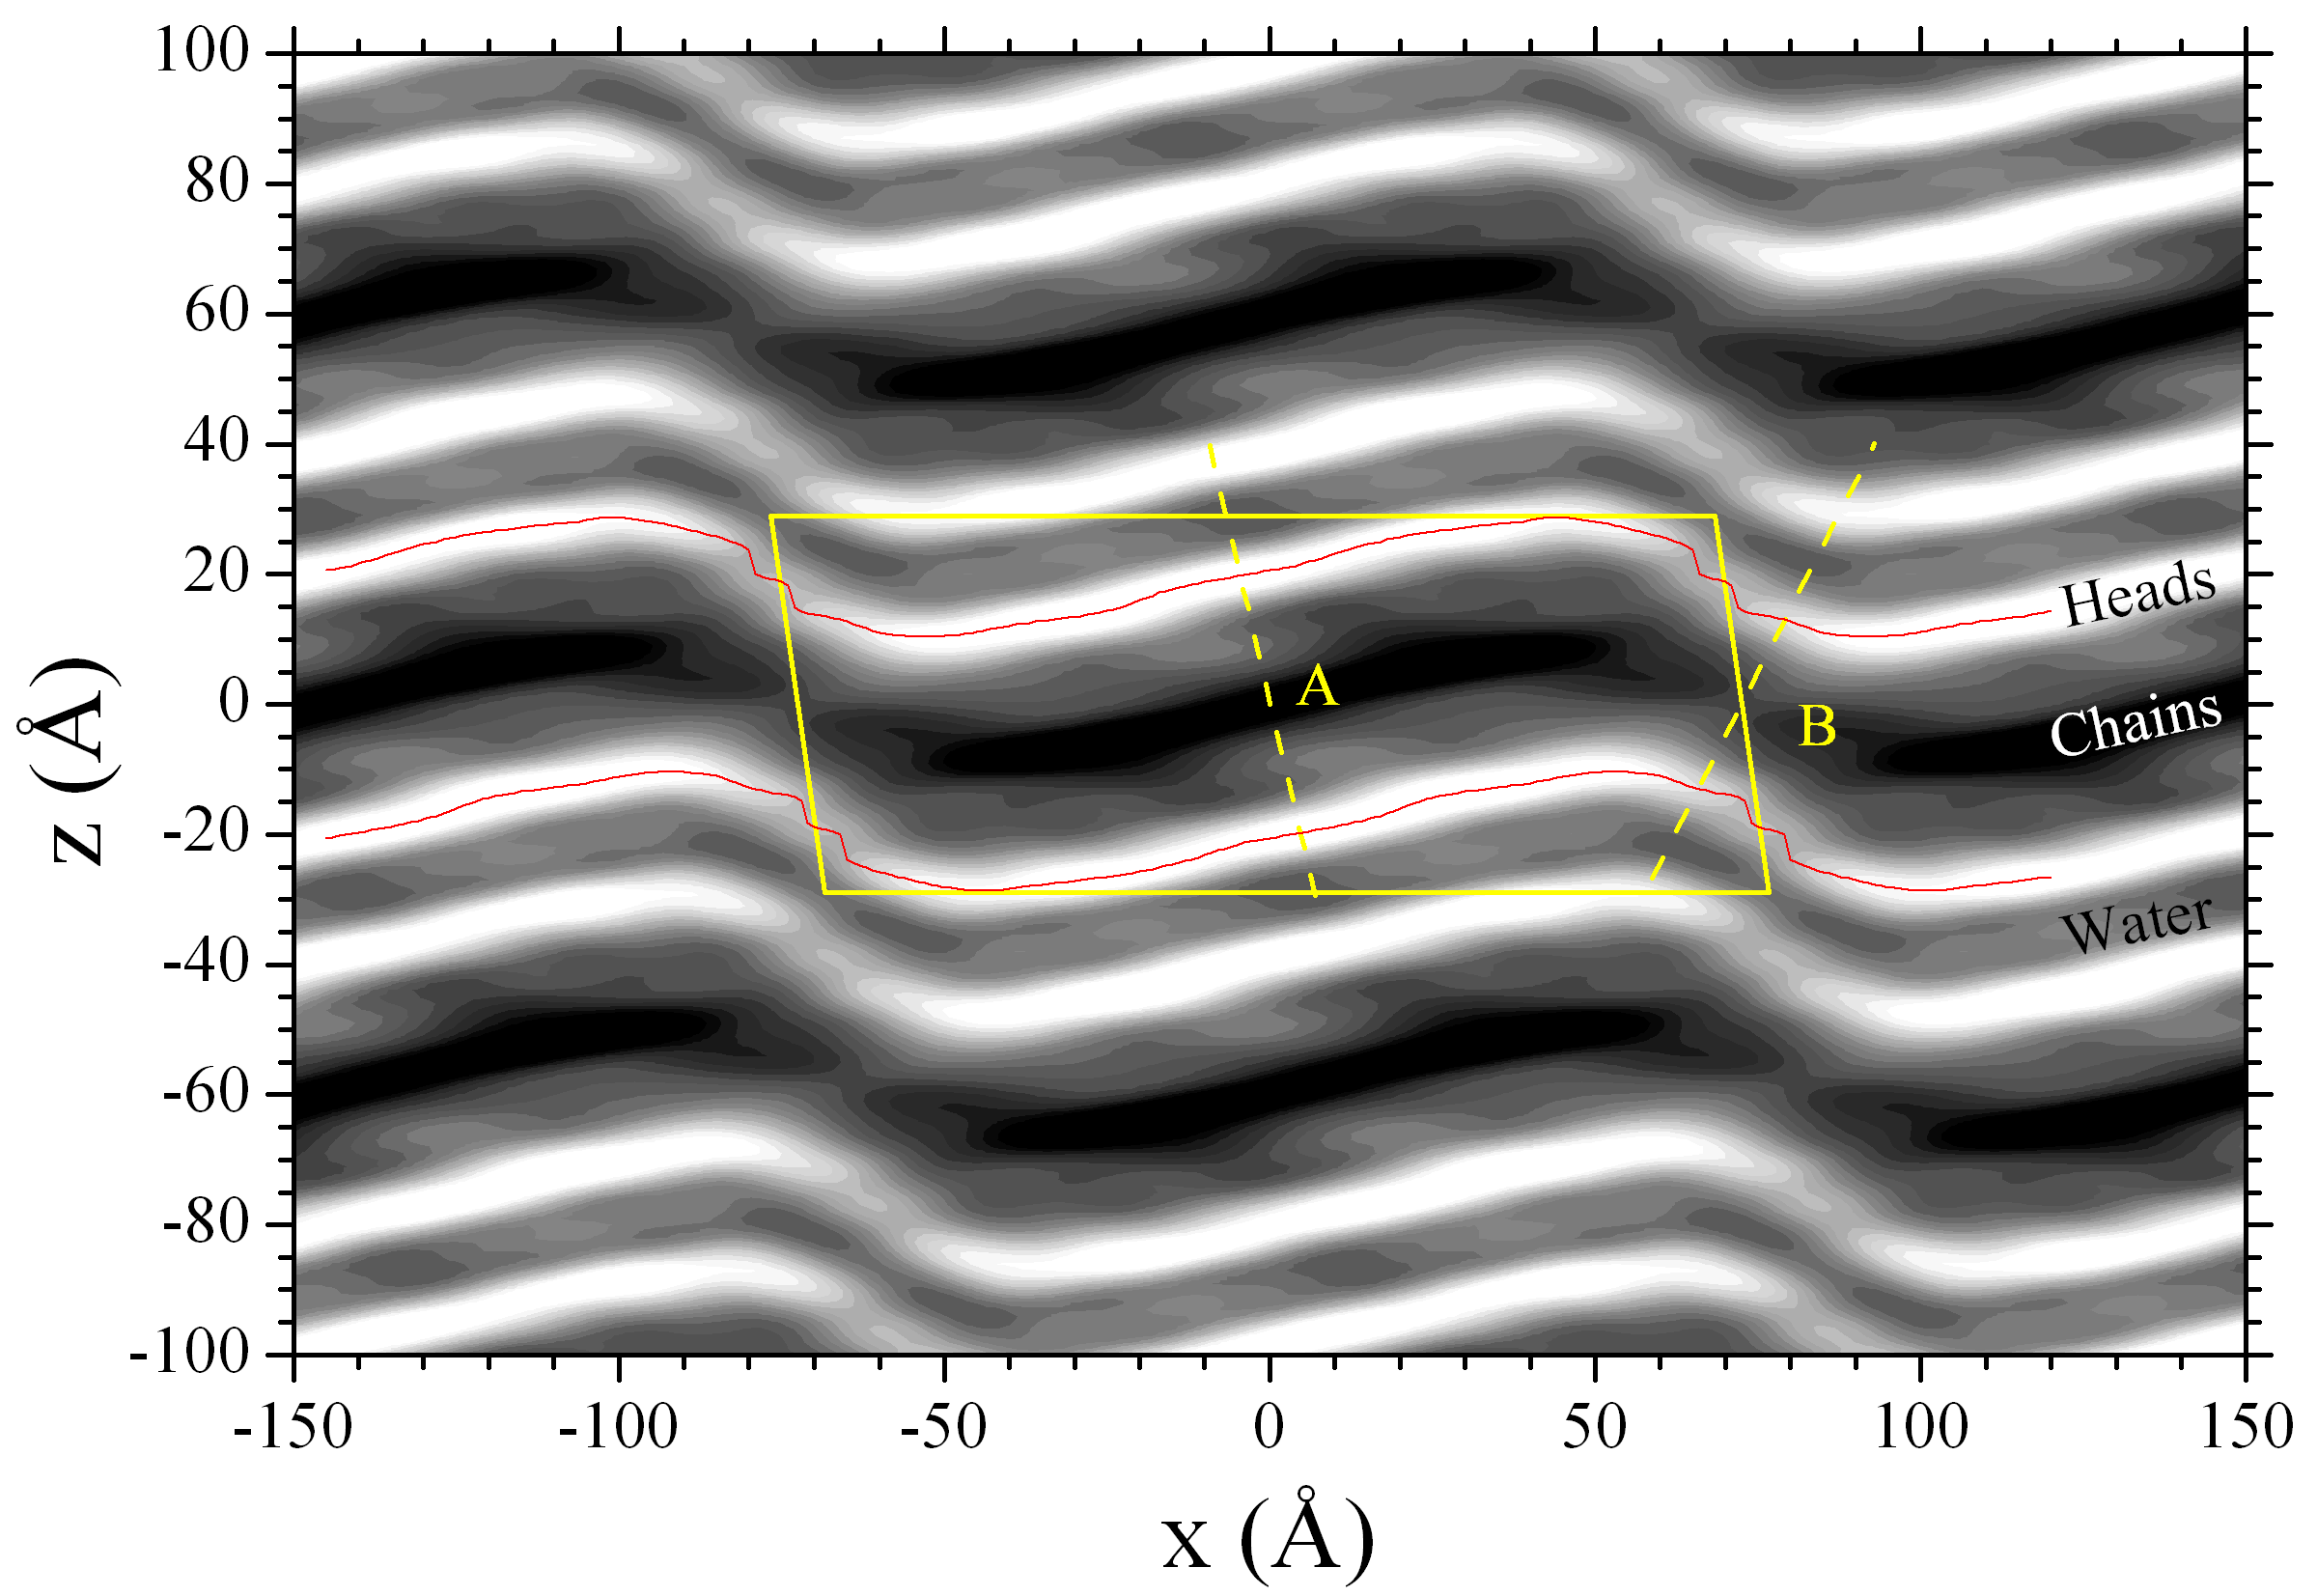
\includegraphics[width=0.9\textwidth]{figures/ripple/LAXS/Fit5_2D_edp}
  \caption[Two dimensional electron density profile calculated using the phases
  predicted by the 2G hybrid model (Fit5)]
  {Two dimensional electron density profile calculated using the phases
  predicted by the 2G hybrid model (Fit5). White is most electron dense
  and black is least electron dense. A unit cell is shown with a solid yellow 
  line. Dash lines A and B are the slices plotted in 
  Fig.~\ref{fig:major_diff_models} and Fig.~\ref{fig:minor_diff_models},
  respectively.}
  \label{fig:Fit5_2D_edp}
\end{figure}

\begin{figure}[htbp]
  \centering
  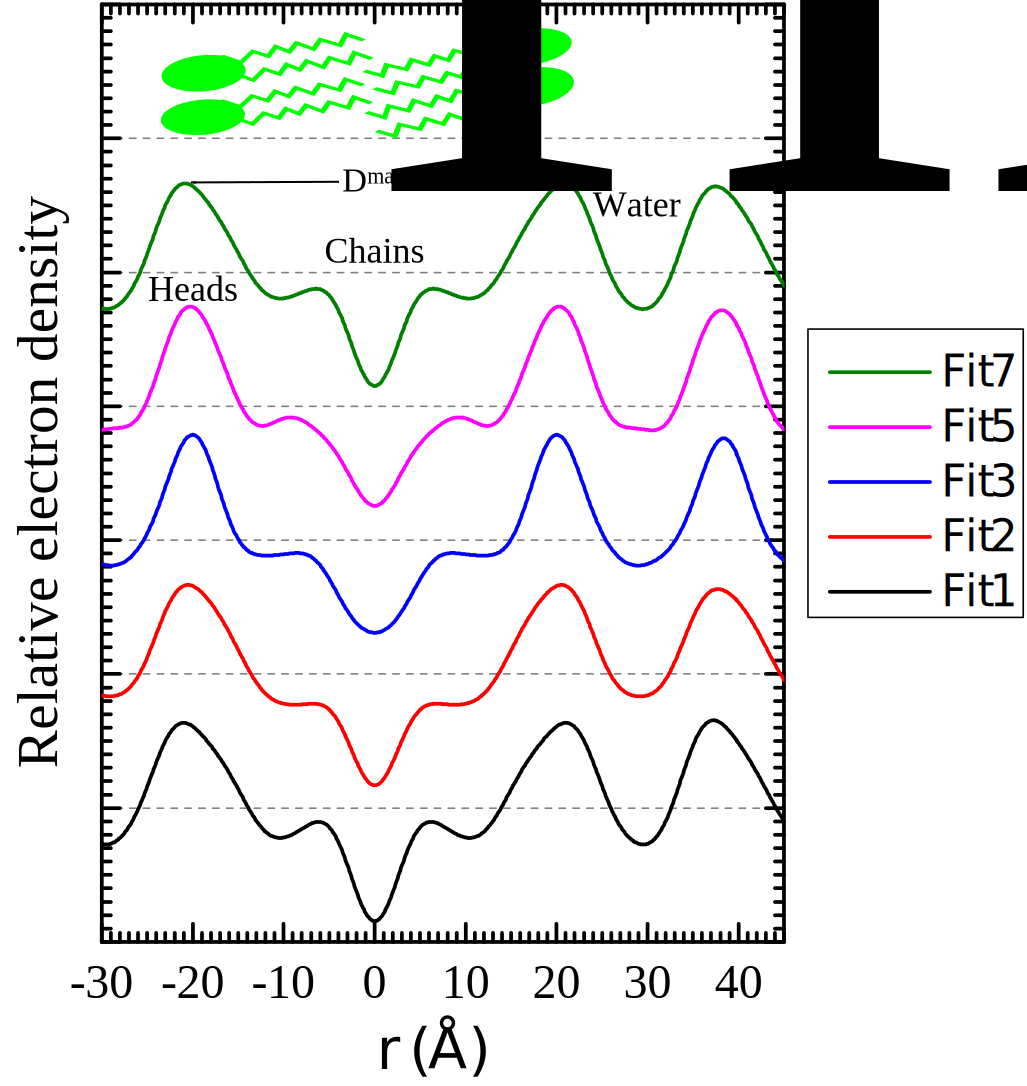
\includegraphics[width=0.9\textwidth]{figures/ripple/LAXS/major_diff_models}
  \caption{Electron density profiles along Slice A shown in Fig.~\ref{fig:Fit5_2D_edp}, 
  calculated using the phases
  predicted by different fits. The distance $r$ is measured from the bilayer 
  center. A cartoon of lipids is shown at the top, designating different parts of the profile
  as the lipid headgroup and chains. The fit from which each profile was calculated
  is shown in the figure legend.}
  \label{fig:major_diff_models}
\end{figure}

\begin{figure}[htbp]
  \centering
  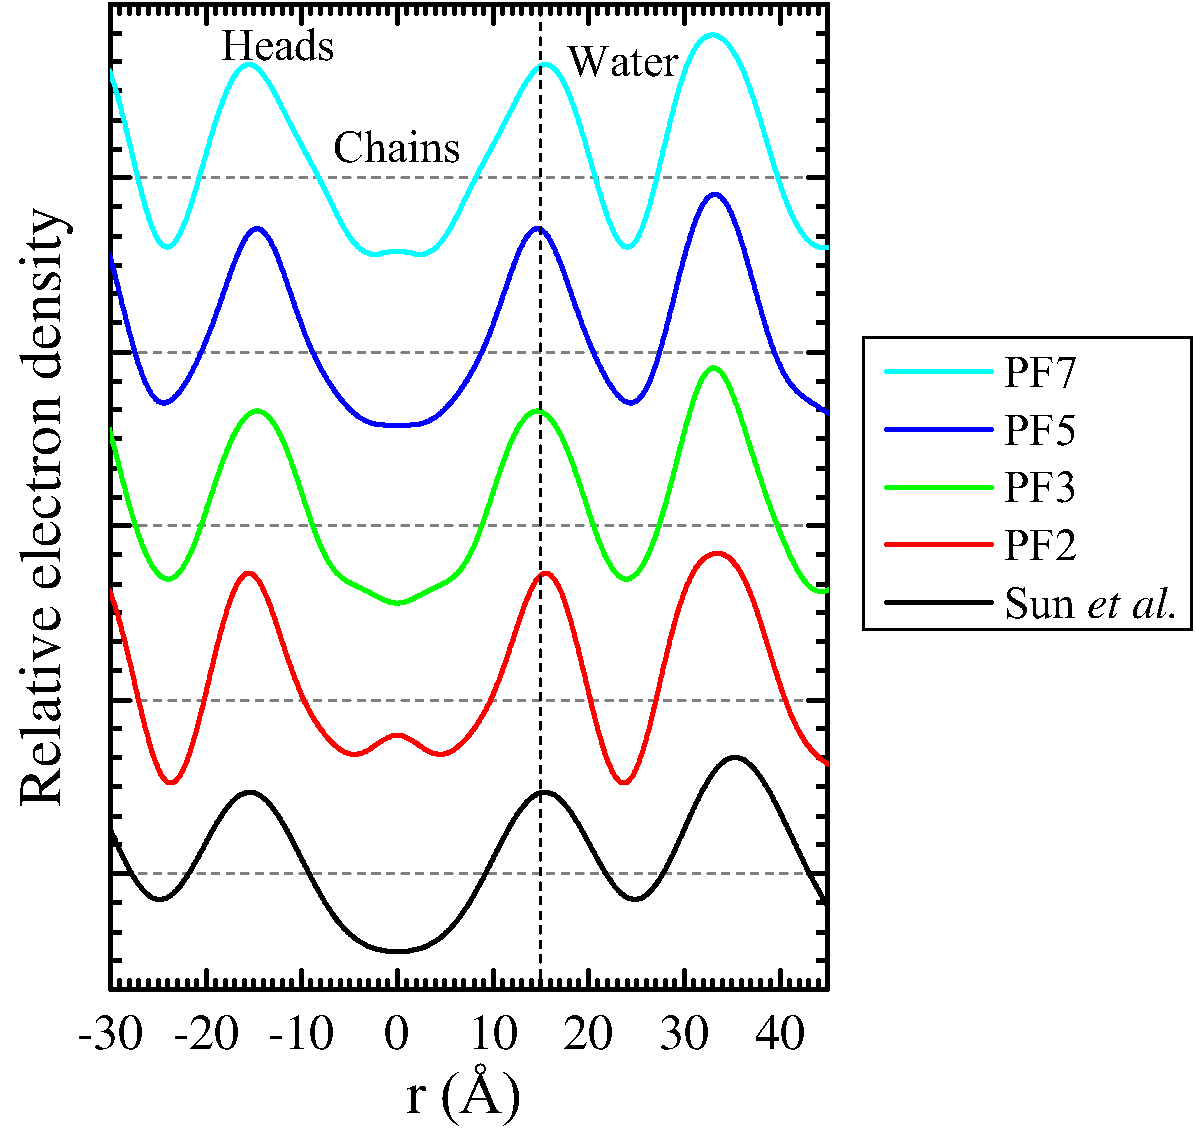
\includegraphics[width=0.9\textwidth]{figures/ripple/LAXS/minor_diff_models}
  \caption{Electron density profiles along Slice B shown in Fig.~\ref{fig:Fit5_2D_edp}, 
  calculated using the phases
  predicted by different fits. The distance $r$ is measured from the bilayer 
  center. The fit from which each profile was calculated
  is shown in the figure legend.}
  \label{fig:minor_diff_models}
\end{figure}

\begin{table}[htbp]
  \centering
  \begin{tabular}{cccccccccccc}
    \hline
          & Fit1  & Fit2  & Fit3  & Fit4  & Fit5  & Fit6  & Fit7 & I & II & III \\
    \hline
    $\chi^2$ & 11996 & 9664  & 19458 & 8827  & 8525  & 8905  & 8883 & & 1364 & 8131\\
    $D_\text{HH}^\text{major}$ & 42.0  & 41.0  & 40.0  & 40.6  & 40.6  & 41.8  & 41.8 & 38 & 38.0 & 41.8 \\
    $D_\text{HH}^\text{minor}$ & 30.8  & 31.0  & 29.2  & 29.2  & 29.2  & 31.0  & 31.0 & 31 & 28.6 & 30.6 \\
    $\alpha_M$ & 11.7\textdegree  & 11.5\textdegree  & 13.4\textdegree  & 11.7\textdegree  & 11.8\textdegree  & 11.8\textdegree  & 11.8\textdegree & 10.5\textdegree & 11.5\textdegree & 11.5\textdegree \\
    $\alpha_m$ & 23.7\textdegree  & 42.7\textdegree  & 22.9\textdegree  & 27.7\textdegree  & 27.1\textdegree  & 26.5\textdegree  & 26.9\textdegree & 26.1\textdegree & 28.1\textdegree & 25.1\textdegree \\
    \hline
  \end{tabular}
  \caption{Ripple structural quantities. \\
  I: Results from Sun \textit{et al.} \\
  II: Used only up to $(h,k)$ = (3, 4) \\ 
  III: Replaced lower order $|F_{hk}|$ with those from Wack and Webb, keeping the same relative error
  }
  \label{tab:LAXS_DHH}
\end{table}

\begin{figure}[htbp]
  \centering
  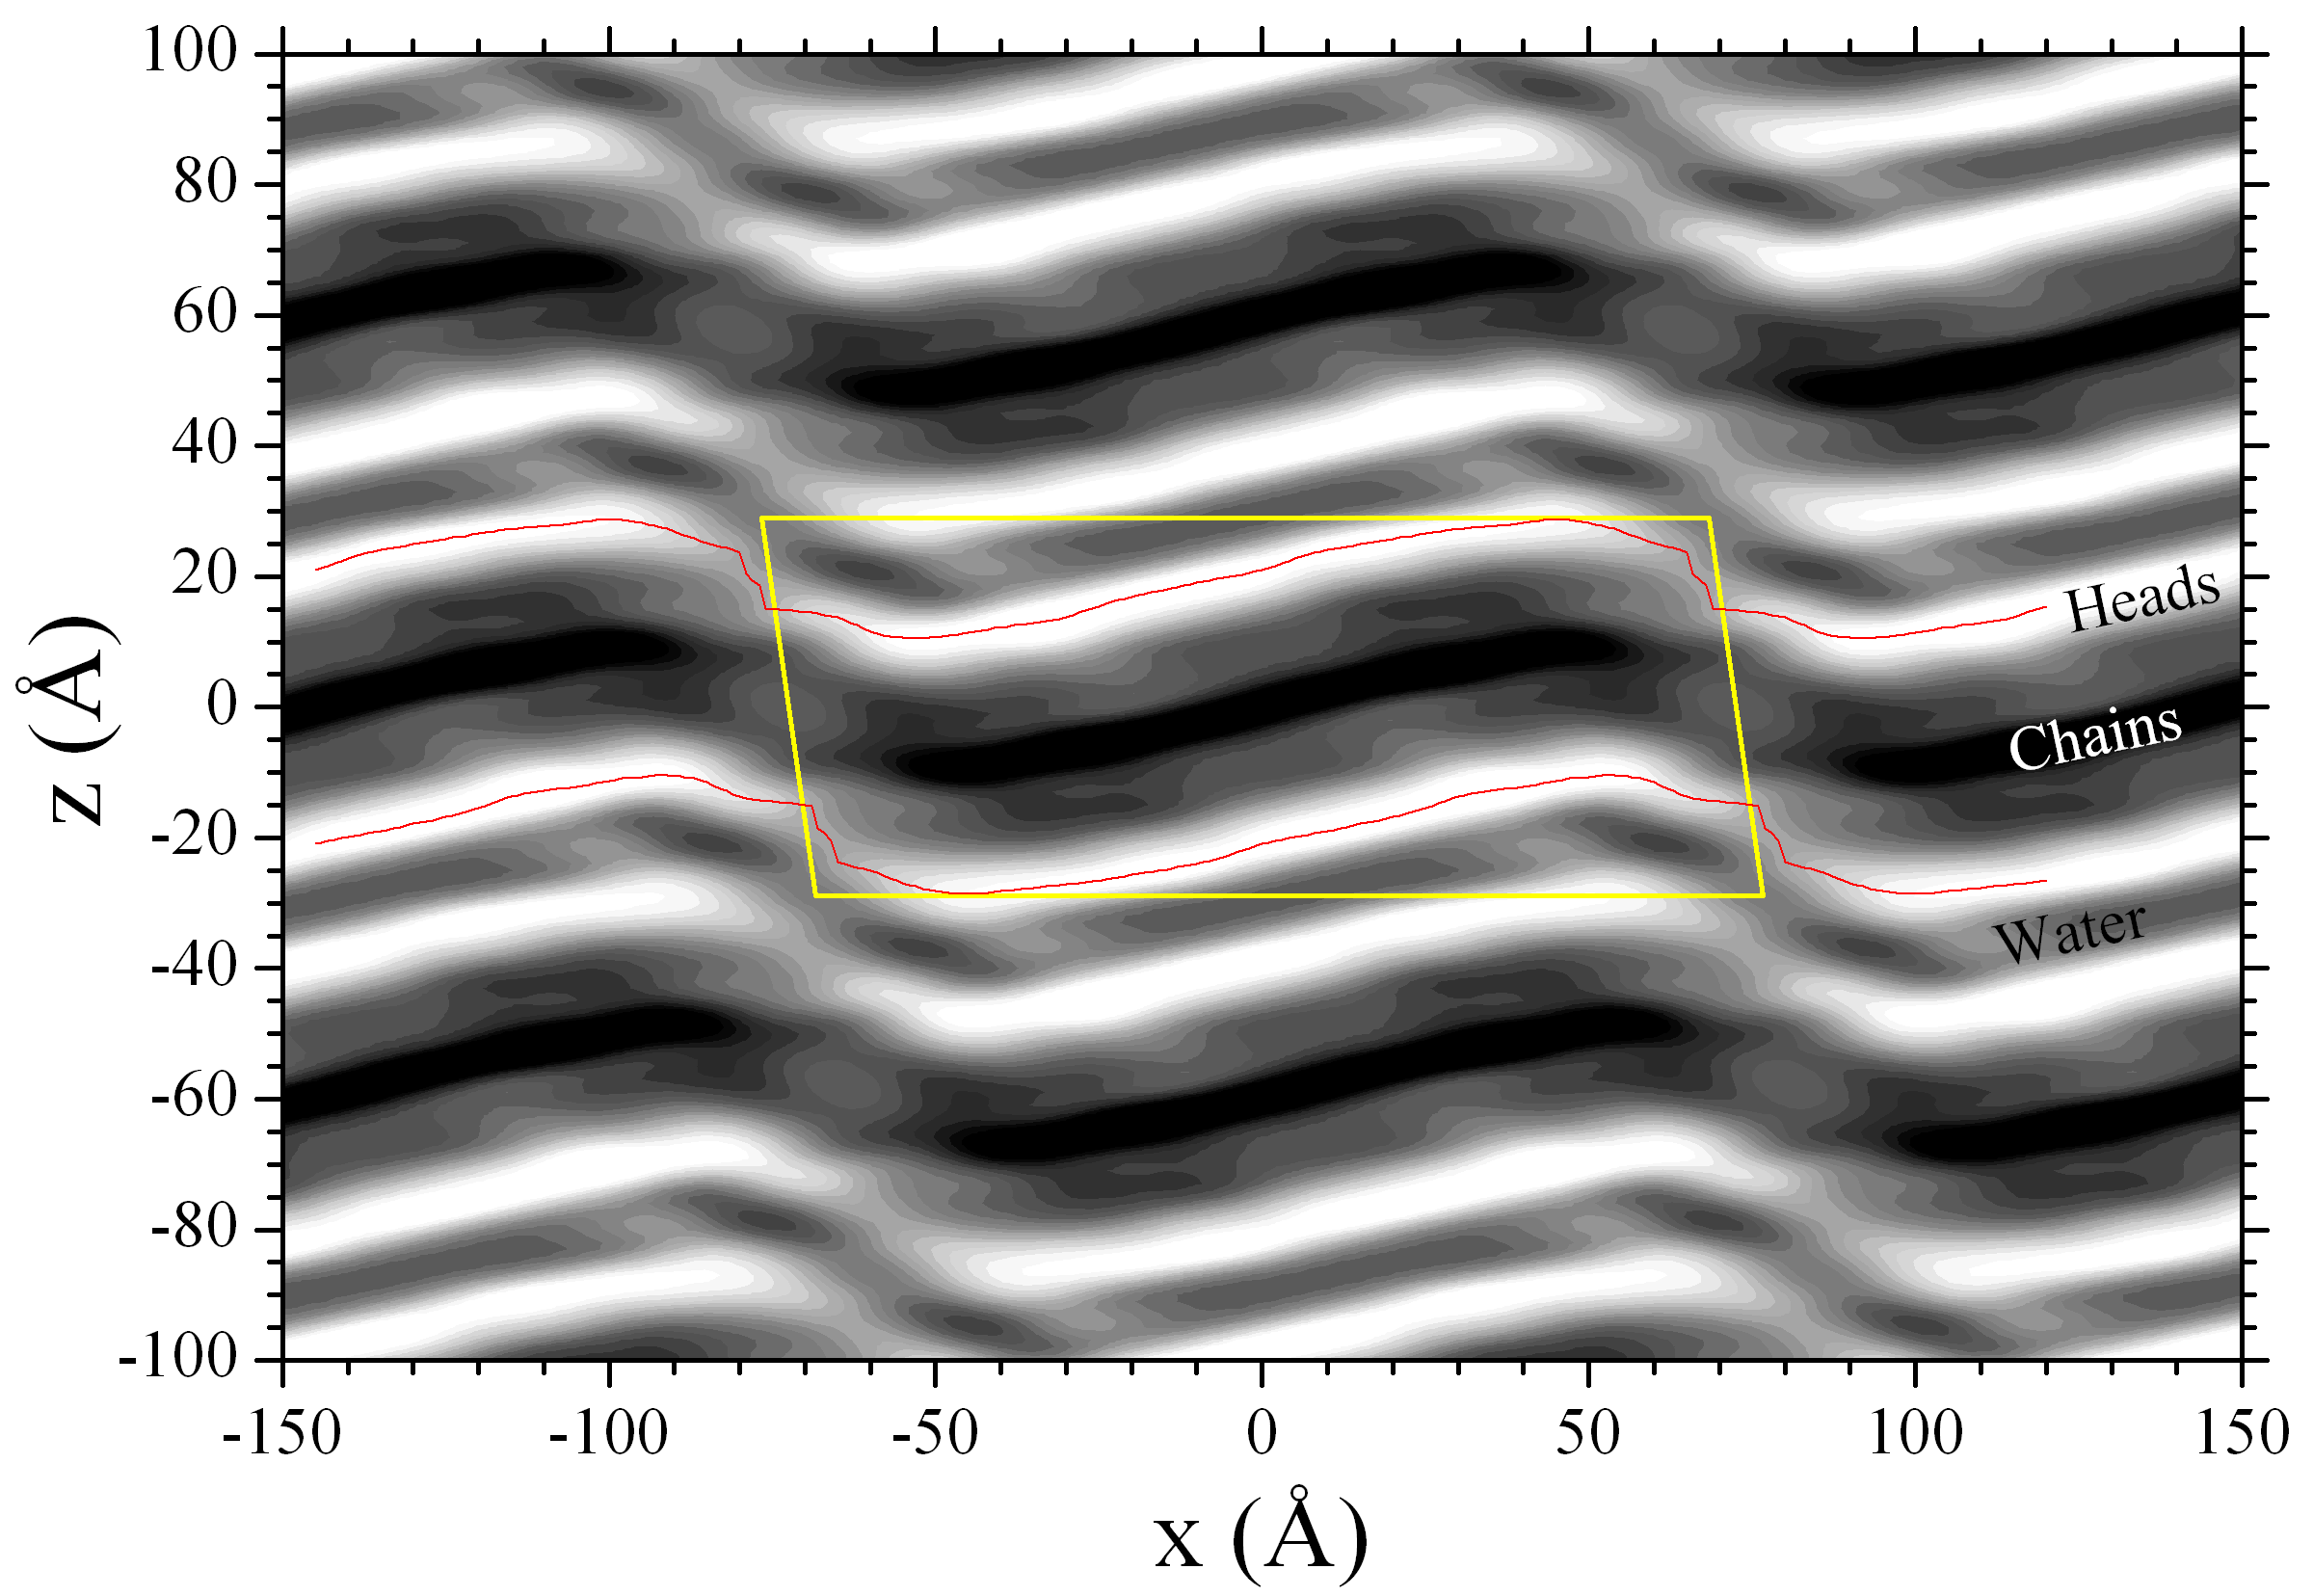
\includegraphics[width=0.9\textwidth]{figures/ripple/LAXS/Fit2_2D_edp}
  \caption[Two dimensional electron density map calculated using the phases
  predicted by Fit2]
  {Two dimensional electron density profile calculated using the phases
  predicted by Fit2.}
  \label{fig:Fit2_2D_edp}
\end{figure}

As noted in a previous paragraph, fits to ($h, k$) = (3, 0), (6, 0)--(6, 4),
and (9, 0) were not great. We also noticed that the phase of (1, 3) was unstable. To study
how the electron density profile varies as we vary the phases of those peaks,
we deliberately reversed the sign of the phases. Figure~\ref{fig:major_phase_variation}
and \ref{fig:minor_phase_variation} show the effect of such operations
starting with the phases obtained by Fit5. 
In Fit5a, we inverted the phase of (3, 0) and in Fit5b, the phases of 
(1, 3), (3, 0), (6, 0), and (9, 0) were inverted.
In Fit5c, we further reversed the sign of (6, 1--4) from Fit5b.
Essentially, we obtained approximately the same $D_\text{HH}^\text{major}$
among three cases. In contrast, the variation in $D_\text{HH}^\text{minor}$ was
larger, and in Fit5c, $D_\text{HH}^\text{minor}$ = 31.8 \AA.
Also, presence of the terminal methyl trough in the major arm was robust, but
the profile of the chain regions in the minor arm was not.

\begin{figure}[htbp]
  \centering
  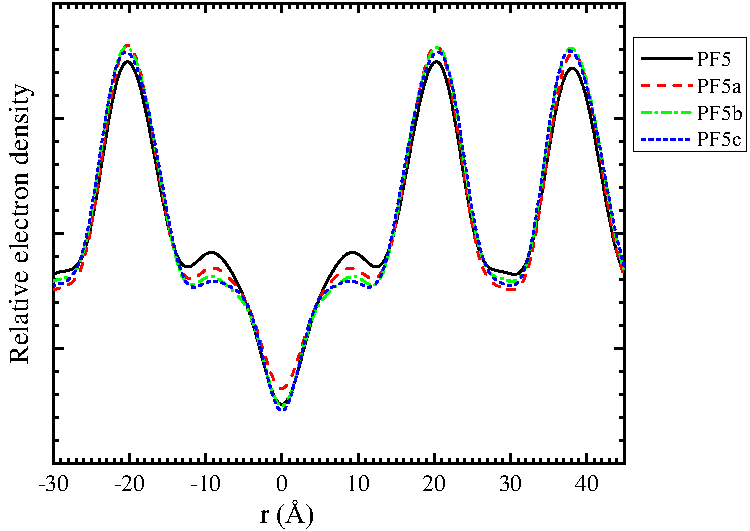
\includegraphics[width=0.7\textwidth]{figures/ripple/LAXS/major_phase_variation}
  \caption{Variation in the electron density profile along Slice A. 
  Reversing the sign of the (3, 0) phase in Fit5 
  resulted in the red dashed profile (Fit5a). Reversing the sign of the 
  (1, 3), (3, 0), (6, 0), and (9, 0) resulted in the green dash-dotted profile
  (Fit5b). Reversing the sign of the (1, 3), (3, 0), (6, 0--4), and (9, 0)
  resulted in the blue short dashed profile (Fit5c). 
  The distance $r$ is measured from the bilayer center.}
  \label{fig:major_phase_variation}
\end{figure}

\begin{figure}[htbp]
  \centering
  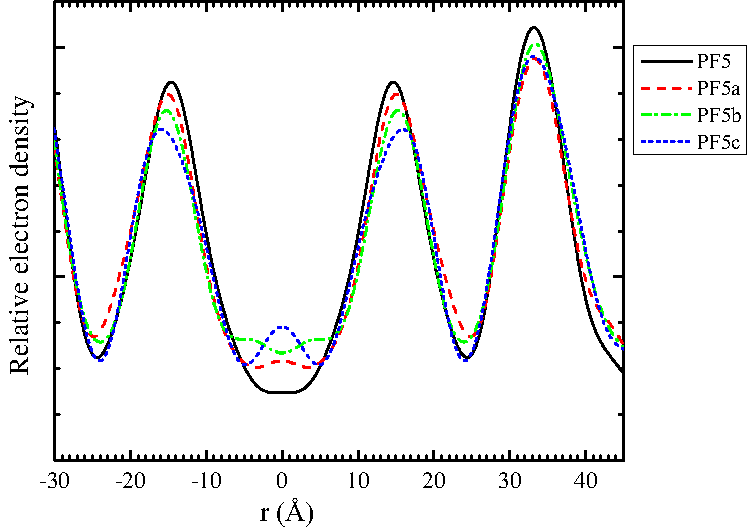
\includegraphics[width=0.7\textwidth]{figures/ripple/LAXS/minor_phase_variation}
  \caption{Variation in the electron density profile along Slice B.
  Reversing the sign of the (3, 0) phase in Fit5 
  resulted in the red dashed profile (Fit5a). Reversing the sign of the 
  (1, 3), (3, 0), (6, 0), and (9, 0) resulted in the green dash-dotted profile
  (Fit5b). Reversing the sign of the (1, 3), (3, 0), (6, 0--4), and (9, 0)
  resulted in the blue short dashed profile (Fit5c). 
  The distance $r$ is measured from the bilayer center.}
  \label{fig:minor_phase_variation}
\end{figure}

In summary, we observed that the thickness of the minor arm was 
smaller than that of the major arm and these thicknesses did not vary 
much among different models and fits. 
The electron density profile in the major 
arm showed clear separation of the headgroup and chains while that in the minor 
arm did not. 
Furthermore, the terminal methyl trough like feature in the major arm was 
quite robust, but 
whether the minor arm has a small dip or rise in the density at the bilayer center
could not be determined. 
Obtaining a robust electron density profile in the minor
arm may require an improved model. Table~\ref{tab:LAXS_summary} summarizes
the final structural results.

\begin{table}[htbp]
  \centering
  \begin{tabular}{cc}
    \hline
    $\xM$ & 101 $\pm$ 2 \AA \\
    $A$ & 21 $\pm$ 1 \AA \\
    $D_\text{HH}^\text{major}$ & 41 $\pm$ 1 \AA \\
    $D_\text{HH}^\text{minor}$ & 30.5 $\pm$ 1.5 \AA \\
    $\alpha_M$ & 12\textdegree\ $\pm$ 1\textdegree \\
    $\alpha_m$ & 27\textdegree\ $\pm$ 1\textdegree \\
    $D$ & 57.8 \AA \\
    $\lambda_r$ & 145.0 \AA \\
    $\gamma$ & 98.2\textdegree \\
    \hline
  \end{tabular}
  \caption{Estimated structural quantities}
  \label{tab:LAXS_summary}
\end{table}

\begin{figure}
  \centering
  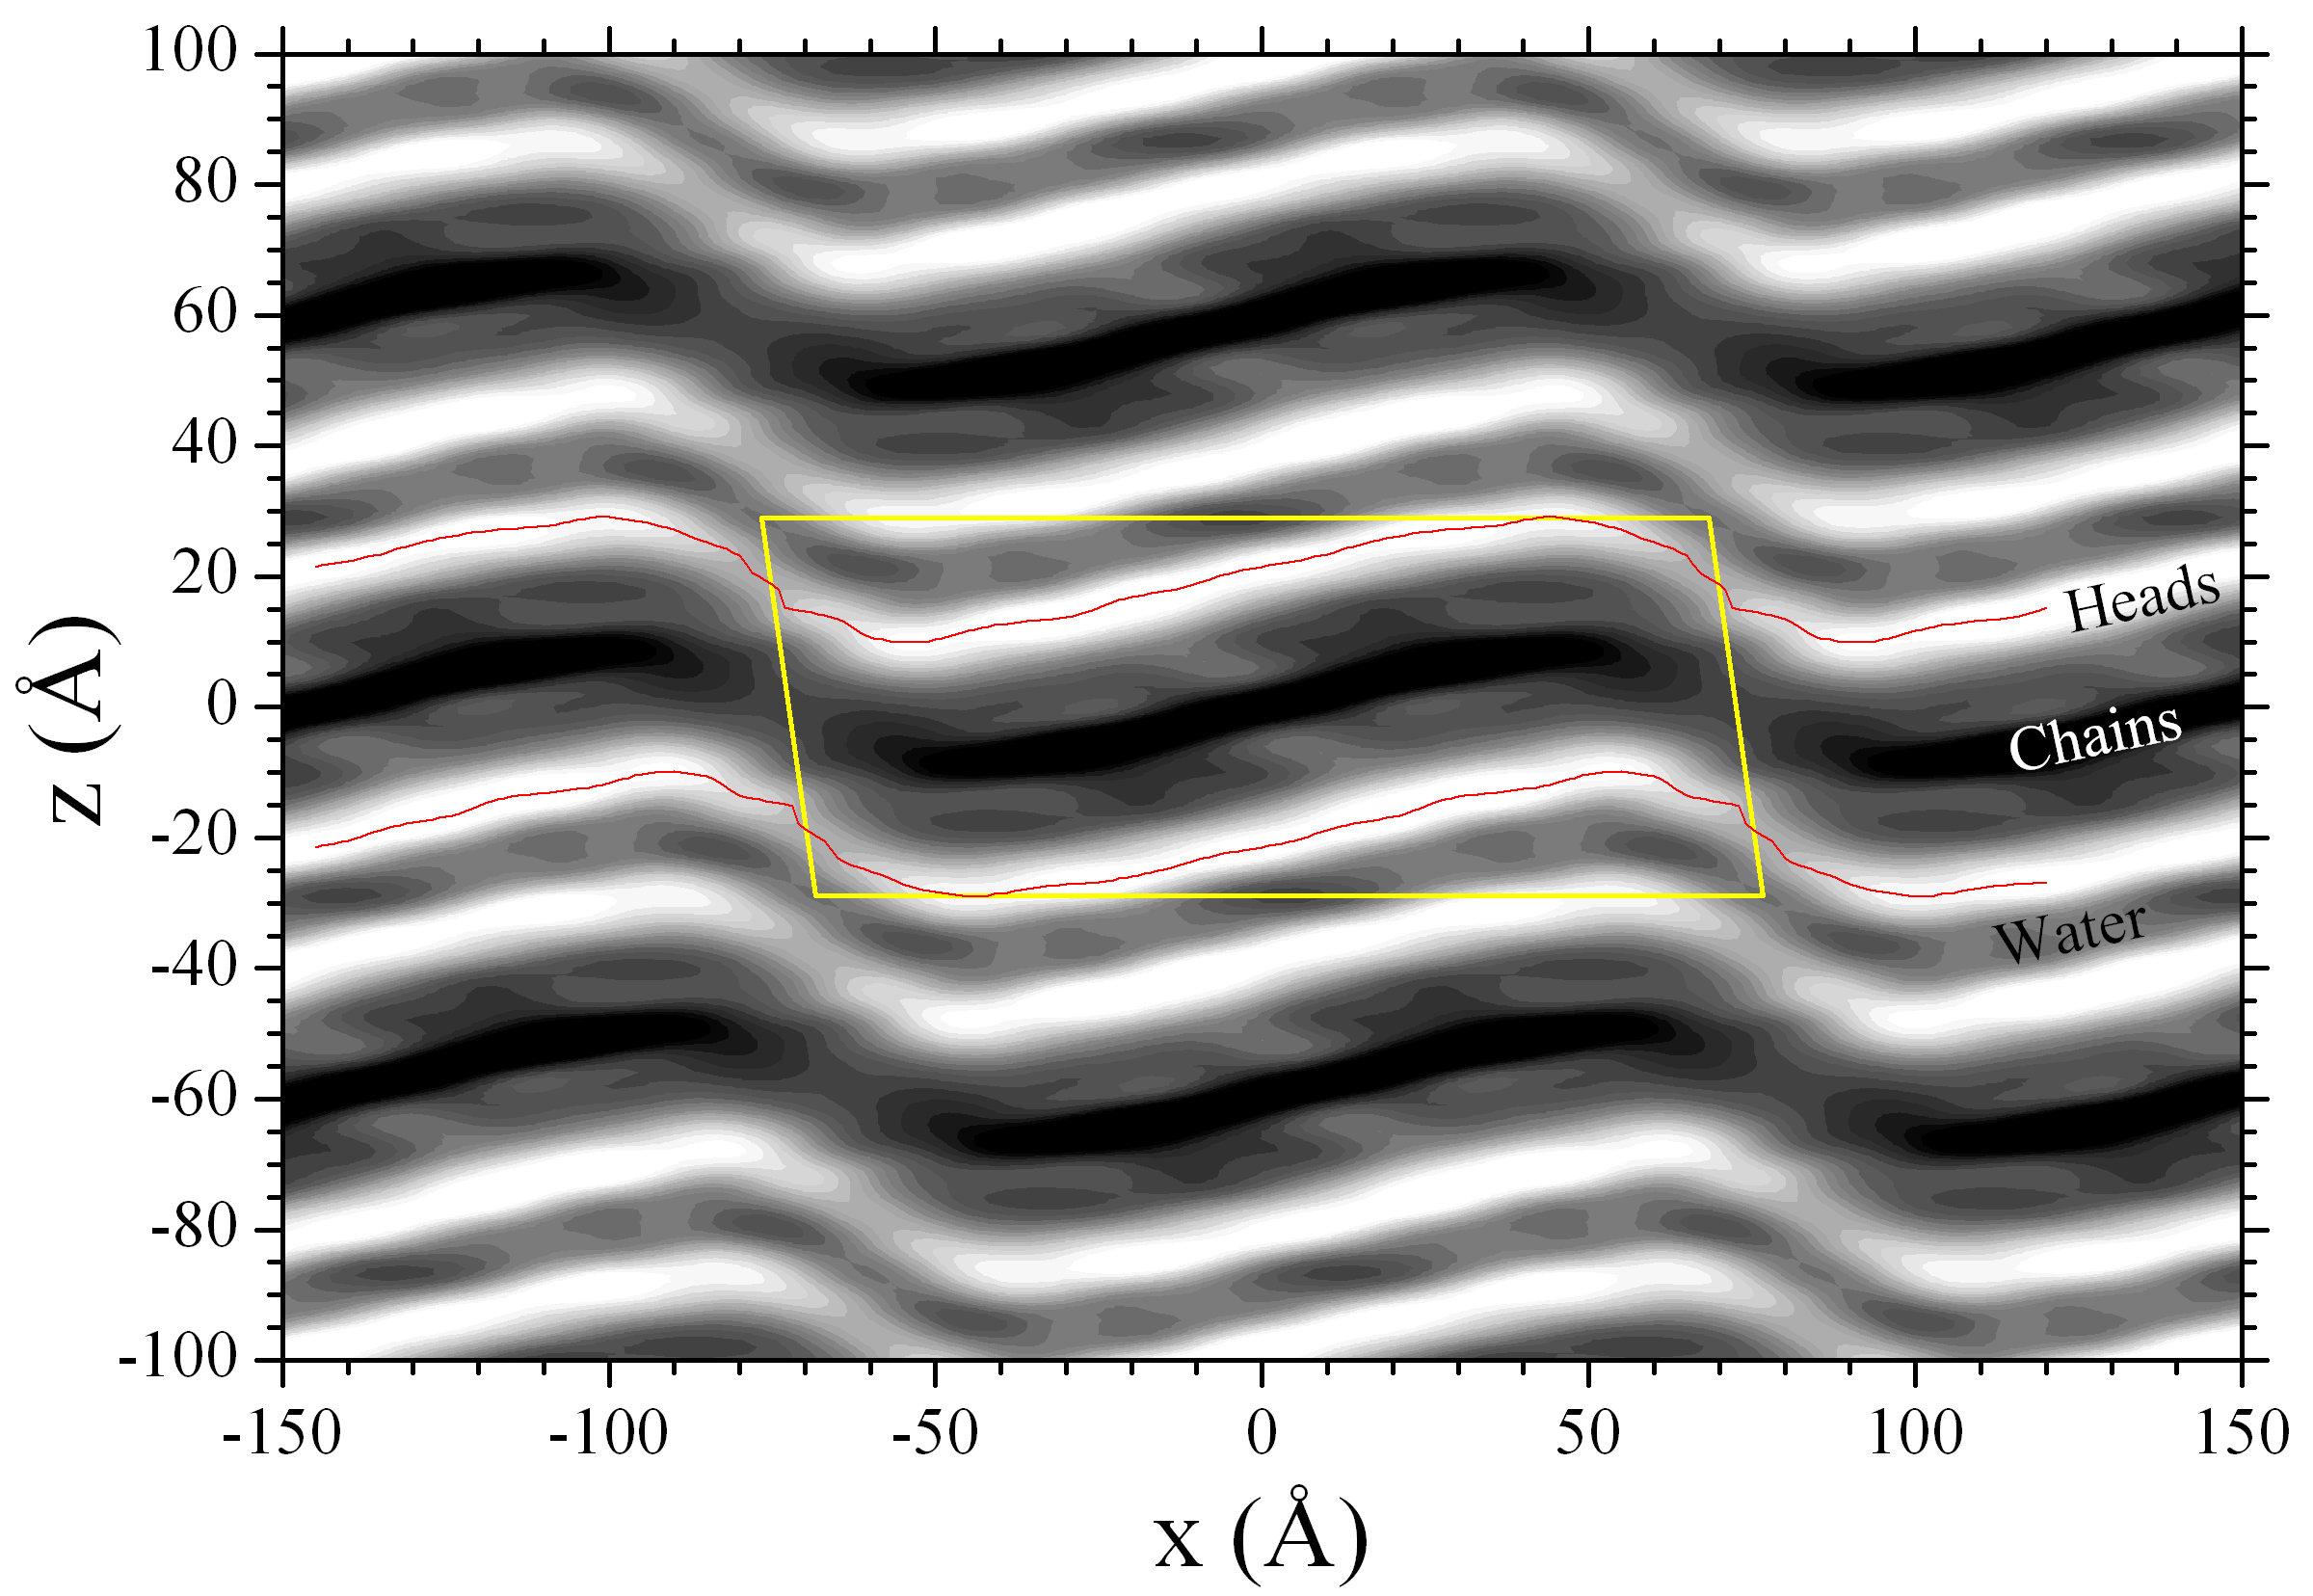
\includegraphics[width=0.9\textwidth]{figures/ripple/LAXS/Fit1_2D_edp}
  \caption[]{Two dimensional electron density map calculated using the phases
  predicted by Fit1}
  \label{fig:Fit1_2D_edp}
\end{figure}

\begin{figure}
  \centering
  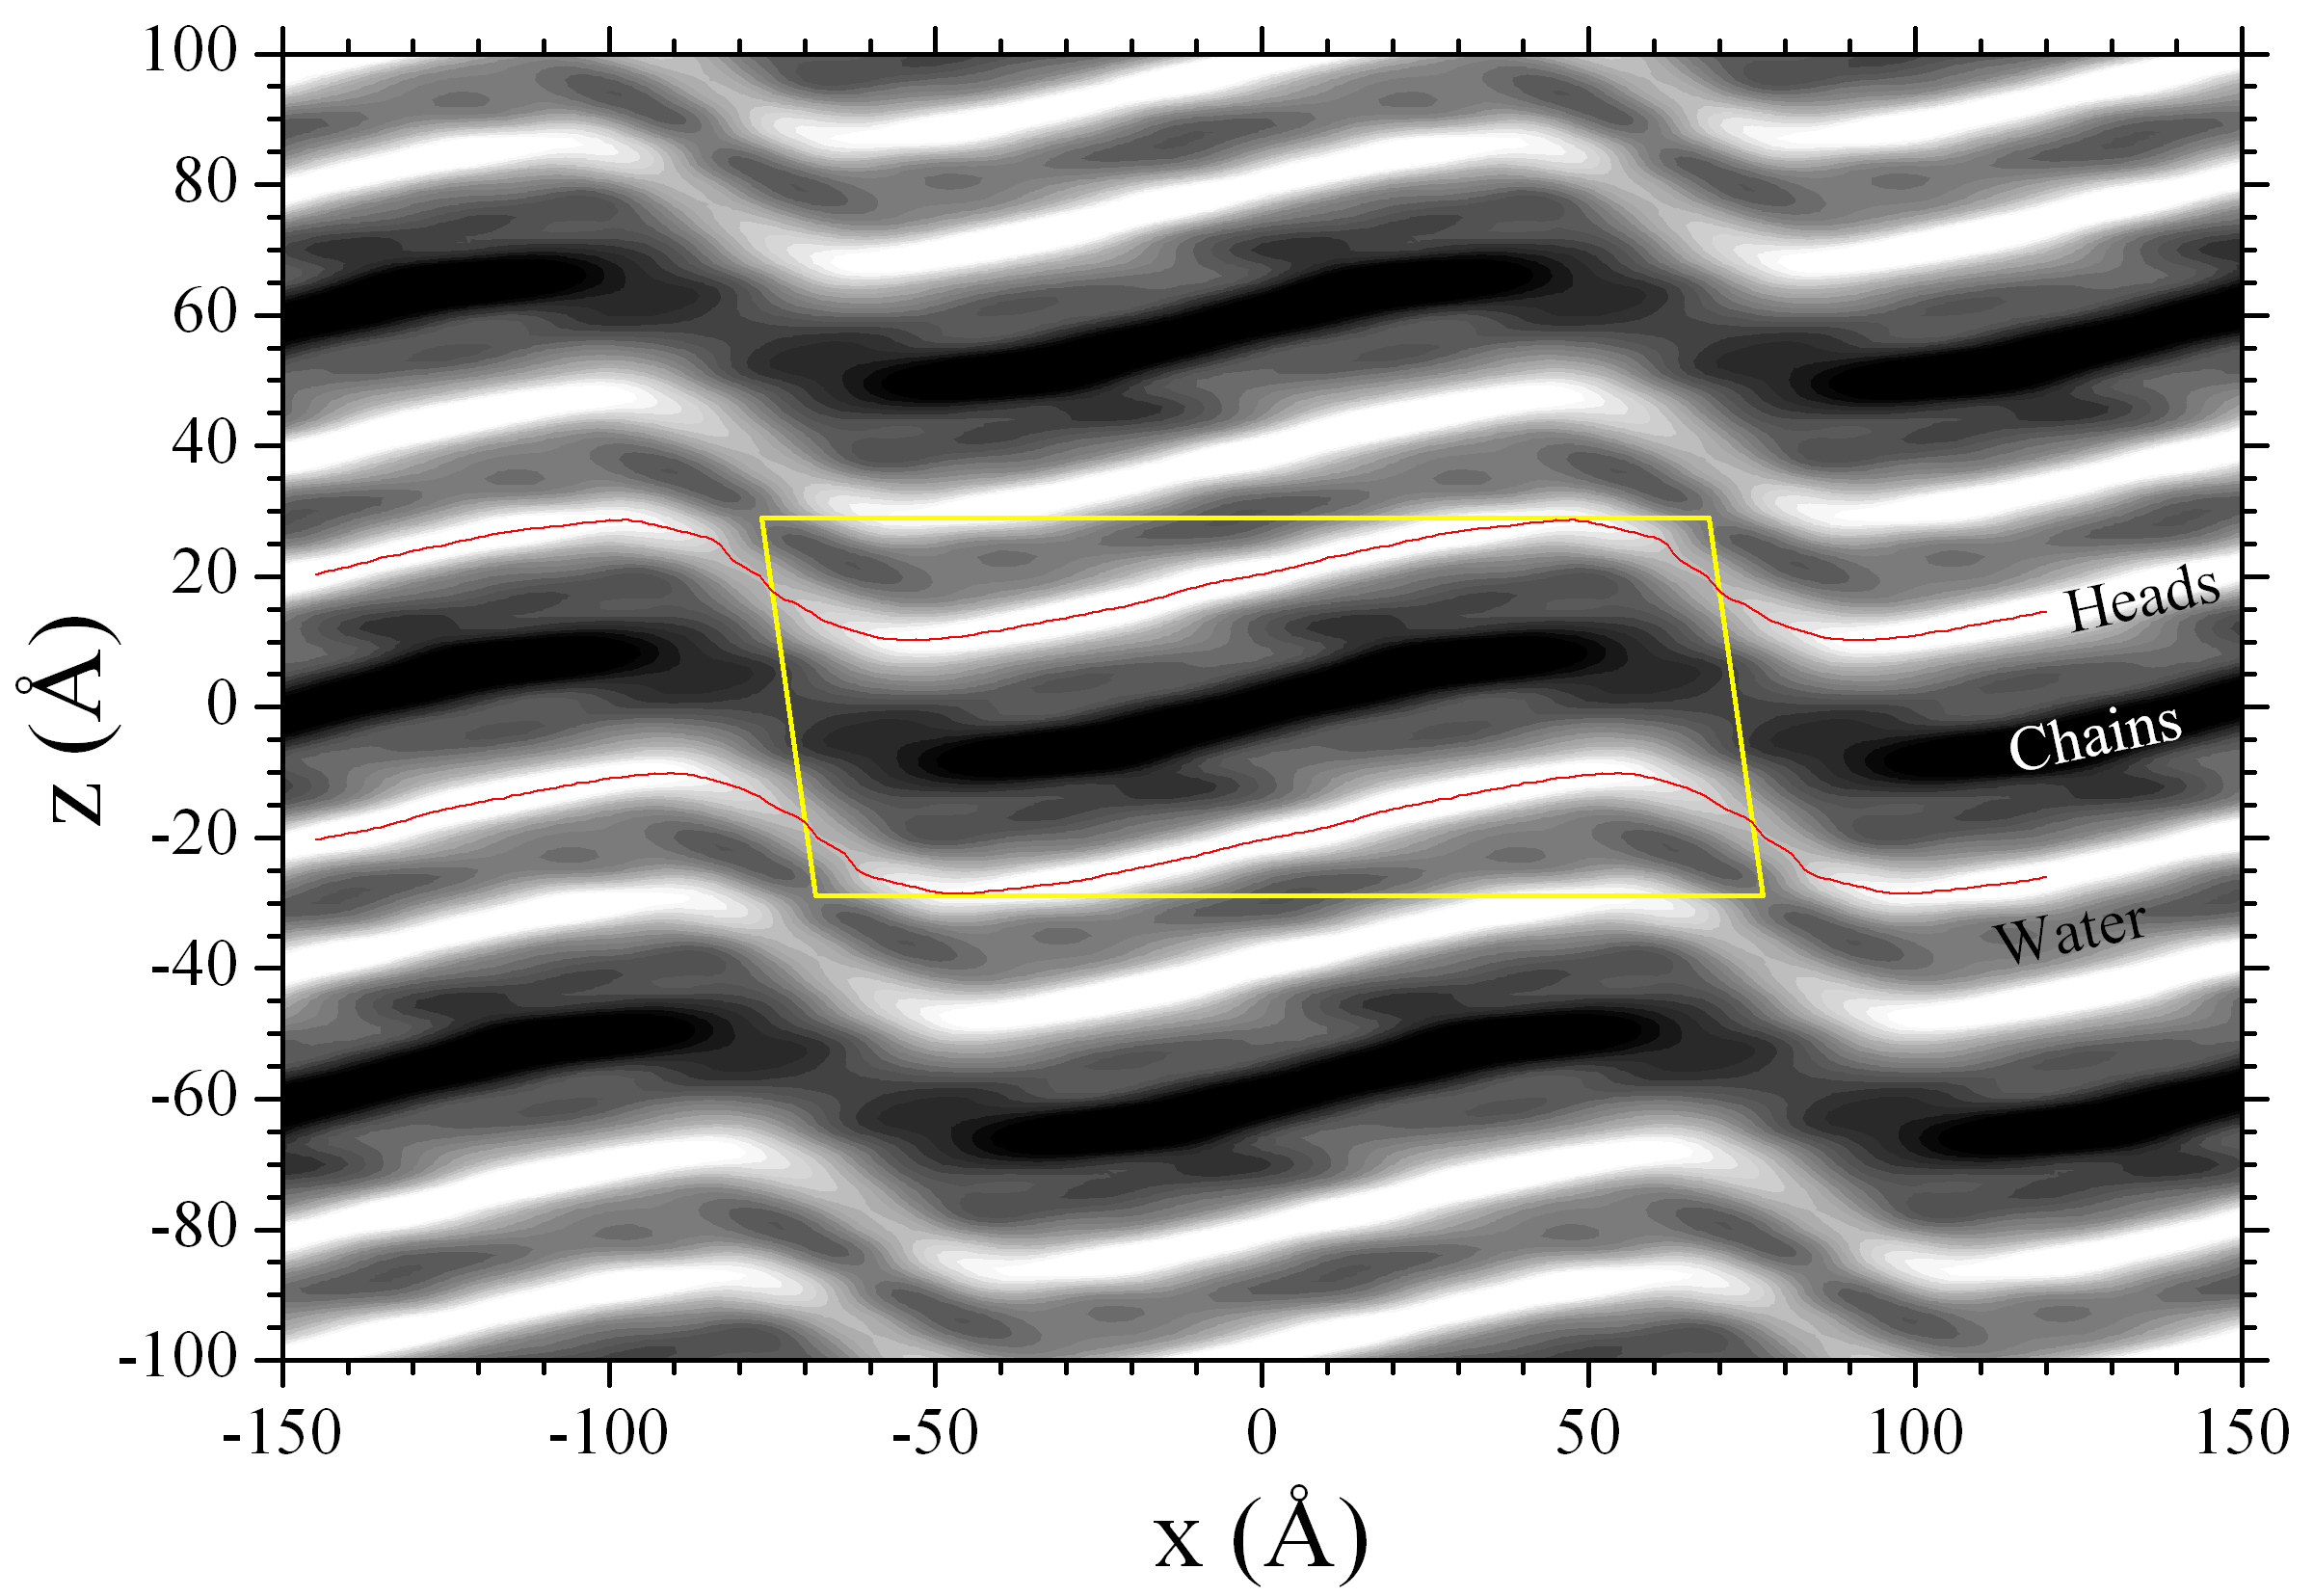
\includegraphics[width=0.9\textwidth]{figures/ripple/LAXS/Fit3_2D_edp}
  \caption[]{Two dimensional electron density map calculated using the phases
  predicted by Fit3}
  \label{fig:Fit3_2D_edp}
\end{figure}

\begin{figure}
  \centering
  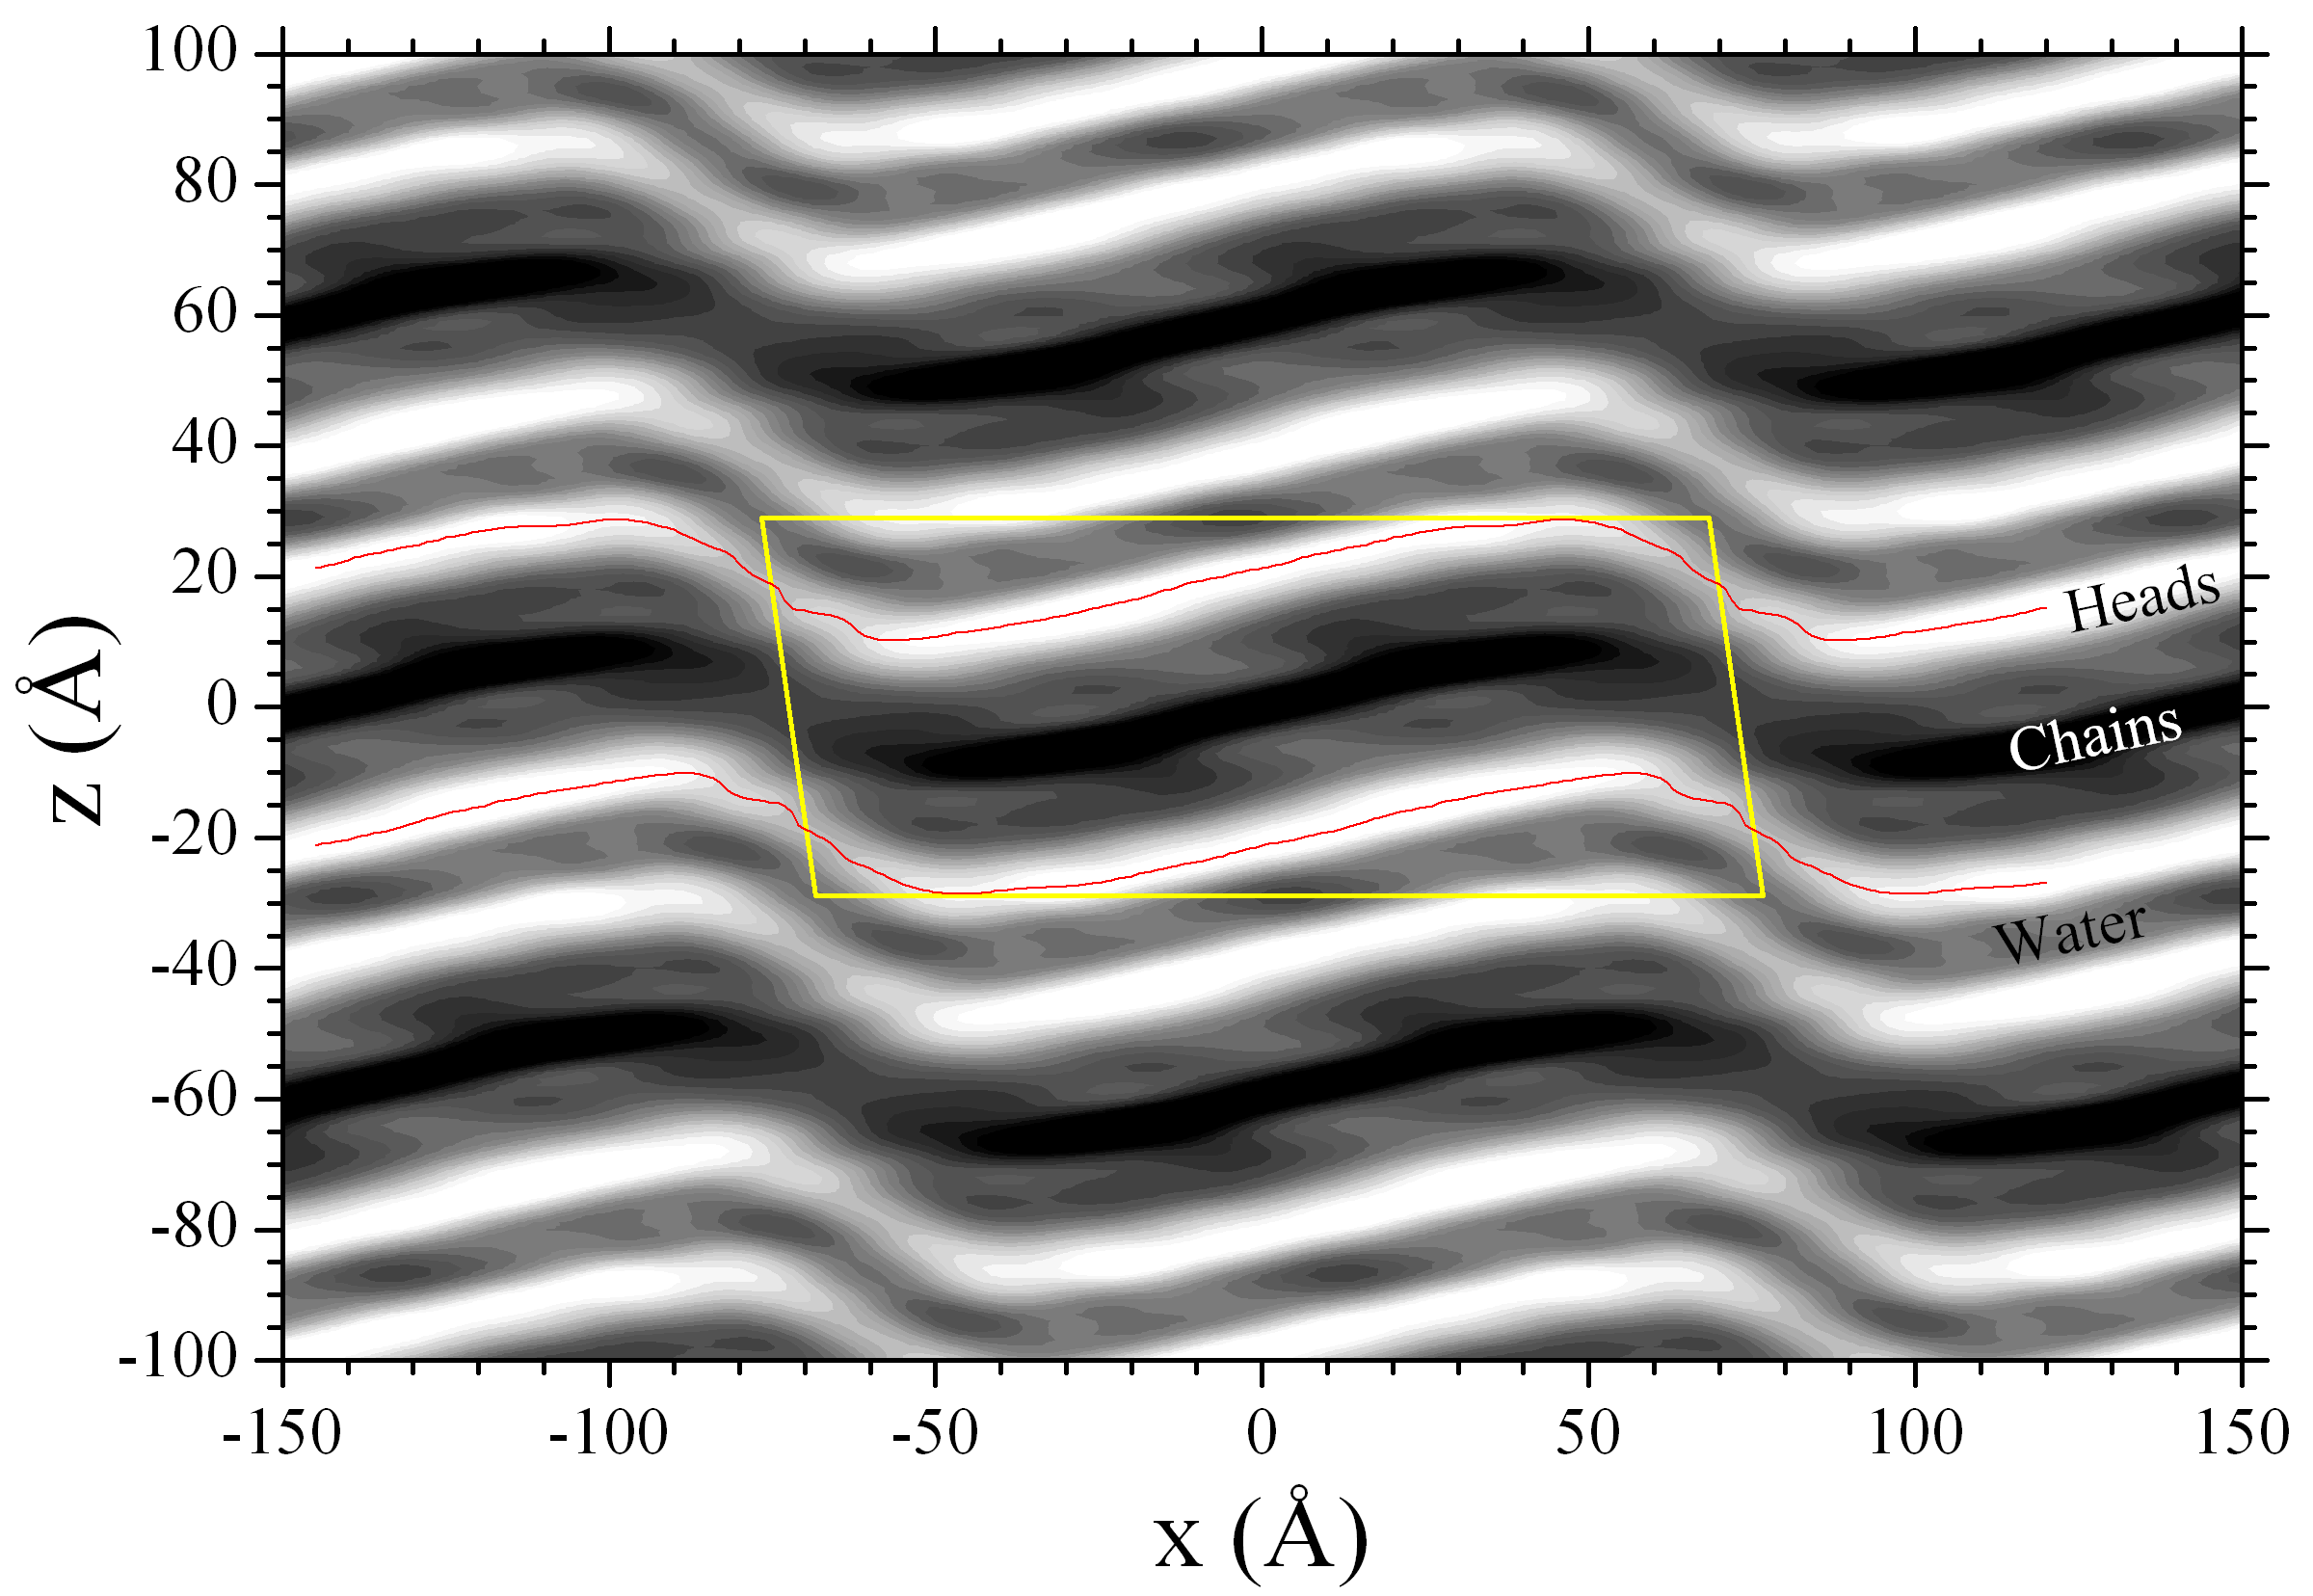
\includegraphics[width=0.9\textwidth]{figures/ripple/LAXS/Fit7_2D_edp}
  \caption[]{Two dimensional electron density map calculated using the phases
  predicted by Fit7}
  \label{fig:Fit7_2D_edp}
\end{figure}

%%%%%%%%%%%%%%%%%%%%%%%%%%%%%%%%%%%%%%%%%%%%%%%%%%%%%%%%%%%%%%%%%%%%%%%%%%%%%%%
%\section{nGIWAXS: analysis}
%\subsection{Absorption Correction}\label{sec:WAXS_abs_correction}
%(Under construction)

%%%%%%%%%%%%%%%%%%%%%%%%%%%%%%%%%%%%%%%%%%%%%%%%%%%%%%%%%%%%%%%%%%%%%%%%%%%%%%%
%\section{nGIWAXS: model}
%\subsection{Thin rod model}\label{sec:WAXS_thin_rod}


%%%%%%%%%%%%%%%%%%%%%%%%%%%%%%%%%%%%%%%%%%%%%%%%%%%%%%%%%%%%%%%%%%%%%%%%%%%%%%%
\newpage
\section{nGIWAXS: results}\label{sec:nGIWAXS_results}
\subsection{Fluid and gel phase}\label{sec:nGIWAXS_fluid_gel_phase}
Figure~\ref{fig:waxs_data_reduction} shows the data reduction of 
near grazing incidence wide angle X-ray scattering (nGIWAXS) data of
the DMPC fluid phase at $T$ = 30 \textcelsius.
The original scattering image taken at $\omega=0.5$\textdegree\ had unwanted
scattering due to mylar windows in the hydration chamber which
overlapped with the fluid phase WAXS.
Subtracting background scattering data taken at incident angle $-\omega$  
removed these unwanted features in the scattering data, 
resulting in a sample scattering image 
(Fig.~\ref{fig:waxs_data_reduction}(bottom, left panel)).
This sample scattering image was then transformed to the
sample $q$-space using the relationship between the CCD 
pixel positions and the sample $q$-space
given by Eq.~\ref{eq:qxqyqz} and Eq.~\ref{eq:XZ}. The nonlinearity of this
relationship is
not negligible and must be taken into account for wide angle scattering data.
The black regions in the sample $q$-space image
(Fig.~\ref{fig:waxs_data_reduction}(bottom, right panel))
are the regions of $q$-space that
were not probed by the detector. Because of the nonlinearity in the 
transformation, straight detector edges were turned into curves, the effect of
which was most visible near the meridian $q_r$ = 0. All nGIWAXS data
in this chapter were reduced in the same manner.

Because of chain disordering in the fluid phase, chain-chain scattering
gives rise to intensity along an arc \cite{ref:Mills08} with a broad
width in $q$. 
Scattering of the fluid phase WAXS
is most intense at the equator. However, scattering near the equator
was strongly absorbed by the sample and substrate, so observing the 
peak in the fluid phase WAXS would require a different experimental 
geometry.
The data were collected with a low resolution setup to maximize
intensity. The low resolution did not pose a problem for analysis of the 
data because observed features were broad.
Figure~\ref{fig:fluid_qr} plots intensity along $q_r$ showing that
the fluid phase WAXS was centered at $q \approx$ 1.41 \AA$^{-1}$. 
This corresponds to an average chain-chain distance of 4.5 \AA. 
A Lorentzian fit to the profile resulted in the full width half maximum
(FWHM) $\Delta q_r=0.288$ \AA$^{-1}$.

\begin{figure}[htbp]
  \centering
  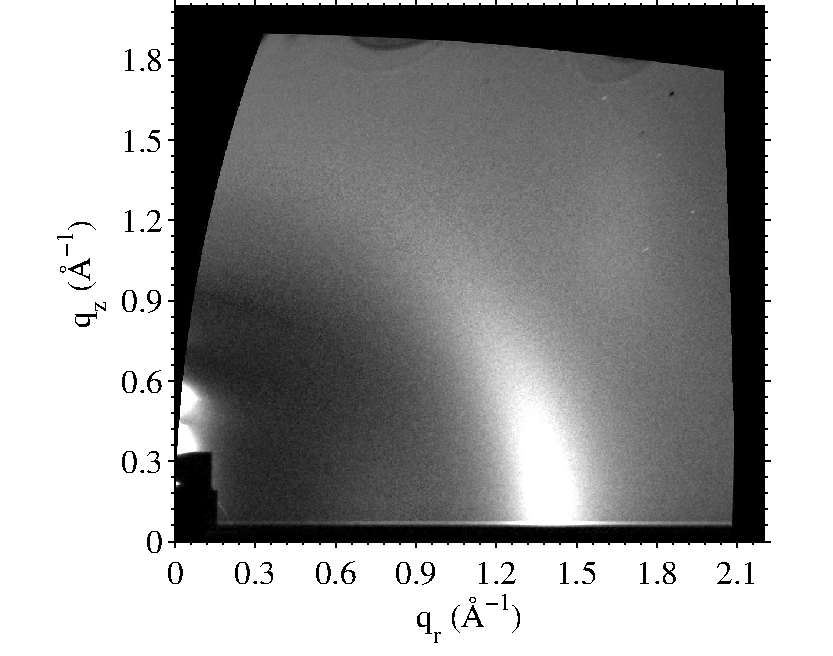
\includegraphics[width=0.45\textwidth]{figures/ripple/nGIWAXS/fluid_036}
  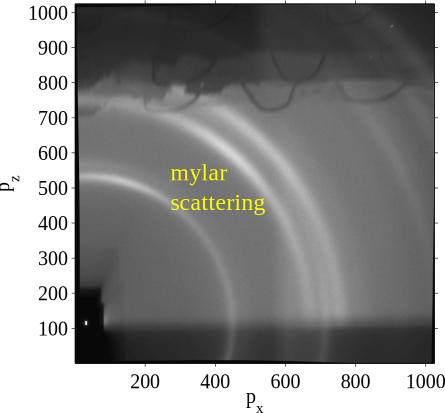
\includegraphics[width=0.45\textwidth]{figures/ripple/nGIWAXS/fluid_039}
  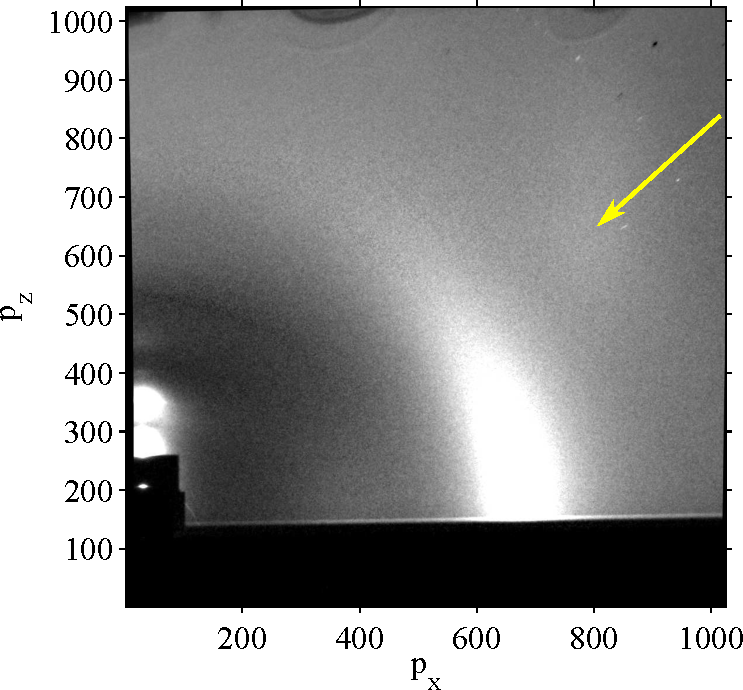
\includegraphics[width=0.45\textwidth]{figures/ripple/nGIWAXS/fluid_036_ccd}
  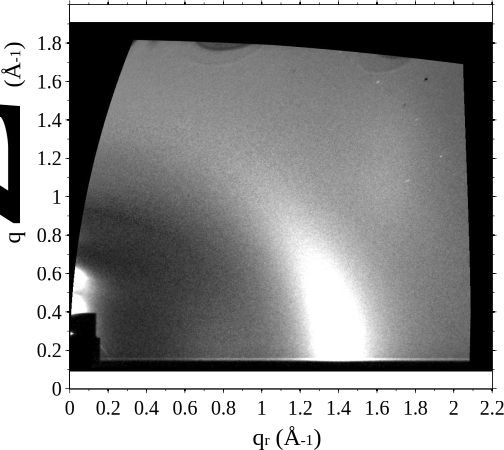
\includegraphics[width=0.45\textwidth]{figures/ripple/nGIWAXS/fluid_036_q}
  \caption[Data reduction of nGIWAXS data]
  {Data reduction of nGIWAXS data. (top) Fluid phase scattering at
  30 \textcelsius\ taken at $\omega$ = 0.5\textdegree\ (left) 
  and at -0.5\textdegree\ (right) with the low resolution setup at the 
  2011 run. The sample width $w_s$ = 2 mm.
  The fluid phase LAXS is also visible near the beam.  
  The darker region below the equator defined by 
  the beam vertical position $p_z$ was due to the substrate. The beam
  was visible through the semitransparent beam stop.
  Scattering at $p_z >$ 750 was the shadow cast by the electrical wires 
  and thermal shielding in the hydration chamber.
  (bottom) The background subtracted 
  image (left) and corresponding image in the sample $q$-space (right).
  Except for some minor left over scattering, background and mylar scattering was 
  removed very nicely. A weak scattering feature pointed to by an arrow
  is from a silicon wafer as we verified by collecting WAXS from a bare 
  wafer. Because the meridian was not exactly along the vertical
  pixels, the background subtracted image was rotated by $\sim$1\textdegree\
  in the clockwise direction before the $q$-space transformation. The data
  reduction was done using MATLAB.}
  \label{fig:waxs_data_reduction}
\end{figure}

\begin{figure}[htbp]
  \centering
  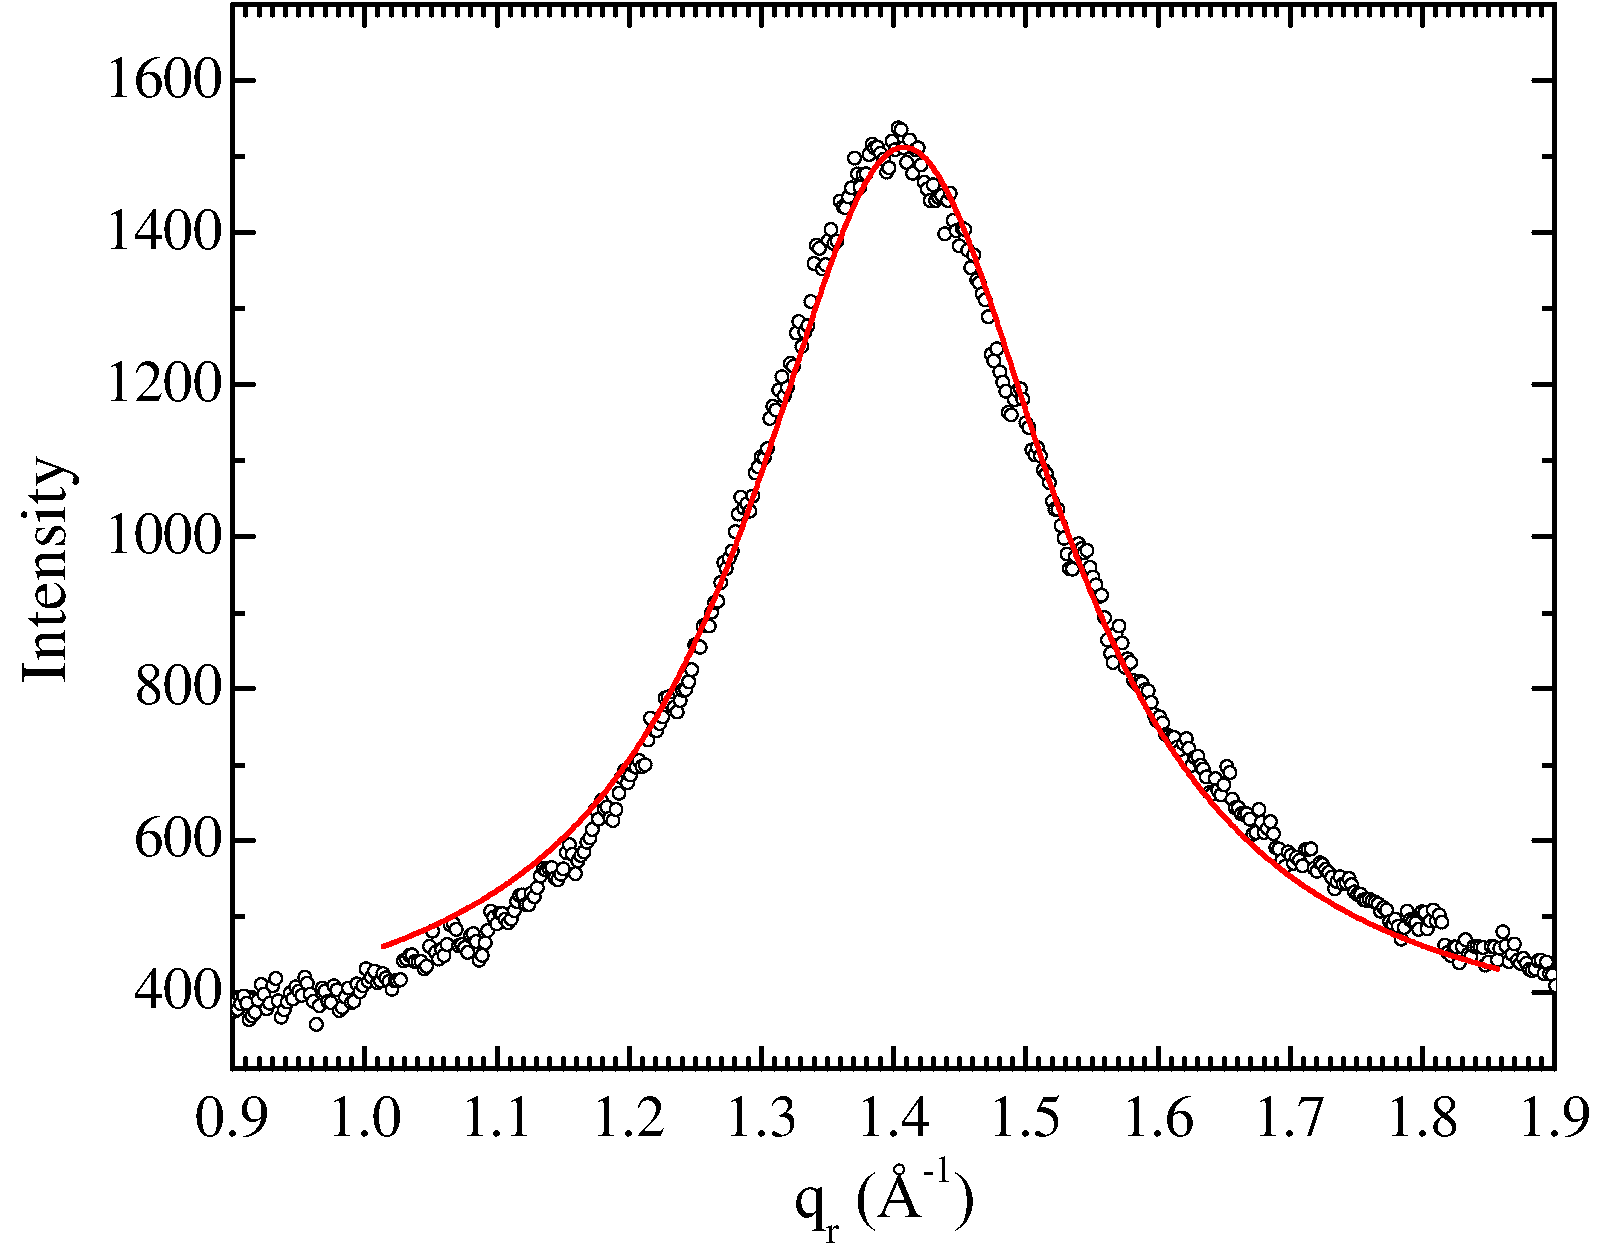
\includegraphics[width=0.7\textwidth]{figures/ripple/nGIWAXS/fluid_qr}
  \caption{Fluid phase WAXS plotted along $q_r$ at $q_z$ = 0.012 \AA$^{-1}$.
  The red solid line is a Lorentzian fit with its FWHM equal to 0.288 \AA$^{-1}$,
  centered at $q_r$ = 1.408. Extra intensity at larger $q_r$ was due to
  water scattering, which led to a slightly asymmetric profile.}
  \label{fig:fluid_qr}
\end{figure}

Figure~\ref{fig:gel_phase} shows nGIWAXS of the the DMPC L$_{\beta I}$ gel phase
that occurs at the highest hydration \cite{ref:Smith88,Tristram-Nagle02},
collected with the high resolution setup. Because exposure time was short,
the data did not have much intensity, but the (2,0) peak was clearly 
visible on the equator.
When the peak profile of the (2,0) peak in $q_r$ was fitted to a Lorentzian, 
we obtained an excellent fit with its FWHM $\Delta q_r = 0.014$ \AA$^{-1}$,
centered at $q_r$ = 1.479 \AA$^{-1}$.
This is the instrumental resolution as discussed in Sec.~\ref{sec:geometric_broadening}. 

\begin{figure}[htbp]
  \centering
  %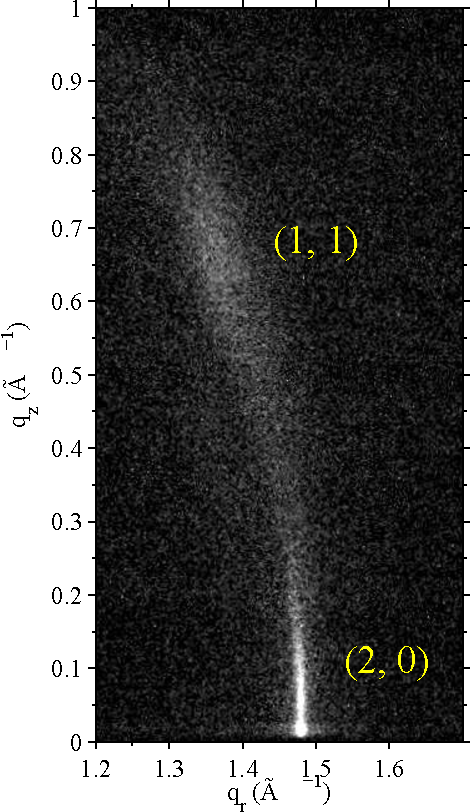
\includegraphics[trim=150 190 150 180,clip,width=0.45\textwidth]{figures/ripple/nGIWAXS/dmpc1_107}
  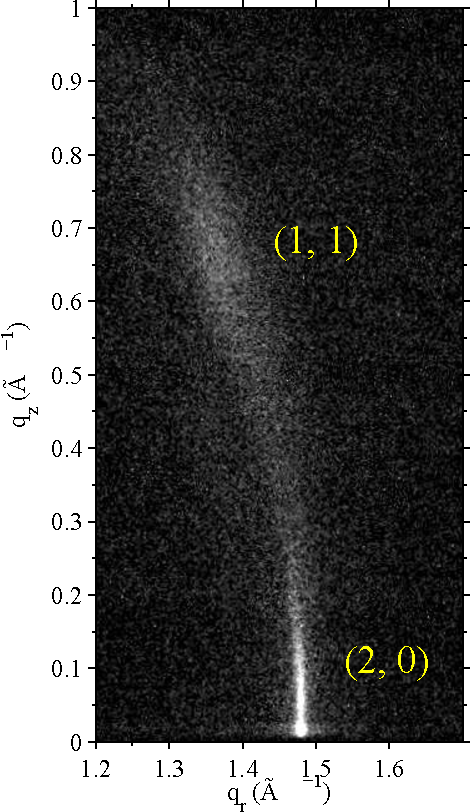
\includegraphics[width=0.4\textwidth]{figures/ripple/nGIWAXS/dmpc1_107}
  \qquad
  \includegraphics[trim=50 0 50 0,clip,width=0.45\textwidth]{figures/ripple/nGIWAXS/dmpc1_107_gel_phase_20_swath_8px}
  \caption[nGIWAXS of the DMPC gel phase]{(left) nGIWAXS image of the DMPC gel phase
  at 10 \textcelsius\ for $D$ = 57.7 \AA\ where the sample was in the 
  L$_{\beta I}$ phase. The Miller index for the (2, 0) and (1, 1) Bragg rods
  are shown in yellow. The (2, 0) peak was at
  $q_r=1.479$ \AA$^{-1}$, corresponding to $d_{20}=4.25$ \AA.
  (right) The (2, 0) peak plotted along horizontal pixels $p_x$. The solid red
  line is a Lorentzian fit to the data, resulting in the FWHM of $\sim$8 pixels,
  corresponding to $\Delta q$ = 0.014 \AA$^{-1}$,
  which is an unresolved width of intrinsically infinitely sharp peak
  estimated in Sec.~\ref{sec:instrumental_resolution}.}
  \label{fig:gel_phase}  
\end{figure}

\subsection{Ripple phase}\label{sec:nGIWAXS_ripple_phase}
Figure~\ref{fig:nGIWAXS_enlarge} shows nGIWAXS from an oriented DMPC film
in the ripple phase for $D$ = 60.8 \AA, collected with the high resolution setup. 
We observed a stronger peak and a weaker one off the equator. 
The maximum intensity of the stronger peak was at 
$(q_r, q_z) \approx (1.478 \pm 0.002 \text{ \AA}^{-1}, 0.20 \pm 0.01 \text{ \AA}^{-1})$ as shown
in Fig.~\ref{fig:qrplots}. The weaker peak was observed closer to the equator, and
separation of this peak from the stronger one was visible between 
$q_z$ = 0.10 and 0.14 \AA$^{-1}$, indicating that the center of this peak was approximately
$(q_r, q_z) \approx (1.457 \pm 0.004 \text{ \AA}^{-1}, 0.12 \pm 0.02 \text{ \AA}^{-1})$. 
Because of absorption of X-rays due to the sample, 
intensity became attenuated as one approaches the equator.
Very close to the equator, there is Vineyard-Yoneda 
peak that is due to constructive interference with scattering from the substrate,
which we will not consider.
Absorption and Vineyard-Yoneda peak did not affect determination of the 
ripple peak positions
as the ripple peaks were located at sufficiently large $q_z$. 
The positions of the peaks were consistent with those observed in 
transmission wide angle scattering, which is discussed in the next section.

\begin{figure}[htbp]
  \centering
  \includegraphics[trim=100 170 100 170,clip,width=\textwidth]{figures/ripple/nGIWAXS/dmpc1_enlarge}
  \caption{High resolution nGIWAXS of the DMPC ripple phase for $D$ = 60.8 \AA.
  The angle of incidence $\omega$ was 0.2\textdegree. The stronger peak was at
  $(q_r, q_z) \approx$ (1.478 $\pm$ 0.002 \AA$^{-1}$, 0.20 $\pm$ 0.01 \AA$^{-1}$). 
  The weaker peak was at 
  $(q_r, q_z) \approx$ (1.457 $\pm$ 0.004 \AA$^{-1}$, 0.12 $\pm$ 0.02 \AA$^{-1}$). The scattered
  intensity along the line slightly above $q_z$ = 0 \AA$^{-1}$ is the Vineyard-Yoneda
  peak \cite{ref:Vineyard82,ref:Miller08}.}
  \label{fig:nGIWAXS_enlarge}
\end{figure}

\begin{figure}[htbp]
  \centering
  \includegraphics[width=0.8\textwidth]{figures/ripple/nGIWAXS/qrplots}
  \caption{$q_r$ swaths of the ripple WAXS, each averaged over 0.02 \AA$^{-1}$
  in $q_z$. Each curve is shifted by 100 vertically. 
  The central $q_z$ values of swaths are shown in the figure legend.}
  \label{fig:qrplots}
\end{figure}

We also investigated dependence of the ripple WAXS on the interbilayer
$D$-spacing. Figure~\ref{fig:nGIWAXS} compares nGIWAXS at two different $D$-spacing,
showing that chain scattering did not depend on the $D$-spacing in this range. 
Figure~\ref{fig:nGIWAXS}(left) also shows a weak feature that looks like an 
arc coming from the chain peak. This feature extended
from $\phi$ = 0\textdegree\ to at least 70\textdegree, and
is likely to be scattering due to mosaic spread.

\begin{figure}[htbp]
  \centering
  \includegraphics[width=0.49\textwidth]{figures/ripple/nGIWAXS/dmpc1_046}
  \includegraphics[width=0.49\textwidth]{figures/ripple/nGIWAXS/046_vs_052}
  \caption{nGIWAXS of the DMPC ripple phase for $D$ = 59.2 \AA\ (left)
  and difference between $D$ = 59.2 \AA\ and 60.8 \AA\ (right). 
  The difference shows no obvious feature, indicating that the ripple WAXS
  patterns at the two D-spacing were identical within an error.
  The angle of incidence $\omega$ was 0.2\textdegree. The data were taken
  with the high resolution setup.}
  \label{fig:nGIWAXS}
\end{figure}

We estimated the width of the stronger peak by fitting 
the intensity profile in $q_r$ to double Lorentzian as shown in 
Fig.~\ref{fig:strong_peak}. The fit resulted in the FWHM $\Delta q_r$
= 0.025 \AA$^{-1}$ centered at 1.478 \AA$^{-1}$ and 
$\Delta q_r$ = 0.140 \AA$^{-1}$ centered at 1.464 \AA$^{-1}$.
A fit with a single Lorentzian was not very good, and 
a broader Lorentzian was necessary to produce a reasonable fit. 
We also fitted the peak profile in $q_r$ at $q_z$ = 0.12 \AA$^{-1}$,
where two distinct peaks were observed (Fig.\ref{fig:weak_peak}).
The two sharp peaks fitted with Lorentzian yielded the FWHM of about 
0.025 \AA$^{-1}$, consistent with the FWHM obtained for the stronger 
peak. The widths and positions of the observed peaks are summarized
in Table~\ref{tab:nGIWAXS_summary}.

As Fig.~\ref{fig:weak_peak}
shows, the double Lorentzian fit was only successful within a limited range
in $q_r$. This could be due to an underlining broad peak like the one
shown in Fig.~\ref{fig:strong_peak}. To investigate this possibility,
we fitted the same peak profile to triple Lorentzian with fixed widths.
Two of the Lorentzian had fixed widths of 0.025 \AA$^{-1}$ representing 
the sharp peaks and the last one had a fixed width of 0.14 \AA$^{-1}$
representing the broad peak. Figure~\ref{fig:weak_peak} shows an excellent
fit obtained over a large range in $q_r$, suggesting that the estimated
peak widths are not unreasonable.
Curiously, the center of the stronger peak was different at the two 
different $q_z$: ($q_r$, $q_z$) = (1.485 \AA$^{-1}$, 0.12 \AA$^{-1}$)
and (1.478 \AA$^{-1}$, 0.2 \AA$^{-1}$), while the total $q$ was about
the same, $\sim$1.49 \AA$^{-1}$.

\begin{figure}[htbp]
  \centering
  \includegraphics[width=0.7\textwidth]{figures/ripple/nGIWAXS/strong_peak_Lorentz}
  \caption[Peak profile in $q_r$ at $q_z$ = 0.2 \AA$^{-1}$ 
  fitted to double Lorentzian functions]{Peak profile in $q_r$ at $q_z$ = 0.2 \AA$^{-1}$ 
  fitted to double Lorentzian functions. The FWHM and center obtained 
  were 0.025 \AA$^{-1}$ and 1.478 \AA$^{-1}$ (green) and 0.140 \AA$^{-1}$ 
  and 1.464 \AA$^{-1}$(red), respectively. The solid blue line is a sum
  of the two Lorentzian fits.}
  \label{fig:strong_peak}
\end{figure}

\begin{figure}[htbp]
  \centering
  \includegraphics[width=0.45\textwidth]{figures/ripple/nGIWAXS/weak_peak_Lorentz}
  \includegraphics[width=0.45\textwidth]{figures/ripple/nGIWAXS/weak_peak_tripleLorentz}
  \caption[Peak profile in $q_r$ at $q_z$ = 0.12 \AA$^{-1}$ fitted to
  double Lorentzian (left) and double pseudo Voigtian functions (right)]
  {(left) Peak profile in $q_r$ at $q_z$ = 0.12 \AA$^{-1}$ fitted to
  double Lorentzian functions. 
  The FWHM and center obtained were 0.025 \AA$^{-1}$ and 1.457 \AA$^{-1}$ (red) 
  and 0.026 \AA$^{-1}$ and 1.484 \AA$^{-1}$ (green), respectively.
  The fit was limited within a range in which fits were reasonable.
  (right) The same peak profile fitted to triple Lorentzian. The FWHM was
  constrained to 0.025 \AA$^{-1}$ (blue), 0.025 \AA$^{-1}$ (green), and 0.14 \AA$^{-1}$ (red).
  The center was found to be 1.485 \AA$^{-1}$ (blue), 1.458 \AA$^{-1}$ (green), 
  and 1.458 \AA$^{-1}$ (red).}
  \label{fig:weak_peak}
\end{figure}

\begin{table}[htbp]
  \centering
  \begin{tabular}{ccccccc}
    \hline
    peaks & $q$ & $q_r$ & $q_z$ & $\Delta q_r$ & $\Delta q_z$ & $\hat{\theta}$ \\
     & (\AA$^{-1}$) & (\AA$^{-1}$) & (\AA$^{-1}$) & (\AA$^{-1}$) & (\AA$^{-1}$) & \\
    \hline
    stronger        & 1.491 $\pm$ 0.003 & 1.478 $\pm$ 0.002 & 0.20 $\pm$ 0.01 & 0.025 & 0.4 & 7.7\textdegree \\
    weaker          & 1.462 $\pm$ 0.006 & 1.457 $\pm$ 0.004 & 0.12 $\pm$ 0.02 & 0.025 & & 4.7\textdegree \\
    broader         & 1.463--1.478 & 1.458--1.464 & 0.12--0.20 & 0.140 & \\
    gel (2, 0)      & 1.479 & 1.479 & 0 & 0.014 & 0.4 & 0\textdegree \\
    gel ($\pm$1, 1) & 1.536 & \\
    fluid           & 1.41  &       &      & 0.288 & \\
    \hline
  \end{tabular}
  \caption[Summary of peak properties]
  {Summary of measured peak properties. 
  The $q$ value of gel ($\pm$1, 1) is taken from \cite{Tristram-Nagle02}.  
  The values of $\Delta q_z$ are 
  from Sec.~\ref{sec:tWAXS_results}. $\hat{\theta} = \arctan(q_z/q_r)$.
  $R = I_{strong}/I_{weak} \approx$ 1.5-1.85.}
  \label{tab:nGIWAXS_summary}
\end{table}

%\begin{figure}[htbp]
%  \centering
%  \includegraphics[width=0.6\textwidth]{figures/ripple/nGIWAXS/weak_peak_pseudoVoigt}
%  \caption[]
%  {The peak profile fitted to double pseudo Voigtian functions.
%  The FWHM and center obtained were 0.107 \AA$^{-1}$ and 1.458 \AA$^{-1}$ (red) 
%  and 0.077 \AA$^{-1}$ and 1.484 \AA$^{-1}$ (green), respectively.
%  The Gaussian FWHM in the pseudo Voigt was fixed to 0.014 \AA$^{-1}$.}
%  \label{fig:pseudoVoigt}
%\end{figure}


%{\color{blue}While it is possible to argue that 
%the long tail of the ripple peak is due to fluid like chain correlation
%in the minor arm, subtraction of the fluid phase WAXS from the ripple phase
%WAXS results in a underlining ripple peak that is asymmetric (Fig.~\ref{fig:ripple-fluid}).
%Therefore, chain packing in the minor arm is likely to be different from that 
%in the fluid phase.}
%blah
%\textcolor{red}{This stuff is already about hypothesis evaluation. It might
%be more appropriate to do this in the Discussion section.}



%\begin{figure}[htbp]
%  \centering
%  \includegraphics[width=0.45\textwidth]{figures/ripple/nGIWAXS/qr_fluid&ripple0}
%  \includegraphics[width=0.45\textwidth]{figures/ripple/nGIWAXS/qr_fluid&ripple1}
%  \includegraphics[width=0.45\textwidth]{figures/ripple/nGIWAXS/qr_fluid&ripple2}
%  \includegraphics[width=0.45\textwidth]{figures/ripple/nGIWAXS/qr_fluid&ripple3}
%  \includegraphics[width=0.45\textwidth]{figures/ripple/nGIWAXS/qr_fluid&ripple4}
%  \includegraphics[width=0.45\textwidth]{figures/ripple/nGIWAXS/qr_fluid&ripple5}
%  \caption{$q_r$ swaths comparing intensity of the fluid WAXS and ripple WAXS.
%  The fluid phase data were scaled so that its WAXS lies below the ripple WAXS.}
%  \label{fig:fluid&ripple}
%\end{figure}

%\begin{figure}[htbp]
%  \centering
%  \includegraphics[width=0.45\textwidth]{figures/ripple/nGIWAXS/qr_ripple-fluid}
%  \caption{Subtraction of the fluid phase WAXS from the ripple phase
%  WAXS. The subtraction results in asymmetric ripple peak.}
%  \label{fig:ripple-fluid}
%\end{figure}



%%%%%%%%%%%%%%%%%%%%%%%%%%%%%%%%%%%%%%%%%%%%%%%%%%%%%%%%%%%%%%%%%%%%%%%%%%%%%%%
\newpage
\section{tWAXS: results}\label{sec:tWAXS_results}
Figure~\ref{fig:twaxs_gel}(left) shows background subtracted transmission wide
angle X-ray scattering (tWAXS) of the DMPC gel \LbetaI\ phase obtained at 
$\omega$ = 45\textdegree.
The background scattering image was collected by replacing 
the sample with a bare Si wafer. Imperfect subtraction of mylar scattering 
can be seen in the background subtracted image. 
This was most likely due to slight displacement of mylar windows
when the sample was replaced with a bare wafer. 
Three main reflections whose Miller indices 
are (2,0), (1,1), and (1,-1) were observed along with the (1,$\pm$1) satellite 
peaks.
Because the data were taken at $\omega=45$\textdegree, the WAXS pattern 
appeared on the CCD detector very differently from the respective pattern
in the sample $q$-space. 
Therefore, the CCD to $q$-space transformation shown in 
Fig.~\ref{fig:twaxs_gel}(right) was important in analyzing the tWAXS data. 

Figure~\ref{fig:twaxs_ripple} shows the tWAXS pattern of the ripple phase 
after the CCD to q transformation. The stronger
peak observed in nGIWAXS was also observed at approximately the same location.
Because of a lower instrumental resolution than in the nGIWAXS experiment,
the weaker peak was not as well separated. Figure~\ref{fig:twaxs_weak_qr} shows
a hint of the weak peak at $q_z=0.12$ \AA$^{-1}$. This
data set taken in the 2011 run motivated me to try an experiment
with a higher instrumental resolution, which led to the nGIWAXS experiment
in the 2013 run. 

The length $L$ of scattering entities in the $z$ direction can be estimated by 
measuring the full length $\Delta q_z$ of the (2,0) Bragg rod in $q_z$ in
the $L_{\beta I}$ phase \cite{ref:Tristram93},
the relation between them being $\Delta q_z = 4\pi/L$.
Figure~\ref{fig:twaxs_gel_qz} shows intensity of observed Bragg rods along $q_z$ averaged in $q_r$
for the gel and ripple phases. The full length $\Delta q_z$ for the (2,0) gel
phase peak was measured to be $\sim$0.4 \AA$^{-1}$, corresponding to 
$L \approx 31$ \AA. This value of $L$ indicates that chains in the upper and
lower monolayers scatter coherently, which has been shown to be the case
for DPPC previously \cite{ref:Tristram93}.
Figure~\ref{fig:twaxs_gel_qz}(right) compares $\Delta q_z$ in the ripple and gel phases,
showing that $\Delta q_z$ was almost the same in both phases. Therefore, 
chains in the major arm are also coupled between the monolayers. 
We note that mosaic spread of the sample would make the apparent $\Delta q_z$ 
larger, so that $L \approx 31$ \AA\ might be the lower bound on the true $L$. 

Finally, Fig.~\ref{fig:twaxs_qzplot} plots $q_z$ swath along the weaker 
Bragg rod and along the entire ripple WAXS pattern. 
We found no obvious intensity maxima
near the equator, asserting that the weaker peak was also
off the equator as discussed in Sec.~\ref{sec:nGIWAXS_results}.
We also found no sign of a third peak.

\begin{figure}[htbp]
  \centering
  \includegraphics[width=0.44\textwidth]{figures/ripple/tWAXS/twaxs_gel_ccd}
  \includegraphics[width=0.54\textwidth]{figures/ripple/tWAXS/twaxs_gel_q}
  \caption[Transmission WAXS of the DMPC gel phase]
  {Transmission WAXS of the DMPC gel $L_{\beta I}$ phase observed on
  the CCD detector (left) and its corresponding pattern in the sample $q$-space
  (right). Bragg rods were indexed as (2,0), (1,1) and (1,-1). The satellite 
  peaks of (1,$\pm$1) reflections were also labeled. The black region in
  the right image corresponds to $q$-space that was not probed. The edges
  of the sample $q$-space image were distorted due to the nonlinear relation
  between the detector pixels and the sample $q$-space as discussed in 
  Sec.~\ref{sec:nGIWAXS_results}. A ring of intensity
  at $q \approx$ 0.9 \AA$^{-1}$ is due to imperfect subtraction of the mylar
  scattering. Residual mylar scattering is also visible near the (2,0) Bragg 
  rod.}
  \label{fig:twaxs_gel}
\end{figure}

\begin{figure}[htbp]
  \centering
  \includegraphics[trim=20 0 10 0,clip,width=0.5\textwidth]{figures/ripple/tWAXS/twaxs_ripple}
  \caption[tWAXS image of the DMPC ripple phase]{tWAXS image of the DMPC
  ripple phase at 18 \textcelsius\ and $D$ = 60.3 \AA.}
  \label{fig:twaxs_ripple}
\end{figure}

\begin{figure}[htbp]
  \centering
  \includegraphics[width=0.5\textwidth]{figures/ripple/tWAXS/twaxs_weak_qr}
  \caption{$q_r$ swath of the ripple tWAXS at $q_z$ = 0.12 \AA$^{-1}$. 
  Asymmetric shape of the profile is due to
  two Bragg rods centered at different $q_r$ values as discussed in
  Sec.~\ref{sec:nGIWAXS_results}.}
  \label{fig:twaxs_weak_qr}
\end{figure}

\begin{figure}[htbp]
  \centering
  \includegraphics[width=0.45\textwidth]{figures/ripple/tWAXS/twaxs_gel_qz}
  \includegraphics[width=0.45\textwidth]{figures/ripple/tWAXS/twaxs_strong_qz}
  \caption[]{(left) $q_z$ swath of the gel (2,0) Bragg rod. The solid line is
  a Gaussian fit with the FWHM of 0.23 \AA$^{-1}$. 
  (right) $q_z$ swath of the ripple peak along the stronger peak 
  (red solid squares) and the gel (2,0) peak scaled and shifted to guide 
   visual comparison (open black circles).}
  \label{fig:twaxs_gel_qz}
\end{figure}

\begin{figure}[htbp]
  \centering
  \includegraphics[width=0.45\textwidth]{figures/ripple/tWAXS/twaxs_weak_qz}
  \includegraphics[width=0.45\textwidth]{figures/ripple/tWAXS/twaxs_both_qz}
  \caption{$q_z$ swath along the weaker peak (left) and 
  along the entire ripple WAXS pattern (right).}
  \label{fig:twaxs_qzplot}
\end{figure}  

%\begin{figure}[htbp]
%  \centering
%  \includegraphics[width=0.3\textwidth]{figures/ripple/tWAXS/twaxs_qrplot2}
%  \includegraphics[width=0.3\textwidth]{figures/ripple/tWAXS/twaxs_qrplot3}
%  \includegraphics[width=0.3\textwidth]{figures/ripple/tWAXS/twaxs_qrplot4}
%  \includegraphics[width=0.3\textwidth]{figures/ripple/tWAXS/twaxs_qrplot5}
%  \includegraphics[width=0.3\textwidth]{figures/ripple/tWAXS/twaxs_qrplot6}
%  \includegraphics[width=0.3\textwidth]{figures/ripple/tWAXS/twaxs_qrplot7}
%  \includegraphics[width=0.3\textwidth]{figures/ripple/tWAXS/twaxs_qrplot8}
%  \includegraphics[width=0.3\textwidth]{figures/ripple/tWAXS/twaxs_qrplot9}
%  \includegraphics[width=0.3\textwidth]{figures/ripple/tWAXS/twaxs_qrplot9}
%  \includegraphics[width=0.3\textwidth]{figures/ripple/tWAXS/twaxs_qrplot10}
%  \includegraphics[width=0.3\textwidth]{figures/ripple/tWAXS/twaxs_qrplot11}
%  \includegraphics[width=0.3\textwidth]{figures/ripple/tWAXS/twaxs_qrplot12}
%  \caption{$q_r$ swaths of the tWAXS image, each averaged over 0.02 \AA$^{-1}$. 
%  The center $q_z$ value of a swatch is shown in the figure legends.}
%  \label{fig:twaxs_qrplots}
%\end{figure}

%%%%%%%%%%%%%%%%%%%%%%%%%%%%%%%%%%%%%%%%%%%%%%%%%%%%%%%%%%%%%%%%%%%%%%%%%%%%%%
\newpage
\section{Thin Rod Model}
\subsection{Gel phase model}
The fully hydrated gel phase of DMPC consists of hydrocarbon chains that are 
basically straight and cooperatively tilted by an angle $\theta$ from the 
bilayer normal \cite{ref:Smith88,ref:Tristram93,ref:Sun94,Tristram-Nagle02}. 
This is called the $L_{{\beta}I}$ phase in which each chain is tilted toward 
a nearest neighbor chain. At lower hydration the chains tilt differently. 
We will also focus on the $L_{{\beta}F}$ phase in this section.  The chains 
will be modeled as thin rods.  The basic geometry of the $L_{{\beta}I}$ phase 
is shown in Fig. 2 from Sun et al. 1994.  That study emphasized that the chains 
are tilted in the same direction in both monolayers. It also allowed for 
translational offsets that we will set to zero for simplicity.  

The unit cell that is customarily employed is indicated in Fig. 1c.  
For the $L_{{\beta}I}$ phase the chain are tilted along the $b$ direction 
as shown in Fig. 1b and along the $a$ direction for the $L_{{\beta}F}$ phase.  
It may be noted that chain packing in a plane that is perpendicular to the 
chains (and therefore not parallel to the bilayer) is nearly hexagonal; if 
the packing were hexagonal and if the chains had zero tilt, then in Fig. 1c 
one would have $b=a/\sqrt{3}$, which becomes $b=a/cos{\theta}\sqrt{3}$ with tilt.  
The Laue conditions for allowed reflections are 
\begin{equation}\label{Laue1}
q_x=2{\pi}m/a 
\end{equation}
and
\begin{equation}\label{Laue2}
q_y=2{\pi}n/b 
\end{equation}
which establish the location of possible lines of scattering (Bragg rods). 
The modulation of the intensity along these rods is derived from the square 
of the unit cell form factor
\begin{equation}\label{S(q)}
F(\mathbf{q}) = \int_{0}^{a}dx\int_{0}^{b}dy\int_{-(L/2)cos{\theta}}^{(L/2)cos{\theta}}dz\rho(\bold{r})exp(i\bold{q}\cdot\bold{r})
\end{equation}
Our thin rods are modeled as delta functions
\begin{equation}\label{rods}
\rho(\bold{r})=\delta(x-{\alpha}z,y-{\beta}z)+\delta(x-a/2-{\alpha}z,y-b/2-{\beta}z)
\end{equation}
where for the general case that the chain tilt is oriented at angle $\phi$ 
relative to the $x$ axis 
\begin{equation}\label{alpha}
\alpha=tan{\theta}cos{\phi}
\end{equation}
and
\begin{equation}\label{beta}
\beta=tan{\theta}sin{\phi}.
\end{equation}
For the $L_{{\beta}I}$ phase, $\phi={\pi}/2$ and for the $L_{{\beta}F}$ phase, 
$\phi=0$ .  Continuing with the general $\phi$ case for awhile,
defining $\gamma = {\alpha}q_x+{\beta}q_y+q_z$ yields
\begin{equation}\label{S(q)}
F(\bold{q}) = \int_{-(L/2)cos{\theta}}^{(L/2)cos{\theta}}dz\rho(\bold{r})e^{(i{\gamma}z}(1+e^{q_xa/2+q_yb/2}).
\end{equation}
The phase factor $1+e^{q_xa/2+q_yb/2}$ vanishes unless the sum $m+n$ of the 
Laue indices $(mn)$ is even. Only the lowest orders $(\pm2,0)$ and $(\pm1,\pm1)$ 
have observable intensity.  For the simple thin rod model in Eq.~\ref{rods} 
\begin{equation}\label{int}
F(q_z) = (4/\gamma)sin({\gamma}Lcos{\theta}/2)
\end{equation}
so the intensity $|F(q_z)|^2$ is modulated along each Bragg rod and maximum 
intensity occurs when $\gamma=0$ which, upon reversing the convention for the 
sign of $q_z$, means that the wide angle peaks are centered at
\begin{equation}\label{centers}
q_z^{mn}={\alpha}q_x+{\beta}q_y=\alpha2\pi{m}/a+\beta2\pi{n}/b.
\end{equation}
For the $L_{{\beta}I}$ phase with ${\phi}={\pi}/2$, one has
\begin{equation}\label{20LbI}
0=q_{z{\beta}I}^{20}=q_{z{\beta}I}^{-20}
\end{equation}
\begin{equation}\label{11LbI}
(2\pi/b)tan{\theta}=q_{z{\beta}I}^{11}=q_{z{\beta}I}^{-11}=-q_{z{\beta}I}^{1-1}=-q_{z{\beta}I}^{-1-1}
\end{equation}
For the $L_{{\beta}F}$ phase with ${\phi}=0$
\begin{equation}\label{20LbF}
(4\pi/a)tan{\theta}=q_{z{\beta}F}^{20}=-q_{z{\beta}F}^{-20}
\end{equation}
and
\begin{equation}\label{11LbF}
(2\pi/a)tan{\theta}=q_{z{\beta}F}^{11}=q_{z{\beta}F}^{1-1}=-q_{z{\beta}F}^{-11}=-q_{z{\beta}F}^{-1-1}
\end{equation}
One can verify, using these equations and the Laue equations for $q_x$ and $q_y$ 
that the magnitudes $q^{{\pm}20}$ and $q^{{\pm}1{\pm}1}$ of the total scattering 
vectors are equal when the packing of the chains is hexagonal in the tilted chain 
plane.  

In $\bold{q}$-space the powder averaged gel phase pattern consists of circles 
in $q_x$ and $q_y$ centered on $q_x=0=q_y$ and with the values of $q_z$ given 
in Eqs.~\ref{20LbI}-\ref{11LbF}.  
The location of observed scattering in lab space $\bold{k}$ is obtained using 
the Ewald sphere, centered at $\bold{k}=0$ with radius $2\pi/\lambda$ and with 
the $\bold{q}=0$ center of the $\bold{q}$-space pattern located 
at $\bold{k}=(0,|\bold{k}|,0)$.  The $\bold{q}$-space pattern is tilted by the 
angle $\omega$ when the sample is tilted relative to the laboratory frame; for 
grazing incidence, the $q_z$ and $k_z$ axes are parallel and offset 
by $2\pi/\lambda$ in the $k_y$ beam direction.  The direction of scattering for 
the powder averaged gel phase is given by the laboratory $\bold{k}$ values 
where the $q$-space pattern intersects the Ewald sphere.  Each of the $(mn)$ 
rings generally intesects twice with opposite signs for $k_x$ corresponding to 
opposite sides of the meridian on the CCD.  The only rings that give obervable 
scattering in the gel phase are the $(\pm20)$ and the $(\pm1\pm1)$ rings.  
However, some of these six rings may coincide. For the $L_{{\beta}I}$ phase 
$(\pm20)$, $(\pm11)$ and $(\pm1-1)$ are pairwise identical, so there are three 
primary reflections on each side of the merician. For the $L_{{\beta}F}$ phase 
$(1\pm1)$ and $(-1\pm1)$ are pairwise identical, so there are four primary peaks 
on each side of the meridian.

\subsection{Ripple model}
A reasonable hypothesis is that the major arm of the ripple has similar 
internal structure to a gel phase, with the major   difference that the plane 
of the major arm is tilted relative to the substrate.  That suggests that the 
predicted ripple pattern might be the same as would be obtained by tilting the 
in-plane powder averaged gel phase.  However, this would be a fundamental error 
because the operations of tilting and in-plane powder averaging do not commute.  
It is necessary first to tilt the gel phase $\bold{q}$-space pattern and then to 
powder average it about the laboratory $k_z$ axis.  

Furthermore, the axis for tilting matters, so it is important to define all 
angles carefully.  We continue to define the chain tilt angle relative to the 
bilayer normal by $\theta$.  The tilt of the major arm will be defined by a 
rotation angle $\xi$ about an axis in the $(x,y)$ plane and the angle that 
this axis makes with the $x$ axis will be defined to be $\zeta$.  Starting 
from the $q$ values obtained for the various gel phases, the proper order of 
rotations is first to rotate the orientation of the lattice with respect to 
the lab frame; this involves the standard rotation of the $(x,y)$ plane about 
the $z$ axis by angle $\zeta$.  Then, the gel phase is rotated about the new 
in-plane $x$ axis. The rotated $q$ value will be denoted $\tilde{q}$ which 
has components
\begin{equation}\label{qtz}
\tilde{q}_{z}^{mn}=q_{z}^{mn}cos{\xi}+q_{x}^{mn}sin{\xi}sin{\zeta}-q_{y}^{mn}sin{\xi}cos{\zeta},
\end{equation}
\begin{equation}\label{qtx}
\tilde{q}_{x}^{mn}=q_{x}^{mn}cos{\zeta}+q_{y}^{mn}sin{\zeta},
\end{equation}
and
\begin{equation}\label{qty}
  \tilde{q}_{y}^{mn} = q_{y}^{mn}\cos\xi\cos\zeta -
                       q_{x}^{mn}\cos\xi\sin\zeta +
                       q_{z}^{mn}\sin\xi.
\end{equation}
As there are many domains in each x-ray exposure, the next step powder averages 
each $(mn)$ reflection by rotating about the $z$ axis from $0$ to $2\pi$.  
As for the gel phase, the ensuing $q$ space pattern consists of circles parallel 
to the $(x,y)$ plane with center at $(0,0,q_z^{mn})$.  As noted above for the 
gel phase, this pattern is tilted by $\omega$ when the substrate is tilted for 
our transmission experiments.  Intersections of these circles with the Ewald 
sphere determines the angle of scattering in the laboratory from which, by 
standard equations (Section 3.2.6?), the $\bold{q}_{mn}$ are determined.  

The most pertinent component is $\tilde{q}_z^{mn}$ as this primarily determines 
how far reflections are from the meridian.  As there are many variable angles, 
let us consider $\tilde{q}_z^{mn}$ for the most pertinent special cases.  It is 
appropriate here to consider only $\omega=0$ because experimental data with 
$\omega{\neq}0$ are easily converted to this standard orientation.  We will 
focus on four special cases.  First, consider the in-plane orientation ${\zeta}$ 
of the lattice to have either the longer $a$ axis parallel (${\zeta}=0$) or 
perpendicular (${\zeta}={\pi}/2$) to the ripple direction.  It may be noted 
that these two special directions allow uniform packing of the unit cells along 
the finite ripple direction, whereas the edges of the unit cells are ragged at 
the boundaries of the major arm for other values of ${\zeta}$.  Also, these two 
directions are symmetrical.  However, as the lipid molecules are chiral and as 
there is likely disorder at the boundaries of the major arm, one cannot 
eliminate general ${\zeta}$ angles {\it a priori}.  We will also focus on the 
special orientations of the tilt direction that correspond to the $L_{{\beta}I}$ 
gel phase ($\phi=\pi/2$), which we will henceforth call $P_{{\beta}I}^{\zeta}$ 
phases, and the $L_{{\beta}F}$ gel phase ($\phi=0$), to be called 
$P_{{\beta}F}^{\zeta}$ phases, recognizing, of course, that we are only modeling 
the major arm of the $P_{\beta}$ ripple phase.   It will also be convenient to 
simplify to hexagonal packing of the hydrocarbon chains as the orthorhombic 
symmetry breaking that makes $q_{total}^{20}{\neq}q_{total}^{11}$ is small; 
then, $b=a/(\sqrt{3}cos{\theta})$ for the $P_{{\beta}I}^{\zeta}$ phases and 
$b=acos{\theta}/\sqrt{3}$ for the $P_{{\beta}F}^{\zeta}$ phases.  These 
simplifications allow us to focus on the chain tilt angle $\theta$ and the 
tilt $\xi$ of the major side for four cases of $(\phi,\zeta)$ and the 
observable orders $({\pm}2,0)$ and (${\pm}1,{\pm}1)$.  The following table 
shows the values of $q_z^{mn}$, all divided by $2\pi/a$, for the various 
phases that include lattice orientations $\zeta$.  

Interestingly, tilting the gel phase to form putative ripple major arms breaks 
the degeneracy of some of the gel phase rings.  Most notably, all the 
degeneracies are broken in the $P_{{\beta}I}^{\zeta=\pi/2}$ special case and 
none are broken in $P_{{\beta}F}^{\zeta=\pi/2}$.  The magnitude of these 
symmmetry breaking are typically $4{\pi}sin{\xi}/a {\approx} 0.32 {\AA}^{-1}$  
for $\xi=12$ degrees, so Bragg rods overlap considerably, making clear 
identification of the sample phase challenging.
\vspace{0.5cm}

\begin{table}[htbp]
\centering
\begin{tabular}{ | l | c | c | c |}
  \hline                       
   & $(\pm2,0)$ & $(\pm1,1)$ & $(\pm1,-1)$ \\
  \hline
 $L_{{\beta}I}$ & 0 & $\sqrt{3}\sin\theta$ & $-\sqrt{3}\sin\theta$\\
  \hline  
  $P_{{\beta}I}^{\zeta=0}$ & 0 & $\sqrt{3}\sin(\theta-\xi)$ & $-\sqrt{3}sin(\theta-\xi)$ \\
 \hline
  $P_{{\beta}I}^{\zeta=\pi/2}$ & $\pm2sin\xi$ & $\sqrt{3}sin{\theta}cos{\xi}\pm sin{\xi}$ & $-\sqrt{3}sin{\theta}cos{\xi}\pm sin{\xi}$\\
 \hline
& $(\pm2,0)$ & $(1,\pm1)$ & $(-1,\pm1)$\\
  \hline
$L_{{\beta}F}$ & $\pm2tan\theta$ & $tan\theta$ & $-tan\theta$ \\
 \hline
  $P_{{\beta}F}^{\zeta=0}$ & $\pm2\tan{\theta}\cos\xi$ & $\tan{\theta}\cos{\xi}\mp\sqrt{3}\sin{\xi}/\cos\theta$ & $-(\tan{\theta}\cos{\xi}{\mp}\sqrt{3}\sin{\xi}/\cos\theta)$\\
  \hline
   $P_{{\beta}F}^{\zeta=\pi/2}$ & $\pm2(tan{\theta}$cos$\xi+$sin$\xi$) & $tan{\theta}cos{\xi}+sin{\xi}$ & $-(tan{\theta}cos{\xi}+sin{\xi})$\\
  \hline
\end{tabular}
\caption{}
\label{tab:special_cases}
\end{table}

\begin{figure}[htbp]
  \centering
  \includegraphics[width=\textwidth]{figures/ripple/thin_rod_model/unit_cell_combined}
  \caption[Thin rod model]{
  (left) Projection of the unit cell ($a$, $b$) on the laboratory ($x$, $y$) plane.  
  The unit cell is rotated by $\zeta$ compared to parallel $a$ and $x$ and the 
  directions of chain tilt is rotated by $\phi$ from the $a$ axis. 
  (right) Without loss of generality, the ripple direction is shown along 
  the $y$ axis and the major side is tilted by $\xi$.  Supposing that the chains 
  are tilted in the $y$ direction only, then the corresponding gel phase could 
  be any L$_{\beta\text{L}}$ phase constrained only by 
  $\phi$ + $\zeta$ = $\pi/2$, including the 
  special L$_{\beta\text{I}}$ phase with $\phi=\pi/2$ and $\zeta=0$ and the 
  special L$_{\beta\text{F}}$ phase with $\phi=0$ and $\zeta=\pi/2$.}
  \label{fig:thin_rod_model}
\end{figure}

Our measured nGIWAXS pattern from the ripple phase described in
Sec.~\ref{sec:nGIWAXS_ripple_phase} revealed two sharp peaks whose centers 
were well above the equator. The only $P_{\beta}$ phase among the special
cases considered so far (Table~\ref{tab:special_cases})
that is compatible with our nGIWAXS data is $P_{\beta F}^{\zeta=\pi/2}$.
In this phase, the $q_z$ value of the (2, 0) peak is twice larger than ($\pm$1, 1),
which is consistent with our estimated peak positions, $q_z$ = 0.2 $\pm$ 0.01 and
0.12 $\pm$ 0.2. Then, the stronger peak can be indexed as (2, 0) and
the weaker one as (1, $\pm$1). The total $q$ of  
$P_{\beta F}^{\zeta=\pi/2}$ is $4\pi/(a\cos\theta)$. Using $\xi$ = 12\textdegree\ 
from Table~\ref{tab:LAXS_summary}, we can solve a set of two equations
for $q^{20}$ and $q_z^{20}$ involving $a$ and $\theta$, whose solution is
$a$ = 8.95 \AA\ and $\theta$ = 19.7\textdegree. From this value of $\theta$
and the value of $\DHH$ = 41 \AA\ from Table~\ref{tab:LAXS_summary},
the chain length $L$ can be estimated using $L=\DHH/\cos\theta$, which gives
$L$ = 43.5 \AA\.
In Ref.~\cite{Tristram-Nagle02}, the bilayer thickness $\DHH$ of the 
DMPC \LbetaI\ phase was reported to be 40.2 \AA\ with $\theta$ = 
32\textdegree, which gives $L$ = 47.4 \AA\ and consequently 
$a$ = 8.50 \AA.
Compared to the \LbetaI\ phase, our estimated chain length $L$ in the 
$P_\beta$ phase is smaller by about 4 \AA. 
This difference is consistent with the total $q$ values
of the $P_{\beta F}^{\zeta=\pi/2}$ peaks smaller than those of the \LbetaI\ peaks
(Table~\ref{tab:nGIWAXS_summary}),
indicating that the chain-chain distance is larger in the 
$P_{\beta F}^{\zeta=\pi/2}$ phase, which in turn implies that chains
in the $P_{\beta F}^{\zeta=\pi/2}$ phase are more disordered. This is 
reasonable because chains in the kink region are expected to be disordered,
which could cause the chain packing in the major arm to be different
from the gel phase. This may also explain the observed peak widths 
shown in Table~\ref{tab:nGIWAXS_summary} being larger than the width of
the \LbetaI\ (2, 0) peak. 

While the positions of the observed peaks are consistent
with a prediction of our thin model, 
integrated intensity of those peaks is not. Our model shows
that the peak at smaller $q_z$ is a superposition of (1, 1) and (1, -1) peaks,
giving a multiplicity factor of 2 for that peak.
This means that integrated intensity of the weaker peak should be twice 
that of the stronger peak, which is opposite of our results.
We also considered a possibility that the stronger peak is a superposition 
of two closely occurring (1, $\pm$1) or ($\pm$1, 1) peaks and 
the weaker one is indexed as (2, 0). 

\begin{table}[htbp]
  \centering
  \begin{tabular}{cccc}
    \hline
     & $a$ & $\theta$ & $L$ \\
     & (\AA) & & (\AA) \\
    \hline
    \LbetaI & 8.50 & 32\textdegree & 47.4 \\ 
    $P_{\beta F}^{\zeta=\pi/2}$ & 8.95 & 19.7\textdegree & 43.5 \\
    \hline
  \end{tabular}
  \caption{}
  \label{tab:waxs_structure}
\end{table}

%%%%%%%%%%%%%%%%%%%%%%%%%%%%%%%%%%%%%%%%%%%%%%%%%%%%%%%%%%%%%%%%%%%%%%%%%%%%%%%
\newpage
\section{Discussion}\label{sec:ripple_discussion}
\subsection{Major arm}
There has been a number of evidence to suggest that the major arm is like 
the gel phase. Figure~\ref{fig:gel_comparison} compares our electron density
profile in the major arm to the DMPC gel phase profile reported by 
Tristram-Nagle \textit{et al.} \cite{Tristram-Nagle02}. 
It shows that the density profile of the major arm is similar to that 
of the gel phase and the thickness is comparable between the two phases
although the ripple profile does not show distinction
between the phosphate and carbonyl-glycerol headgroups as in the gel phase.
Also, the terminal methyl trough appears to be wider in the ripple major arm,
which could be a sign that the terminal methyl is slightly more disordered
in the ripple phase than in the gel phase.
As discussed in
Sec.~\ref{sec:LAXS_edp}, however, small features in the ripple profile were not
reliable because they depended on which fitting results were used
to produce the electron density profile.
An important point we can make based on Fig.~\ref{fig:gel_comparison} 
is that chains must be tilted by some amount with respect to the local bilayer
normal. If we use the distance between the centers of the headgroups as the
bilayer thickenss, we have about 38 \AA\ for the gel phase and 40 \AA\
for the ripple phase. Because chains are tilted by 30\textdegree\ in the 
L$_{\beta I}$ phase, the chain tilt angle $\theta_t$ in the ripple major 
arm is roughly estimated to be 25\textdegree\ $\pm$ 1\textdegree. This constraint on $\theta_t$
and the measured $\alpha_M$ are important in understanding the nGIWAXS data.

\begin{figure}[htbp]
  \centering
  \includegraphics[width=0.45\textwidth]{figures/ripple/discussion/Tristram-Nagle_gel_DMPC}
  \includegraphics[width=0.45\textwidth]{figures/ripple/discussion/major_edp}
  \caption{Comparison of the electron density profiles of the DMPC gel phase (left)
  and the major arm in the ripple phase (right). The DMPC profile is taken from 
  Ref.~\cite{Tristram-Nagle02}. The ripple major arm profiles were calculated 
  using the phases predicted by Fit2, 5, and 7 (black, red, and green, respectively). 
  The ripple profiles are scaled to match 
  with the gel phase profile.}
  \label{fig:gel_comparison}
\end{figure}

While the electron density profile derived from the LAXS data indicates that 
chains are gel-like in the major arm, it does not show whether or not chains 
in different leaflets are coupled. To answer this question, we turned to
transmission WAXS where we were able to carefully measure the width of 
observed Bragg rods. Figure~\ref{fig:twaxs_gel_qz} shows that the widths of the Bragg
rods in the ripple and gel phases are approximately the same, indicating that
chains in different leaflets in the ripple major arm also scatter coherently.
This point can be contrasted with the chain packing in the major arm
observed in atomistic MD simulations by de Vries \textit{et al.} \cite{ref:deVries05}.
In their simulations, while chains were straightened out (all-trans) like in 
the case of the gel phase, their chain tilt angles $\hat{\theta}$ were modulated 
along the ripple direction. It was also
clearly seen in their simulations that chains in the different leaflets were 
decoupled and tilted in the opposite direction. Our tWAXS data are 
inconsistent with this picture and instead consistent with normal
gel phase packing where chains in different leaflets constitute long coherently
scattering entities.

\textcolor{red}{Regarding indexing the wide angle peaks}

The chain-chain correlation length can be estimated by using the Scherrer equation 
\cite{ref:Warren69},
\[
  B = \frac{0.94\lambda}{L\cos\theta},
\]
where $B$ is the observed FWHM of a Bragg peak, $\lambda$ is the wavelength,
$L$ is the length over which chains are positionally correlated, 
and $\theta$ is the Bragg angle. For the (2, 0) Bragg peak in
the gel L$_{\beta I}$ phase, we obtained the FWHM $\Delta q = 0.014$ \AA$^{-1}$ and
the position of the peak $q$ = 1.479 \AA$^{-1}$. For our X-ray wavelength
$\lambda$ = 1.175 \AA, the Scherrer equation yields $L$ = 426 \AA. 
Because the width of the (2,0) gel phase peak 
was not instrumentally resolved, the correlation length of chains was 
greater than 426 \AA.
The width of similar lipid, DPPC, was resolved and had a correlation 
length of 2900 \AA \cite{ref:Sun94}.

In contrast, the observed peaks in the ripple phase were instrumentally 
resolved (Fig.~\ref{fig:strong_peak}). 
The FWHM of the stronger peak was estimated to be 0.025 \AA$^{-1}$,
corresponding to the correlation length of $\sim$240 \AA,
indicating that the correlation length in the ripple phase is shorter 
than that in the gel phase.
This observation can be qualitatively understood by supposing that chains in the major
and minor arms are not correlated, so that gel phase like chains in the 
major arm are only correlated within the major arm, limiting the correlation
length along the ripple direction to be less than the length of the major 
arm, $\sim$100 \AA. Although
it is possible that chains are correlated over a much longer distance 
along the direction perpendicular to the ripple direction leading to
a sharp reflection along $q_y$,
what is observed in our in-plane powder sample is a convolution
of a broad width along $q_x$ and sharp one along $q_y$. Such convolution
would result in a broad Bragg rod as observed in our nGIWAXS data.
To quantitatively understand the observed peak widths would require to
model the finite size effect rigorously. This could lead to a prediction
for the peak shape that is not Gaussian assumed by the Scherrer equation 
\cite{ref:Warren69}, which we did not consider.

\subsection{Minor arm}
Some previous work have suggested that chains in the minor arm are disordered 
and fluid as in the L$_\alpha$ fluid phase.
Figure~\ref{fig:fluid_comparison} compares our electron density profiles
in the minor arm to the DMPC fluid phase profile reported by 
Kucerka \textit{et al.} \cite{Kucerka05_BPJ}.
Unlike in the case for the major arm, the density profile in the minor arm
does not resemble that of the fluid phase at all. This radically different
profile of the minor arm is not an artifact as we successfully obtained 
a typical bilayer profile for the major arm.
Inconsistency of the minor arm being like the fluid phase is also seen in our nGIWAXS data.
Figure~\ref{fig:fluid_vs_ripple} compares observed WAXS patterns of the ripple and 
fluid phase. The fluid phase pattern was centered at $q_r$ = 1.4 \AA$^{-1}$, where
there is no obvious feature in the WAXS pattern of the ripple phase. While one
could argue that the fluid phase pattern can be scaled down to match the tail
of the ripple Bragg peaks, thereby making the two consistent with each other, 
as previously argued in Ref.~\cite{ref:Cunningham98}, 
subtraction of the fluid phase pattern from the ripple pattern would result
in an asymmetric shape of the ripple Bragg peaks, which is not very reasonable.

Another type of chain packing, possibly with atypical bilayer profile, for the minor arm 
is the chain interdigitation proposed by de Vries \textit{et al.} \cite{ref:deVries05}.
Figure~\ref{fig:interdigitation_comparison} compares the electron density
profiles in the minor arm with that of the DHPC L$_\beta\text{I}$ interdigitated phase
reported by \cite{ref:Guler09}. Absence of the methyl trough can be seen in
both L$_\beta\text{I}$ phase and the ripple minor arm, but the widths of the
headgroups are much narrower in the DHPC L$_\beta\text{I}$ phase. The widths
of the ''headgroups'' in the minor arm profile are about 10 \AA, comparable
with those in the major arm profile. While Fig.~\ref{fig:interdigitation_comparison}
suggests that interdigitated chains are not completely inconsistent with 
out results in terms of an overall shape of the density profile, 
our nGIWAXS pattern clearly eliminates the packing proposed in 
Ref.~\cite{ref:deVries05}. Figure~\ref{fig:nGIWAXS_comparison} compares
the calculated wide angle pattern from their atomistic MD simulations
to our measured nGIWAXS pattern from the ripple phase. As noted in
Ref.~\cite{ref:deVries05}, interdigitated chains in the minor arm scatter
coherently, giving rise to a Bragg peak centered at $q_z \approx$ 0.4 \AA$^{-1}$.
This off-equator Bragg peak is due to chains being tilted by about 20\textdegree\
with respect to the stacking $z$ direction though they
are essentially parallel to the local bilayer normal.
We saw no sign of a Bragg peak at such large $q_z$ in our nGIWAXS
data, so our wide angle data do not support the structure proposed by
de Vries \textit{et al.} \cite{ref:deVries05}.

\begin{figure}[htbp]
  \centering
  \includegraphics[width=0.45\textwidth]{figures/ripple/discussion/Kucerka_fluid_DMPC}
  \includegraphics[width=0.45\textwidth]{figures/ripple/discussion/minor_edp}
  \caption{Comparison of the electron density profiles of the DMPC fluid phase (left)
  and the minor arm in the ripple phase (right). The DMPC profile is taken from 
  Ref.~\cite{Kucerka05_BPJ}. The ripple minor arm profiles were calculated 
  using the phases predicted by Fit2, 5, and 7 (black, red, and green, respectively). 
  The ripple profiles are scaled to match approximately
  with the fluid phase profile.}
  \label{fig:fluid_comparison}
\end{figure}

\begin{figure}[htbp]
  \centering
  \includegraphics[width=0.5\textwidth]{figures/ripple/nGIWAXS/fluid_vs_ripple}
  \caption{Comparison of the ripple (black) and fluid (red) phase WAXS at $q_z$ = 0.012 \AA$^{-1}$.
  The fluid phase data were taken with the low resolution setup and scaled 
  vertically to enable visual comparison.}
  \label{fig:fluid_vs_ripple}
\end{figure}

\begin{figure}[htbp]
  \centering
  \includegraphics[width=0.45\textwidth]{figures/ripple/discussion/Guler_interdigitated_DHPC}
  \includegraphics[width=0.45\textwidth]{figures/ripple/discussion/minor_edp}
  \caption{Comparison of the electron density profiles of the DHPC  
  L$_\beta\text{I}$ interdigitated phase (left)
  and the minor arm in the ripple phase (right). The DHPC profile is taken from 
  Ref.~\cite{ref:Guler09}. The ripple minor arm profiles were calculated 
  using the phases predicted by Fit2, 5, and 7 (black, red, and green, respectively). 
  The ripple profiles are scaled to match approximately
  with the L$_\beta\text{I}$ phase profile.}
  \label{fig:interdigitation_comparison}
\end{figure}

\begin{figure}[htbp]
  \centering
  \includegraphics[width=0.5\textwidth]{figures/ripple/discussion/deVries_waxs}
  \qquad
  \includegraphics[width=0.35\textwidth]{figures/ripple/discussion/ripple_waxs}
  \caption{Comparison of the wide angle (WAXS) pattern predicted by the 
  ripple phase structure proposed in Ref.~\cite{ref:deVries05} (left) and
  our measured WAXS (right). In the left, the interdigitated chains scatter 
  coherently, giving rise to a Bragg peak at $q_z \approx 0.4$ \AA$^{-1}$,
  while $q_z$ values of the observed peaks in our data were 0.12 \AA$^{-1}$
  and 0.2 \AA$^{-1}$.}
  \label{fig:nGIWAXS_comparison}
\end{figure}

%%%%%%%%%%%%%%%%%%%%%%%%%%%%%%%%%%%%%%%%%%%%%%%%%%%%%%%%%%%%%%%%%%%%%%%%%%%%%%%
\newpage
\section{Conclusion}\label{sec:ripple_conclusion}
The ripple phase has attracted many researchers since its discovery in 1967,
and extensive study on average structural properties such as 
the ripple wavelength, oblique angle, $D$-spacing, and electron density
profiles have been reported. From those experimental measurements, 
many theoretical models to explain the origin of the ripple phase have 
been considered. Yet, molecular packing in the asymmetric
ripple has only be elusive. 
Several work have suggested various molecular packing in this phase.
Based on the diffusion measurements that showed a fast component and
slow component, the idea of micro phase separation that the major arm
is gel like while the minor arm is fluid like was proposed. This idea
was supported by a later low angle X-ray study that showed the thickness of the major arm
is comparable to that of the gel phase while the thickness of the minor
arm is smaller. This work was then followed by a wide angle X-ray study on
unoriented samples, arguing that the micro phase separation is consistent 
with the wide angle data.
Another proposed molecular packing was based on the electron density profile
derived from X-ray form factors. Given that the model parameter that represents
the chain tilt was constant throughout the ripple bilayer, it was argued 
that chains were gel like in both major and minor arms with the same 
chain tilt angle with respect to the stacking $z$ direction.
More recently, a MD simulation proposed interdigitated chains in the minor 
arm while chains are gel like in the major arm but with decoupled leaflets.

Previous predictions and suggestions for molecular packing in the asymmetric
ripple so far have not been directly tested 
because of lack of a high quality electron
density profile and quantitative wide angle 
scattering data from an oriented sample.
Therefore, we sought to fill the gap
with synchrotron X-ray techniques. Our strength were three fold: 1) brilliant
synchrotron beam that allowed use of Si monochromater with a very small
energy dispersion, 2) stacks of $\sim$2000 bilayers oriented on the substrate
that scattered strongly and anisotropically, and 3) hydration chamber that 
allowed us to control the hydration of the sample with minimum background scattering.
While we could not calculate the electron density profile with high precision unambiguously
or solve the chain packing in the minor arm based on the measured wide angle scattering data, 
we were able to test the aforementioned proposed molecular packing.
Our new data sets should also facilitate testing variations of those proposed 
structure as well as new structures that will come forth in a future.
For example, Monte Carlo simulations based on a model free energy can be tuned
to obtain a good fit to our measured wide angle data.
One could also consider some exotic packing such as swirling pattern observed
in Ref.~\cite{ref:Watkins11}. Predicting the scattering
intensity pattern from these structures might lead to a different way
to analyze our LAXS and nGIWAXS data and possibly more improved study of the 
ripple phase. 

Future possible experiments
include a high resolution transmission experiment, where both geometric 
broadening and energy dispersion are minimized. The expected resolution 
is the width of the X-ray beam, which is about 3 pixels. This experiment 
doubles the best resolution achieved in this work. 
Another slightly different high resolution experiment is to use silicon 
crystal analyzer downstream of the sample, which completely remove geometric
broadening. The downside of this type of high resolution experiment is that
only one point in q-space is probed at any given exposure, so getting a full
2D map of wide angle scattering is time consuming.  

Also highly speculative, but the ripple phase might be an interesting phase
to study curvature sensing peptides. The description of curvature in the
ripple phase has been around for a while. Those curvature sensing peptides
may accumulate at the kink regions. Then, the electron density profile
can be calculated with the analysis detailed in this work. It would 
be very interesting if peptide-lipid interactions also significantly 
modify the wide angle pattern. With a known perturbation property of 
a peptide on lipids, it could shed light on the structure of the minor arm.
For example, if indeed chains are fluid like in the minor, some peptides
might have tendency to accumulate in the minor arm because of ease of 
insertion compared to the gel-like major arm.
Then, the ripple phase might be used to study biologically relevant problems.
